\documentclass[11pt,a4paper]{article}

\usepackage[margin=2.3cm]{geometry}
\usepackage[T1]{fontenc}
\usepackage[utf8]{inputenc}
\usepackage{lmodern}
\usepackage{amsmath,amssymb,amsthm}
\usepackage{booktabs,longtable,array}
\usepackage{graphicx}
\usepackage{xcolor}
\usepackage{tikz}
\usetikzlibrary{positioning,arrows.meta}
\usepackage[numbers,sort&compress]{natbib}
\usepackage{url}
% allow line breaks in file paths after these characters
\renewcommand{\UrlBreaks}{\do\/\do\_\do\.\do\-}
\usepackage[hidelinks]{hyperref}
\usepackage{caption}

% Figures are read from the repository (compilation inside report/) or, in the Overleaf archive,
% from figures/ (see package.py).
\graphicspath{{../experiments/}{../analysis/}{figures/}}

\newcommand{\todo}[1]{\textcolor{red}{[#1]}}
\newcommand{\obs}{\textsc{[Observed]}}
\newcommand{\hyp}{\textsc{[Hypothesized]}}
\newcommand{\ver}{\textsc{[Verified]}}
\newcommand{\openlbl}{\textsc{[OPEN]}}
\newcommand{\status}[1]{\hfill\textit{Status: #1}}
\newcommand{\tp}{^{\top}}
\newcommand{\Ex}{\mathbb{E}}
\newtheorem{proposition}{Proposition}

\newcommand{\LinNomNEES}{2.04 [1.99, 2.10]}
\newcommand{\LinNomNIS}{1.01 [0.998, 1.02]}
\newcommand{\LinScaleRMSEa}{2.70417}
\newcommand{\LinScaleRMSEb}{2.70417}
\newcommand{\LinScaleNEESa}{783.42}
\newcommand{\LinScaleNEESb}{0.78342}
\newcommand{\LinChiNEESinside}{94.5}
\newcommand{\LinChiNISinside}{97.0}
\newcommand{\LinChiSteps}{200}
\newcommand{\FFAdaptQdiv}{1}
\newcommand{\FFAdaptNomNEES}{4.36 [4.17, 4.56]}
\newcommand{\FFPairedSupported}{59}
\newcommand{\FFPairedTotal}{72}
\newcommand{\FFRuntimeEKF}{18.5}
\newcommand{\FFRuntimeIEKF}{125}
\newcommand{\FFRuntimeUKF}{35.3}
\newcommand{\FFRuntimeAdaptEKF}{31.7}
\newcommand{\AttRefSensorEarly}{24.5}
\newcommand{\AttRefSensorLate}{2.83}
\newcommand{\AttRefBodyZeroLate}{2.82}
\newcommand{\SFNotSupported}{3}
\newcommand{\SFTotal}{60}
\newcommand{\SFNISmaxchange}{0.730}
\newcommand{\SFNEESminchange}{6.53}
\newcommand{\SFNEESmaxchange}{2137}
\newcommand{\MisNISmaxchange}{0.124}
\newcommand{\DiagLinFiveTotal}{0.926 [0.837, 1.02]}
\newcommand{\DiagLinFiveFeedback}{0.475 [0.418, 0.538]}
\newcommand{\DiagLinFiveOwnData}{0.0516 [-0.0199, 0.122]}
\newcommand{\DiagLinFiveFluct}{0.399 [0.345, 0.453]}
\newcommand{\DiagLinFiveClosedStats}{0.794 [0.694, 0.898]}
\newcommand{\TVPairedTotal}{216}
\newcommand{\TVPairedWorse}{203}
\newcommand{\TVPairedBetter}{0}
\newcommand{\NRWinBurst}{10}
\newcommand{\NRWinPooled}{20}
\newcommand{\GTwoGRU}{45}
\newcommand{\GTwoMLP}{57}
\newcommand{\BoundGRU}{12.68}
\newcommand{\BoundMLP}{8.805}
\newcommand{\TrainMaxFactor}{25.0}
\newcommand{\TrainMaxFactorPct}{2.36}
\newcommand{\GRUalphaAtTwentyFive}{10.2}
\newcommand{\GRUalphaTrainTwentyFive}{10.3}


\title{Classical, Adaptive and Learning-Assisted Kalman Filtering under Measurement-Noise
Variation, Inertial-Model Mismatch and GNSS-Denied Conditions}
\author{}
\date{}

\begin{document}
\maketitle

\begin{abstract}
This report investigates the behavior of classical, adaptive, and learning-assisted Kalman
filtering approaches under measurement-noise variation, inertial-model mismatch, and GNSS-denied
conditions. Using controlled synthetic experiments and real-world inertial data characterization,
we examine estimation accuracy, statistical consistency, covariance adaptation, and the
limitations of commonly used filtering assumptions. A recurrent neural covariance estimator
demonstrates improvements under selected transient-noise conditions, while negative controls and
held-out evaluations reveal limitations in calibration and generalization. These findings
provide an evidence-based foundation for determining which filtering components may benefit from
learning and which require explicit physical modeling or calibration.
\end{abstract}

%==================================================================================================
\section{Scope and research questions}\label{sec:scope}
%==================================================================================================

The advisor asked four questions: (Q1) what assumptions the members of the Kalman filter family
make and where each breaks; (Q2) how sensitive the classical error-state Kalman filter (ESKF) for
inertial navigation with low-rate position updates is to tuning, model mismatch and loss of
position updates; (Q3) which filter component, if any, is a reasonable target for learning; and
(Q4) what real inertial datasets can and cannot determine about these questions.

The report answers these questions with controlled synthetic experiments, in which the data are
generated from the filter's model family with one property changed at a time, and with a
characterisation of one KITTI and one EuRoC sequence. The classical filters are also evaluated on a
reconstruction of the Lorenz-attractor benchmark of the KalmanNet paper; an exploratory attempt to
train the reference KalmanNet code did not produce a trained network (Section~\ref{sec:lorenz}).
\textbf{The learned estimator is a prototype on
a linear two-state model; it is not integrated into the ESKF} and has not been evaluated on the
nonlinear benchmark, on inertial data or on real data. The report does not claim that any filter, or
the learned estimator, is better in general, and it does not identify the noise parameters of the
real sensors.

\paragraph{Conventions.} Measured quantities in tables and prose are produced by
\texttt{report/make\_tables.py} from CSV files of the repository; the source file is named in every
table caption, and numbers in the prose are generated macros. Protocol parameters (numbers of runs,
horizons, grids, seeds, thresholds and architecture sizes) are quoted from the protocol sections of
the READMEs, fixed before the runs; Appendix~\ref{app:grids} lists them. Explanatory statements
carry the labels of the READMEs: \obs{} read from the data, \hyp{} not tested, \ver{} confirmed by a
named computation or control run. Unresolved items are collected in Appendix~\ref{app:open}.
Analyses requested after results were seen are marked as post-result amendments and kept apart
from the pre-registered primary experiments.

%==================================================================================================
\section{The Kalman filter family by methodological category}\label{sec:family}
%==================================================================================================

The state $x_k\in\mathbb R^n$ evolves as $x_{k+1}=f(x_k)+w_k$ and is observed as $z_k=h(x_k)+v_k$
with $w_k\sim\mathcal N(0,Q)$ and $v_k\sim\mathcal N(0,R)$. The innovation $\nu_k$ has covariance
$S_k$; a filter is consistent when its errors have the covariance it reports
\citep{barshalom2001,sarkka2013}. Full equations of every method are in Appendix~\ref{app:equations}.
Each method has one status: \emph{Implemented and Tested} (code and validation tests in the
repository), \emph{Implemented Only} (code without its own validation as a filter), or
\emph{Literature Review Only}.

\subsection{Linear-Gaussian estimation}
\textbf{Kalman filter (KF)} \citep{kalman1960}: exact for linear $f$, $h$ with Gaussian noise and
known $Q$, $R$; the covariance update is used in the Joseph form.\status{Implemented and Tested}\\
\textbf{Information filter}: propagates $P^{-1}$; additive measurement updates, expensive
prediction.\status{Literature Review Only}\\
\textbf{Square-root forms} \citep{bierman1977}: propagate a factor of $P$ for numerical robustness;
the implementations here use the Joseph form instead.\status{Literature Review Only}

\subsection{Nonlinear Gaussian approximation}
\textbf{EKF}: first-order linearisation at the estimate.\status{Implemented and Tested}\\
\textbf{Iterated EKF (IEKF)}: Gauss--Newton iterations of the update \citep{bell1993}.\status{Implemented and Tested}\\
\textbf{ESKF} \citep{sola2017}: an \emph{error-state parameterisation} rather than a different
approximation: a nominal state is propagated with the nonlinear kinematics and an EKF runs on the
small error state; the attitude error is a local rotation vector.\status{Implemented and Tested}\\
\textbf{UKF} \citep{julier2004}: a different \emph{nonlinear approximation} (deterministic sigma
points instead of Jacobians); it can be applied to a full state or to an error state, so ESKF and UKF
are not direct alternatives.\status{Implemented and Tested}\\
\textbf{Cubature KF (CKF)} \citep{arasaratnam2009}: a third-degree cubature rule with $2n$ equally
weighted points.\status{Literature Review Only}

\paragraph{Core ESKF equations (as implemented).} Nominal state $(p,v,q,b_g,b_a)$, error state
$\delta x=[\delta p,\delta v,\delta\theta,\delta b_g,\delta b_a]$ with
$q_{\mathrm{true}}=\hat q\otimes\mathrm{Exp}(\delta\theta)$. The continuous error dynamics
\begin{equation}
\dot{\delta p}=\delta v,\quad
\dot{\delta v}=-R[\tilde f]_\times\delta\theta-R\,\delta b_a-R\,n_a,\quad
\dot{\delta\theta}=-[\tilde\omega]_\times\delta\theta-\delta b_g-n_g,\quad
\dot{\delta b_g}=n_{bg},\quad \dot{\delta b_a}=n_{ba},
\end{equation}
with $\tilde\omega$, $\tilde f$ the bias-corrected IMU signals, are discretised as
$F=I+A\,\Delta t+(A\,\Delta t)^2/2$, $P\leftarrow FPF\tp+Q_d$. A position measurement
$z=p+v$, $H=[I\ 0\ 0\ 0\ 0]$, is processed with the Joseph-form update; the error is injected into the
nominal state and the covariance is reset, $P\leftarrow GPG\tp$,
$G=\mathrm{blkdiag}(I_6,\,I-[\delta\theta/2]_\times,\,I_6)$.

\subsection{Geometry-aware estimation}
\textbf{Invariant EKF} \citep{barrau2017}: the error is defined on a Lie group so that, for
group-affine dynamics, its linearised dynamics do not depend on the estimate; IMU biases break this
property.\status{Literature Review Only}

\subsection{Sampling-based estimation}
\textbf{Ensemble KF} \citep{evensen1994}: sample covariance of a propagated ensemble.\status{Literature Review Only}\\
\textbf{Particle filter} \citep{gordon1993}: weighted samples without Gaussian assumption; a
non-Kalman reference.\status{Literature Review Only}

\subsection{Adaptive and learned estimation}
\textbf{Residual-based adaptive KF} \citep{mehra1970,mohamed1999}: $\hat R$ from a window of
post-fit residuals plus $HP^+H\tp$ (Equation~\eqref{eq:adaptive} in Appendix~\ref{app:equations}),
positive semidefinite by construction.\status{Implemented and Tested}\\
\textbf{Innovation-based adaptive estimate}: $\hat R$ from a window of innovations minus
$HP^-H\tp$; computed only as a diagnostic of positive semidefiniteness, never used as a filter.\status{Implemented Only}\\
\textbf{Learned measurement covariance $R_t$}: a network outputs $R_t$ inside an unchanged KF,
trained through the differentiable filter \citep{haarnoja2016}; linear model only
(Section~\ref{sec:which}).\status{Implemented and Tested}\\
\textbf{Learned process noise $Q_t$} \todo{citation needed: learned process noise for inertial
navigation}.\status{Literature Review Only}\\
\textbf{Learned gain} \citep{revach2022}: a network replaces the gain computation; no covariance
with a probabilistic meaning is carried. The reference code was run outside this repository in an
exploratory attempt that did not train (Section~\ref{sec:lorenz}); no learned gain is implemented
here.\status{Literature Review Only}

\begin{table}[htbp]
\centering\small
\caption{Unified comparison of the methods. Costs are per step and asymptotic; measured times of the
implemented range-bearing filters are in Table~\ref{tab:ff_runtime}.}\label{tab:family}
\resizebox{\linewidth}{!}{%
\begin{tabular}{p{0.12\linewidth}p{0.16\linewidth}p{0.2\linewidth}p{0.24\linewidth}p{0.14\linewidth}p{0.14\linewidth}}
\toprule
Category & Method & Key assumption & Breaks when & Cost per step & Status\\
\midrule
Linear-Gaussian & KF & linear, Gaussian, known $Q,R$ & model or noise mis-specified & $O(n^3+m^3)$ & Implemented and Tested\\
 & Information filter & as KF, invertible $Q$ & singular $Q$ & $O(n^3)$ & Literature Review Only\\
 & Square-root forms & as KF & -- (numerically more robust) & $O(n^3)$ & Literature Review Only\\
Nonlinear Gaussian & EKF & local linearity & large spread or curvature & KF + Jacobians & Implemented and Tested\\
 & IEKF & local linearity at the MAP & poor prediction, no convergence & update $\times$ iterations & Implemented and Tested\\
 & ESKF (parameterisation) & small error state, correct IMU model & IMU model mismatch & 15-state EKF & Implemented and Tested\\
 & UKF & sigma points capture the moments & multimodal or very wide priors & $2n+1$ evaluations & Implemented and Tested\\
 & CKF & cubature rule exact to degree 3 & as UKF & $2n$ evaluations & Literature Review Only\\
Geometry-aware & Invariant EKF & group-affine dynamics & biases break invariance & as EKF & Literature Review Only\\
Sampling-based & Ensemble KF & ensemble covariance adequate & small ensembles & $N_e$ evaluations & Literature Review Only\\
 & Particle filter & enough particles & degeneracy in high dimension & $N_p$ evaluations & Literature Review Only\\
Adaptive and learned & Residual-based adaptive & $R$ stationary within a window & fast changes, feedback & $+O(m^2)$ & Implemented and Tested\\
 & Innovation-based adaptive & as above & indefinite estimate & $+O(m^2)$ & Implemented Only\\
 & Learned $R_t$ & training data representative & distribution shift, miscalibration & network & Implemented and Tested (linear model)\\
 & Learned $Q_t$ & as above & as above & network & Literature Review Only\\
 & Learned gain & as above & distribution shift, no covariance & network & Literature Review Only (reference code run, not trained)\\
\bottomrule
\end{tabular}}
\end{table}

%==================================================================================================
\section{Experimental method}\label{sec:method}
%==================================================================================================

\paragraph{Test beds.} (i) A \emph{linear} two-state constant-velocity model with position
measurements; (ii) a \emph{range-bearing} benchmark with a planar constant-velocity target observed
from a fixed sensor; (iii) a 15-state \emph{ESKF} on synthetic inertial data with position updates.

\paragraph{Synthetic IMU generator.} ENU world frame, gravity along $-z$, Hamilton quaternions
(scalar first) for the body-to-world rotation, a gyroscope measuring the body rate and an
accelerometer measuring the specific force $f_b=R_{wb}\tp(a_w-g_w)$. Each sensor output is
$y=\mathrm{clean}+b+n+o$ (white noise, turn-on bias, bias random walk, optional spikes), each term
from its own random stream; position measurements carry white noise with optional dropouts and
outliers. Motion profiles: \texttt{straight} (constant attitude), \texttt{turning} (planar
figure-eight) and \texttt{aggressive} (3D Lissajous with fast rotation), all in closed form. Options
for the mismatch studies are a fixed sensor-to-body rotation and a gyroscope scale factor; with
zero values the generator is reproduced bit for bit (tests).

\paragraph{Pre-registration.} Every study has a protocol in its README, written before its runs and
not changed afterwards. The grids are listed in Appendix~\ref{app:grids}.

\paragraph{Metrics.} RMSE over runs and epochs; NEES $e\tp P^{-1}e$ (expected $n$); NIS
$\nu\tp S^{-1}\nu$ (expected $m$); the Gaussian innovation negative log-likelihood
\begin{equation}\label{eq:nll}
\mathrm{NLL}_k=\tfrac12\big(\nu_k\tp S_k^{-1}\nu_k+\ln\det S_k+m\ln2\pi\big)
\end{equation}
with the filter's innovation covariance $S_k$ (checked by a test against the Gaussian density); and,
for adaptive and learned covariances, the tracking error $|\ln(R_{ii}/R_{\mathrm{true},ii})|$ and the
recovery time after a burst.

\paragraph{Statistics.} Percentile bootstrap intervals (10\,000 resamples, 95\,\%, fixed seed) that
resample whole Monte Carlo runs, never epochs \citep{efron1979}. Paired differences resample the same
run indices for both settings; a difference is \emph{supported} when its interval excludes zero.
For $N$ independent runs of a consistent filter the run-averaged NEES at one epoch satisfies
$N\,\overline{\mathrm{NEES}}\sim\chi^2_{nN}$, giving the 95\,\% acceptance interval
$[\chi^2_{nN}(0.025),\chi^2_{nN}(0.975)]/N$ \citep{barshalom2001}.

\paragraph{Linear baseline and the common-scale identity.}
\begin{proposition}\label{prop:scale}
Running a KF with $(cQ,cR,cP_0)$, $c>0$, instead of $(Q,R,P_0)$ leaves all gains and estimates
unchanged, multiplies all covariances by $c$ and multiplies NEES and NIS by $1/c$.
\end{proposition}
The proof (Appendix~\ref{app:proof}) is an induction on $P_k$. Estimates therefore depend only on
the ratios $Q/R$ and $P_0/R$; the absolute scale is visible only in consistency measures and in the
NLL. \ver{} On data, two configurations that differ by a common factor have equal RMSE
(\LinScaleRMSEa{} and \LinScaleRMSEb) and NEES in the inverse ratio (\LinScaleNEESa{} and
\LinScaleNEESb; Table~\ref{tab:lin_scale}). \obs{} With the true parameters the linear KF has mean
NEES \LinNomNEES{} (expected 2) and NIS \LinNomNIS{} (expected 1); mis-scaled covariances degrade
accuracy and consistency in both directions (Table~\ref{tab:lin_closure}).

%==================================================================================================
\section{Results}\label{sec:results}
%==================================================================================================

\subsection{Classical versus adaptive filtering under constant and time-varying measurement noise}\label{sec:adaptive}

\begin{table}[htbp]
\centering
\scriptsize
\caption{Constant true $R$: mean NEES of the non-adaptive filter (off) and of the adaptive filter for selected windows, with 95\,\% intervals (all windows in Table~\ref{tab:ar_summary}). Source: \path{experiments/filter_family/results/adaptive_r_summary.csv}.}\label{tab:main_const}
\resizebox{\linewidth}{!}{%
\begin{tabular}{llllllll}
\toprule
Configuration & Segment & Expected & off & W5 & W20 & W100 & W200 \\
\midrule
linear\_T400 & steady & 2 & 1.99 [1.91, 2.07] & 2.92 [2.78, 3.05] & 2.12 [2.04, 2.21] & 1.99 [1.91, 2.08] & 1.98 [1.90, 2.07] \\
rb\_T400 & steady & 4 & 4.24 [4.09, 4.39] & 8.36 [7.93, 8.83] & 4.72 [4.57, 4.88] & 4.33 [4.18, 4.49] & 4.30 [4.15, 4.45] \\
rb\_T60 & all & 4 & 4.10 [3.93, 4.28] & 6.44 [6.09, 6.84] & 4.36 [4.17, 4.56] & 4.10 [3.93, 4.28] & 4.10 [3.93, 4.28] \\
\bottomrule
\end{tabular}}
\end{table}


\paragraph{Constant noise.} \obs{} With the true $R$, the window-based adaptive filter is more
over-confident than the non-adaptive filter, and the excess decreases with the window length; each
step to a longer window lowers the steady-state NEES with a supported difference
(Table~\ref{tab:main_const}, Figure~\ref{fig:adaptwindow}). \obs{} On the range-bearing model the
non-adaptive EKF is itself above its expected NEES in the 400-step steady state, so long windows
approach that level, not the expected value. \obs{} In the nominal 60-step benchmark the adaptive
filter (window 20) has NEES \FFAdaptNomNEES{} against an expected value of 4 and higher RMSE and NEES
than EKF, IEKF and UKF (Appendix~\ref{app:tables}).

\begin{figure}[htbp]\centering
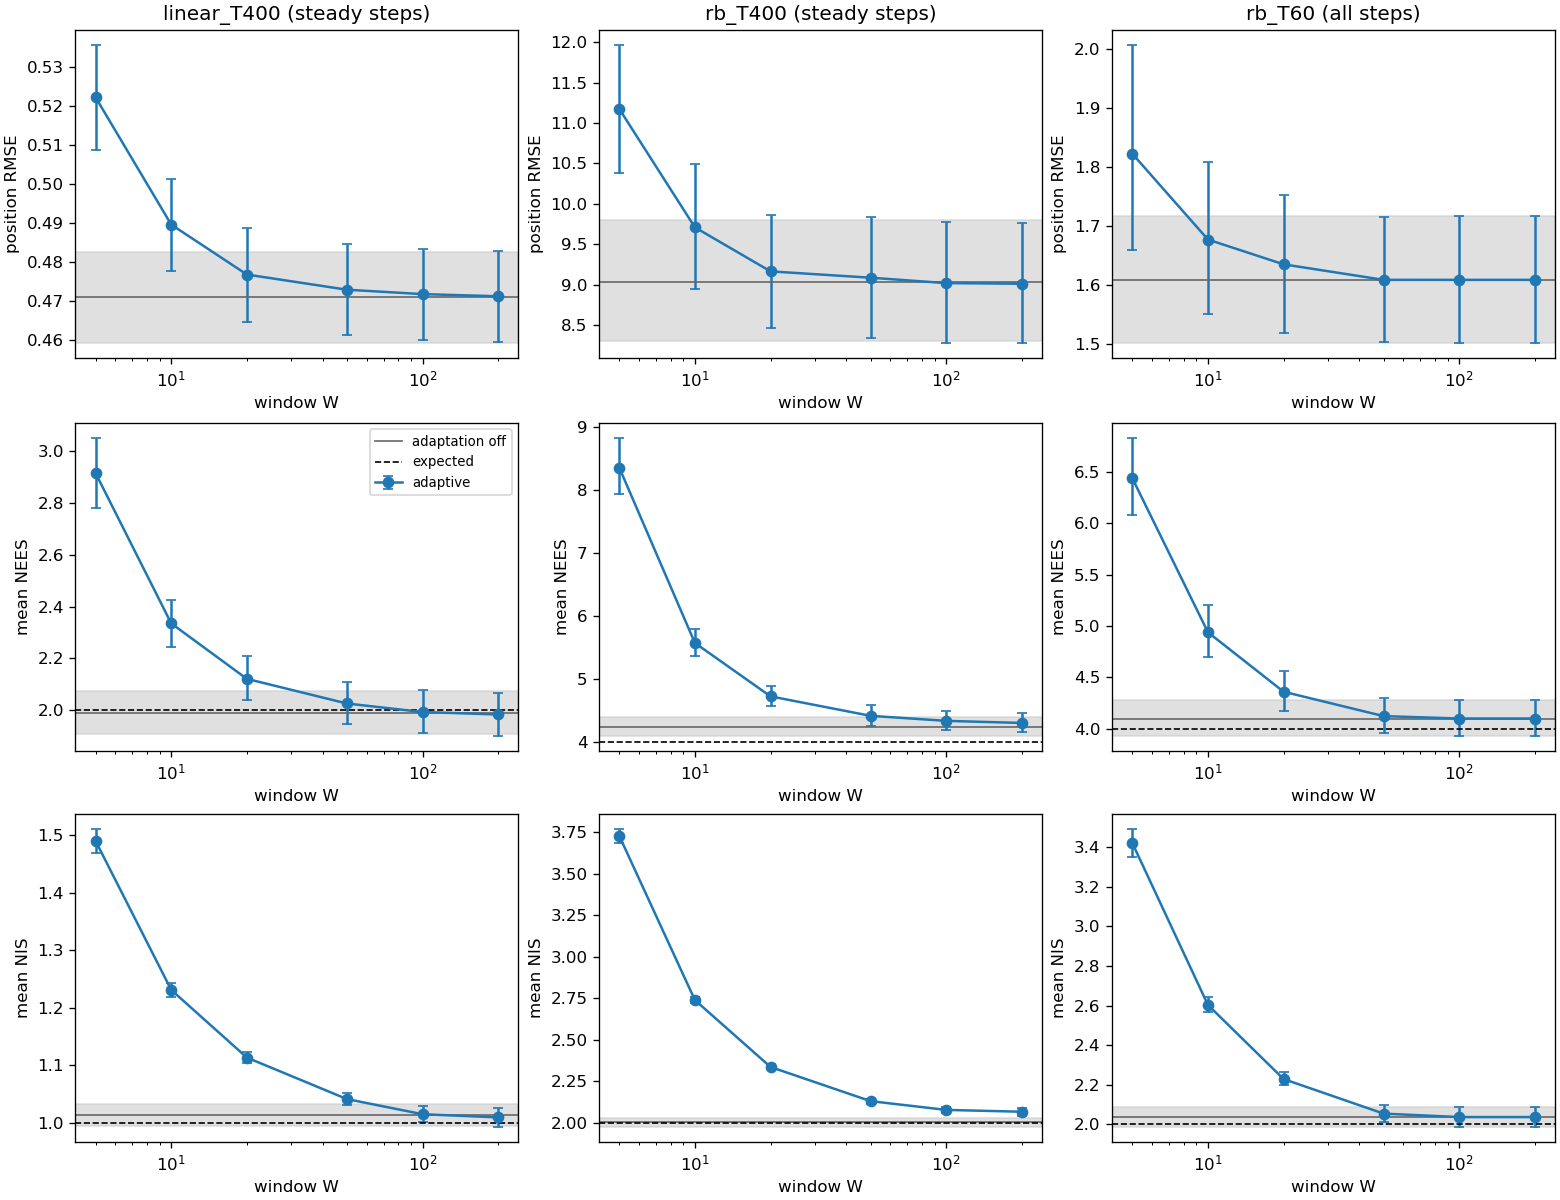
\includegraphics[width=0.85\linewidth]{filter_family/figures/adaptive_r_window.png}
\caption{Constant true $R$: RMSE, NEES and NIS of the adaptive filter versus the window, with the
non-adaptive filter as a band. Source: \texttt{experiments/filter\_family/figures/adaptive\_r\_window.png}.}\label{fig:adaptwindow}
\end{figure}

\paragraph{Time-varying noise.} With $R_{\mathrm{true}}(t)$ following a step, a ramp or bursts,
\obs{} every adaptive window has a lower NLL than the fixed nominal $R$, and no filter has a supported
advantage over the true-covariance filter in any of the \TVPairedTotal{} paired comparisons
(\TVPairedWorse{} are supported differences with a higher RMSE, NEES, NIS or NLL than the reference,
none with a lower one; Table~\ref{tab:main_tv}). The true-covariance filter
is a reference that knows $R$, not a performance bound. \obs{} The fixed-average filter, a hindsight
reference that uses the true mean of $R_{\mathrm{true}}(t)$ and is not available in practice, has a
lower NLL than every adaptive window on the burst patterns. \obs{} Short windows follow changes
quickly with large fluctuations, long windows are stable but lag (Figure~\ref{fig:tvburst}); the
window chosen on validation runs depends on the pattern. The window selection on validation runs and
the identifiability analysis (Table~\ref{tab:tv_ident}) are post-result amendments of that
benchmark.

\begin{table}[htbp]
\centering
\scriptsize
\caption{Time-varying measurement noise: mean innovation NLL for selected filters (all windows and RMSE/NEES in Tables~\ref{tab:tv_nll} and \ref{tab:tv_rmse}). The last row gives the window selected on validation runs (post-result amendment A3). Source: \path{experiments/filter_family/results/tv_r_summary.csv}.}\label{tab:main_tv}
\resizebox{\linewidth}{!}{%
\begin{tabular}{lllllll}
\toprule
Filter & lin. step & lin. ramp & lin. burst & rb step & rb ramp & rb burst \\
\midrule
fixed\_nominal & 3.68 & 3.67 & 2.66 & 3.63 & 3.62 & 1.77 \\
fixed\_average\_hindsight & 2.36 & 2.36 & 2.12 & 1.12 & 1.11 & 0.683 \\
true\_covariance & 2.10 & 2.29 & 1.71 & 0.617 & 0.983 & -0.146 \\
adaptive\_W5 & 2.27 & 2.45 & 2.17 & 1.30 & 1.61 & 1.28 \\
adaptive\_W20 & 2.16 & 2.32 & 2.20 & 0.801 & 1.09 & 0.990 \\
adaptive\_W200 & 2.33 & 2.59 & 2.41 & 1.10 & 1.57 & 1.27 \\
adaptive\_selected & 2.16 & 2.31 & 2.13 & 0.801 & 1.05 & 0.956 \\
selected window & 20 & 50 & 10 & 20 & 50 & 10 \\
\bottomrule
\end{tabular}}
\end{table}


\begin{figure}[htbp]\centering
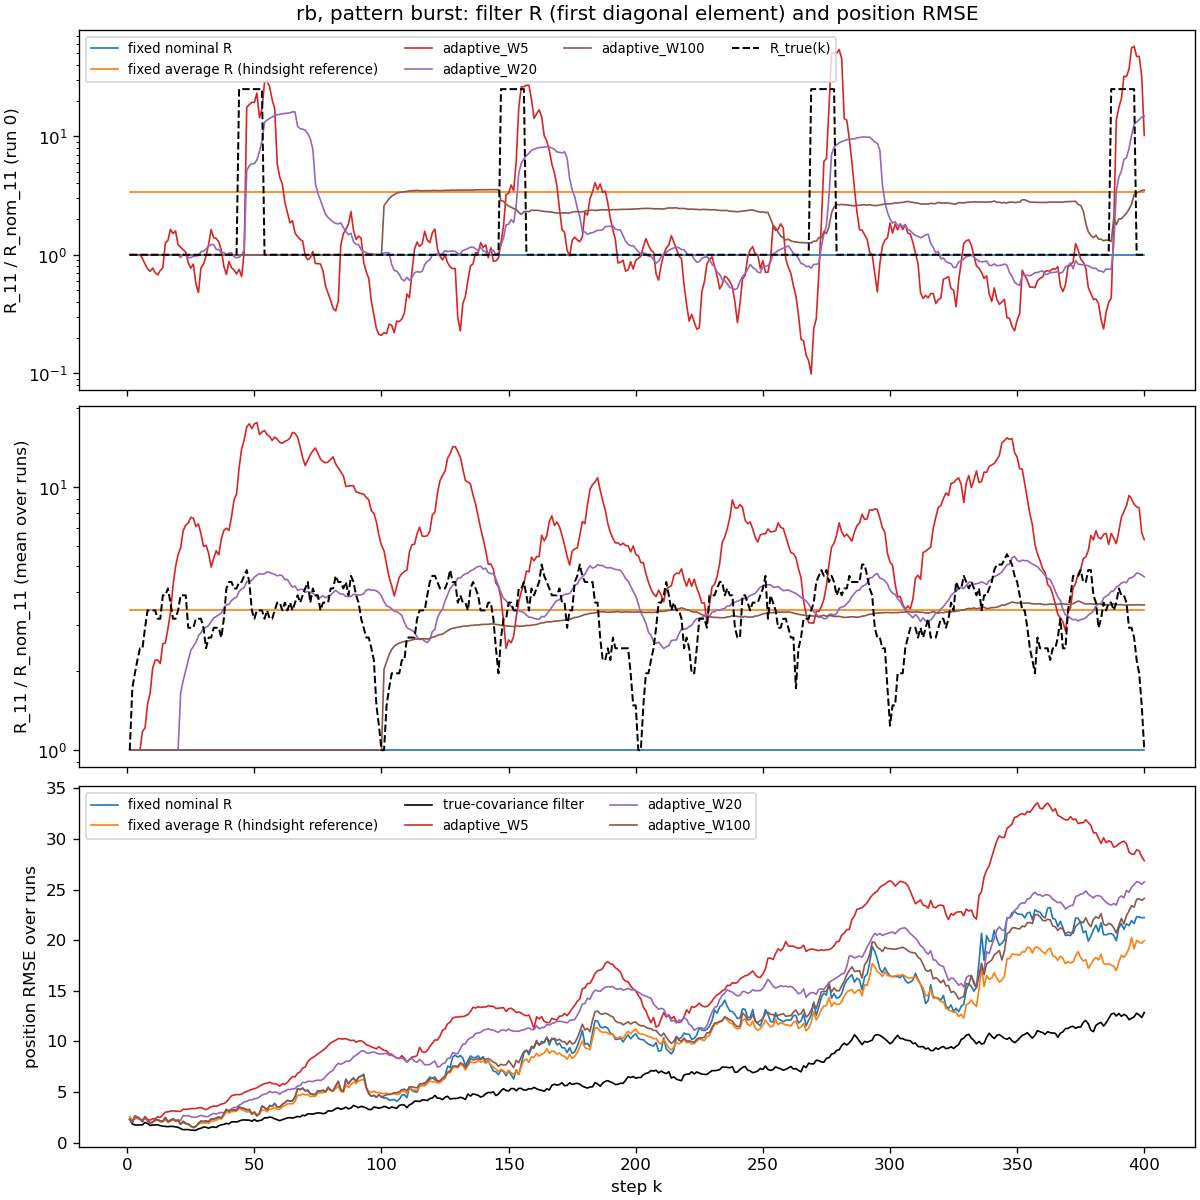
\includegraphics[width=0.8\linewidth]{filter_family/figures/tv_r_rb_burst.png}
\caption{Range-bearing, burst pattern: filter $R$ against $R_{\mathrm{true}}$ (run 0 and mean) and
RMSE over time. Source: \texttt{experiments/filter\_family/figures/tv\_r\_rb\_burst.png}.}\label{fig:tvburst}
\end{figure}

\subsection{The over-confidence mechanism of the $W=5$ window}\label{sec:mechanism}

\begin{table}[htbp]
\centering
\scriptsize
\caption{Over-confidence of the adaptive filter with $W = 5$ under constant true $R$: control runs, steady-state mean NEES differences; $^{\dagger}$ interval contains zero (W = 20 and 100 in Table~\ref{tab:ar_decomp}). Source: \texttt{experiments/neural\_r/results/diag\_decomposition.csv}.}\label{tab:main_decomp}
\resizebox{\linewidth}{!}{%
\begin{tabular}{lll}
\toprule
Term & Linear model & Range-bearing \\
\midrule
total: closed - off & 0.926 [0.837, 1.02] & 4.12 [3.73, 4.55] \\
feedback: closed - open\_replay & 0.475 [0.418, 0.538] & 2.38 [2.10, 2.71] \\
own-data correlation: open\_replay - indep\_open\_replay & 0.0516 [-0.0199, 0.122]$^{\dagger}$ & 0.170 [-0.0633, 0.402]$^{\dagger}$ \\
fluctuation: indep\_open\_replay - off & 0.399 [0.345, 0.453] & 1.57 [1.40, 1.74] \\
closed-loop statistics: indep\_closed\_replay - off & 0.794 [0.694, 0.898] & 3.73 [3.41, 4.08] \\
\bottomrule
\end{tabular}}
\end{table}


Control runs under constant $R_{\mathrm{true}}$ separate three hypotheses
(Table~\ref{tab:main_decomp}): the total excess NEES equals feedback (closed loop against the same
estimator on a frozen non-adaptive trajectory) plus own-data correlation (frozen-trajectory estimate
of the same run against that of another run) plus fluctuation (estimate of another run against the
true $R$). \obs{} (1) The spread of $\ln\hat R$ is high for short windows and decreases with $W$
(Table~\ref{tab:ar_spread}). \ver{} (2) Feedback through the post-fit residual raises the NEES
(linear model \DiagLinFiveFeedback). \ver{} (3) Fluctuations of the estimate alone, independent of
the current data and without feedback, raise the NEES through the gain (linear model
\DiagLinFiveFluct). \obs{} The own-data correlation term is not supported. \obs{} Replaying a
closed-loop $R$ sequence of another run reproduces \DiagLinFiveClosedStats{} of the linear-model
total \DiagLinFiveTotal: feedback acts mainly by enlarging the fluctuations of $\hat R$. \obs{} The
implemented post-fit estimate is never indefinite, whereas the innovation-form estimate is for short
windows (Table~\ref{tab:ar_psd}).

\subsection{The learned $R_t$ estimator: frozen primary experiment}\label{sec:learnedarch}

The design was frozen before training (\texttt{experiments/neural\_r/README.md}; SHA-256 and time
stamp in \texttt{DESIGN\_FREEZE.txt}). A GRU and, as a control without recurrent memory, an MLP on a
fixed window output a diagonal $R_t=\mathrm{diag}(\alpha_t)R_{\mathrm{base}}$ from causal innovation
features; the loss is the innovation NLL back-propagated through a differentiable linear KF that
reproduces the NumPy KF to rounding precision (test). The mathematical interface is given in
Section~\ref{sec:interface} and Figure~\ref{fig:diagram}. Each candidate and the adaptive baseline
had six configurations selected by validation NLL only (Table~\ref{tab:nr_train}); the gates were
fixed in advance (Table~\ref{tab:main_gates}).

\begin{table}[htbp]
\centering
\small
\caption{Gates fixed before training (details in Table~\ref{tab:nr_gates}). Source: \texttt{experiments/neural\_r/results/neural\_r\_gates.csv}.}\label{tab:main_gates}
\resizebox{\linewidth}{!}{%
\begin{tabular}{lll}
\toprule
Gate & Model & Outcome \\
\midrule
G1 & gru & passed \\
G2 & gru & passed (reported) \\
G3 & gru & failed \\
G4 & gru & evaluated \\
G5 & gru & evaluated \\
G1 & mlp & failed \\
G2 & mlp & passed (reported) \\
G3 & mlp & failed \\
G4 & mlp & evaluated \\
G5 & mlp & evaluated \\
G6 & gru vs mlp & evaluated \\
\bottomrule
\end{tabular}}
\end{table}


\subsection{Performance on held-out bursts}\label{sec:heldout}

\begin{table}[htbp]
\centering
\scriptsize
\caption{Bursts (in-distribution and held-out): mean innovation NLL and paired NLL difference of the learned models to the burst-selected adaptive window (gate G1 uses the two held-out sets). Source: \texttt{experiments/neural\_r/results/neural\_r\_summary.csv}, \texttt{experiments/neural\_r/results/neural\_r\_paired.csv}.}\label{tab:main_heldout}
\resizebox{\linewidth}{!}{%
\begin{tabular}{lllllll}
\toprule
Test set & true cov. & adaptive (burst sel.) & GRU & MLP & GRU $-$ adaptive & MLP $-$ adaptive \\
\midrule
burst & 1.71 & 2.13 & 1.93 & 2.00 & -0.206 [-0.225, -0.188] & -0.137 [-0.156, -0.121] \\
ho\_burst\_short & 1.60 & 2.22 & 1.93 & 1.96 & -0.291 [-0.328, -0.256] & -0.259 [-0.292, -0.227] \\
ho\_burst\_long & 2.17 & 2.58 & 2.48 & 2.69 & -0.106 [-0.126, -0.0888] & 0.109 [0.0906, 0.126] \\
\bottomrule
\end{tabular}}
\end{table}


\obs{} On both held-out burst sets the GRU has a lower NLL than the burst-selected adaptive window
(gate G1 passed for the GRU). \obs{} The MLP is lower on the short held-out bursts and higher on the
long ones (G1 failed for the MLP). \obs{} The true-covariance reference has a lower NLL than both
learned models on all burst sets (Table~\ref{tab:main_heldout}, Figure~\ref{fig:holong}). \obs{} The
GRU has a lower NLL than the MLP on every test set (G6), so recurrent memory beyond the fixed window
contributed under this budget.

\begin{figure}[htbp]\centering
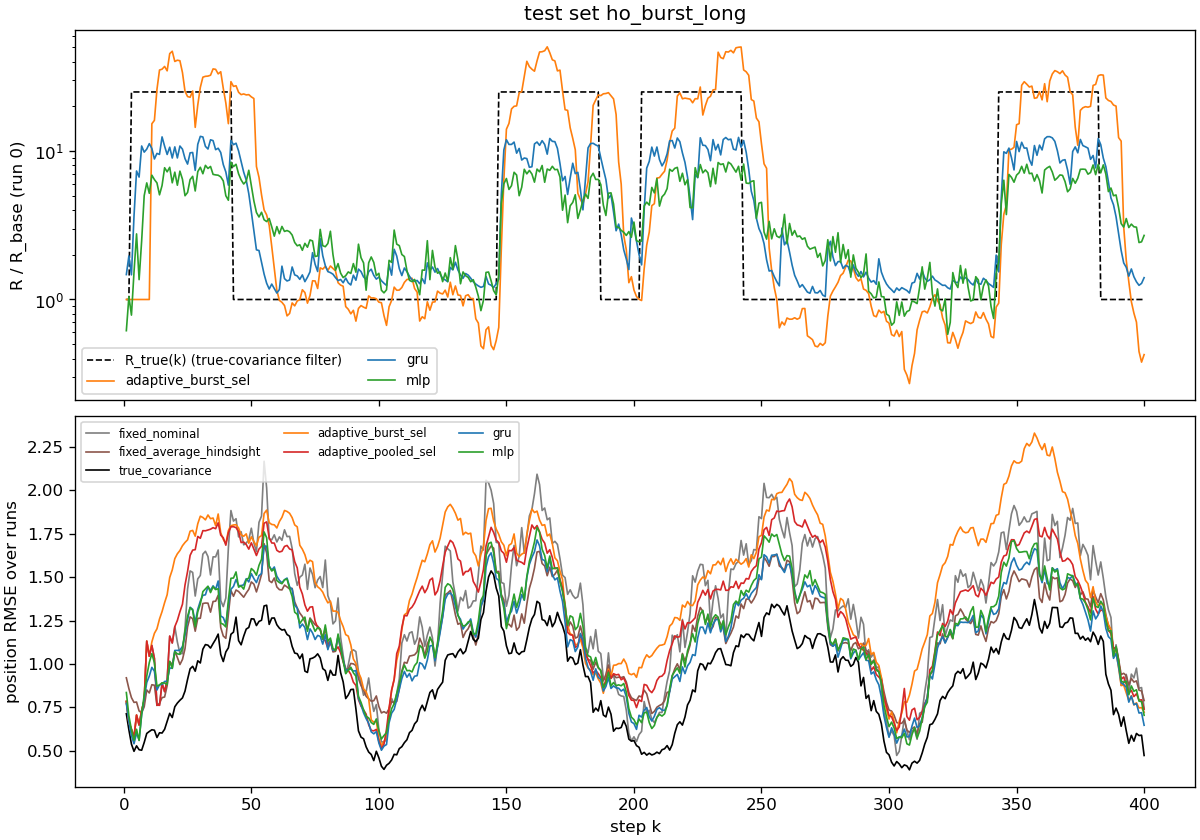
\includegraphics[width=0.8\linewidth]{neural_r/figures/eval_ho_burst_long.png}
\caption{Long held-out bursts: $R$ used by the true-covariance filter, the adaptive window, GRU and
MLP (run 0), and RMSE over runs. Source: \texttt{experiments/neural\_r/figures/eval\_ho\_burst\_long.png}.}\label{fig:holong}
\end{figure}

\subsection{Negative results and generalisation limits}\label{sec:negative}

\begin{table}[htbp]
\centering
\scriptsize
\caption{Negative results of the learned models: negative control with constant true $R$ (gate G3, against the non-adaptive filter), held-out step and ramp, and the tracking error on the long held-out bursts. Paired differences learned minus baseline. Source: \path{experiments/neural_r/results/neural_r_paired.csv}.}\label{tab:main_limits}
\resizebox{\linewidth}{!}{%
\begin{tabular}{lllll}
\toprule
Test set & Baseline & Metric & GRU & MLP \\
\midrule
constant & fixed\_nominal & pos\_rmse & 0.00297 [0.00164, 0.00432] & 0.0141 [0.0115, 0.0167] \\
constant & fixed\_nominal & mean\_nees & -0.124 [-0.137, -0.111] & -0.121 [-0.139, -0.103] \\
constant & fixed\_nominal & mean\_nis & -0.120 [-0.129, -0.110] & -0.171 [-0.180, -0.162] \\
constant & fixed\_nominal & mean\_nll & 0.0114 [0.0103, 0.0124] & 0.0325 [0.0304, 0.0346] \\
ho\_step & adaptive\_burst\_sel & mean\_nll & 0.0659 [0.0571, 0.0746] & 0.298 [0.286, 0.309] \\
ho\_step & adaptive\_burst\_sel & r\_abs\_logratio & 0.226 [0.217, 0.234] & 0.510 [0.503, 0.518] \\
ho\_ramp & adaptive\_burst\_sel & mean\_nll & 0.100 [0.0942, 0.106] & 0.338 [0.328, 0.349] \\
ho\_ramp & adaptive\_burst\_sel & r\_abs\_logratio & 0.232 [0.225, 0.239] & 0.558 [0.550, 0.565] \\
ho\_burst\_long & adaptive\_burst\_sel & r\_abs\_logratio & 0.0744 [0.0612, 0.0872] & 0.287 [0.276, 0.299] \\
\bottomrule
\end{tabular}}
\end{table}


\paragraph{Constant-$R$ control.} \obs{} Gate G3 failed for both models: with constant
$R_{\mathrm{true}}$ the learned filters have a higher RMSE and a lower NEES and NIS than the
non-adaptive filter, i.e.\ they are under-confident where no adaptation is needed
(Table~\ref{tab:main_limits}).

\paragraph{Held-out step and ramp.} \obs{} On the held-out step and ramp both learned models have a
higher NLL and a higher tracking error than the burst-selected adaptive window. Under G2 the GRU has
\GTwoGRU{} and the MLP \GTwoMLP{} cases in which its NEES or NIS is farther from the expected value
than that of a baseline; all are listed in \texttt{neural\_r\_g2\_cases.csv}, with the summary counts in
Table~\ref{tab:nr_worse}.

\paragraph{Saturation (post-result amendment 1).} This inspection was added after the results and
is kept apart from the frozen experiment; it uses forward passes of the saved models only.
\ver{} No explicit clamp exists, but the architecture bounds $\alpha_t$: the GRU hidden state lies in
$(-1,1)$, hence $\alpha_t\le\mathrm{softplus}(\sum|W|+b)+\varepsilon$, which is \BoundGRU{} for the
GRU (\BoundMLP{} for the MLP), and the attained maxima are close to it (Table~\ref{tab:nr_bound}).
\ver{} The bound does not coincide with the largest training factor, \TrainMaxFactor{}: at that factor
the GRU's median $\alpha$ on settled steps is \GRUalphaAtTwentyFive{} on the long held-out bursts and
\GRUalphaTrainTwentyFive{} on training batches (Figure~\ref{fig:sat}). \obs{} The GRU has a lower NLL
than the adaptive window on the long held-out bursts but a higher tracking error there
(Table~\ref{tab:main_limits}): \textbf{a lower predictive likelihood did not imply a better
calibrated covariance}. \hyp{} The bound reflects the end of the training budget (the GRU
validation NLL was still decreasing, Table~\ref{tab:nr_slopes}) or an NLL trade-off under uncertainty
about the end of a burst (\openlbl).

\begin{figure}[htbp]\centering
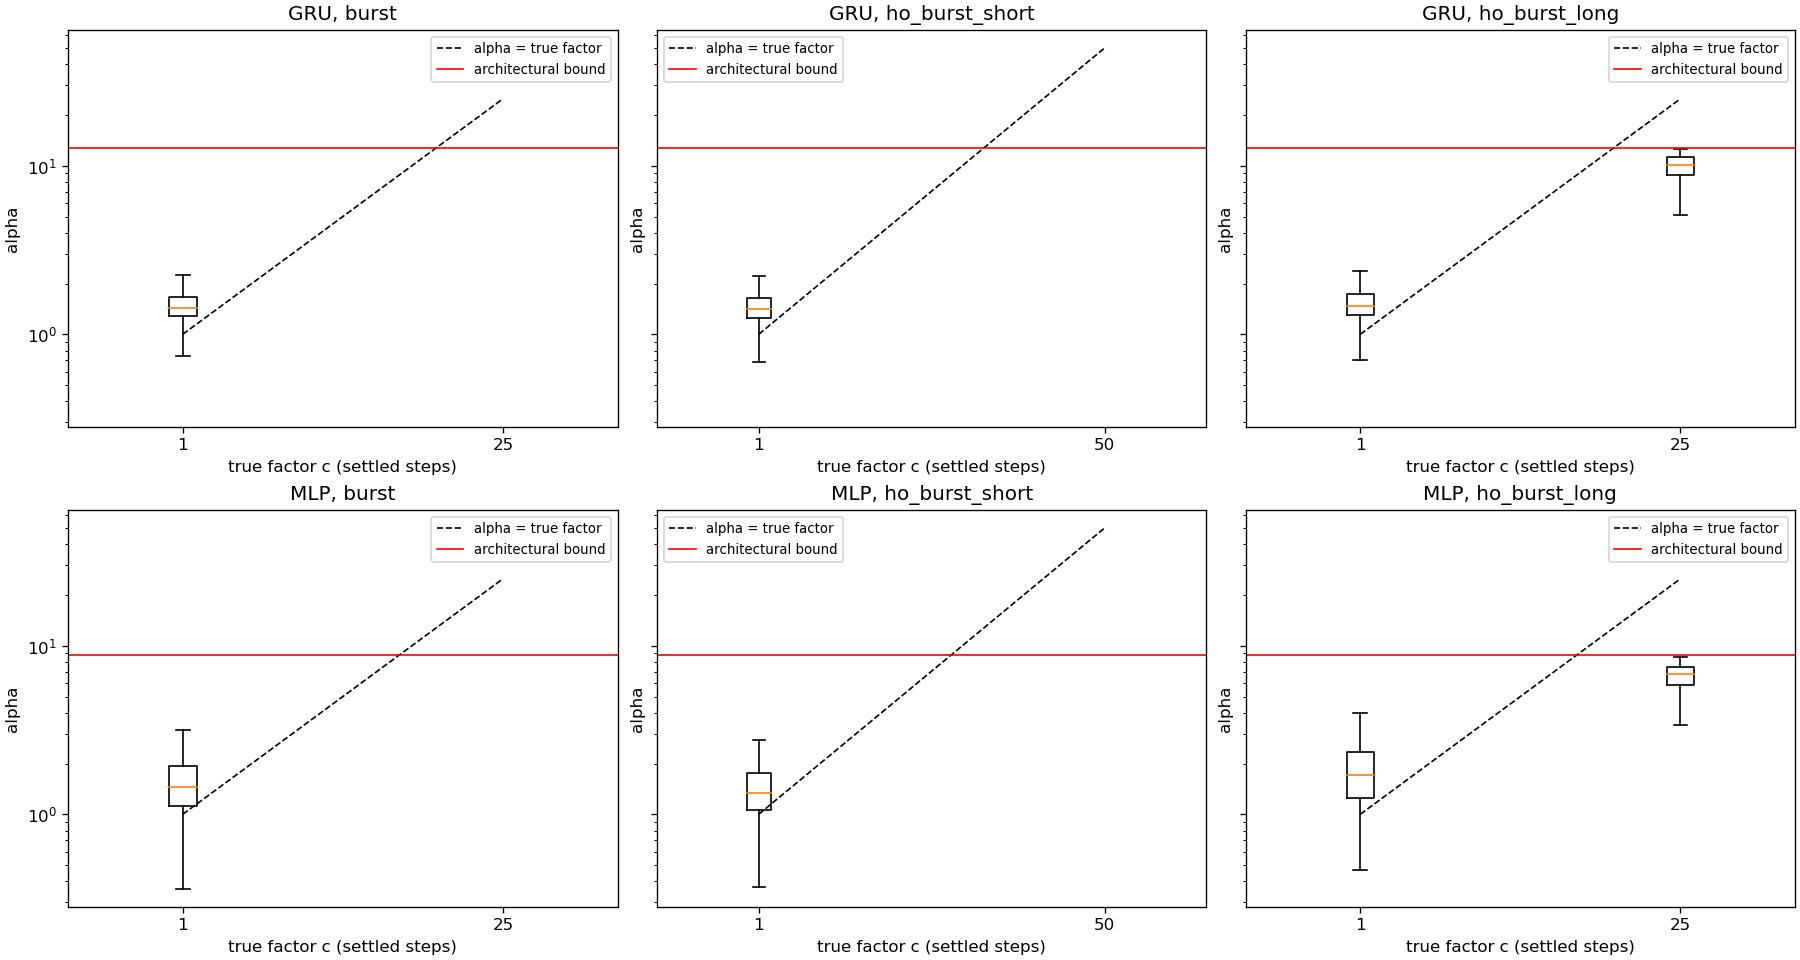
\includegraphics[width=0.8\linewidth]{neural_r/figures/saturation_alpha_vs_factor.png}
\caption{$\alpha_t$ versus the true factor on settled steps with the architectural bound. Source:
\texttt{experiments/neural\_r/figures/saturation\_alpha\_vs\_factor.png}.}\label{fig:sat}
\end{figure}

\paragraph{Structural mismatch: NIS versus NEES.}
\begin{table}[htbp]
\centering
\scriptsize
\caption{Structural IMU mismatch: paired change of the full-state NEES (expected 15) and of the mean NIS (expected 3) relative to the matched model. Source: \path{experiments/eskf_sensitivity/results/misalignment_paired.csv}, \path{experiments/eskf_sensitivity/results/scale_factor_paired.csv}.}\label{tab:main_mismatch}
\resizebox{\linewidth}{!}{%
\begin{tabular}{llll}
\toprule
Mismatch & Profile, scenario & $\Delta$ full NEES & $\Delta$ NIS \\
\midrule
misalignment 1.00\,deg & turning S0 & 1555 [1550, 1560] & 0.00437 [0.00289, 0.00585] \\
misalignment 3.00\,deg & turning S0 & 13987 [13973, 14001] & 0.0436 [0.0391, 0.0481] \\
misalignment 5.00\,deg & turning S0 & 38850 [38827, 38873] & 0.124 [0.117, 0.132] \\
scale factor 0.500\,\% & turning S0 & 8.97 [8.21, 9.74] & 0.00806 [0.00605, 0.0101] \\
scale factor 1.00\,\% & turning S0 & 33.9 [32.4, 35.5] & 0.0301 [0.0261, 0.0342] \\
scale factor 2.00\,\% & turning S0 & 132 [129, 135] & 0.117 [0.108, 0.125] \\
scale factor 0.500\,\% & turning S1 & 6.53 [5.75, 7.33] & 0.00316 [0.00163, 0.00467] \\
scale factor 1.00\,\% & turning S1 & 24.1 [22.5, 25.7] & 0.00954 [0.00649, 0.0126] \\
scale factor 2.00\,\% & turning S1 & 92.5 [89.1, 95.8] & 0.0319 [0.0259, 0.0380] \\
scale factor 0.500\,\% & aggressive S0 & 130 [127, 133] & 0.0441 [0.0400, 0.0485] \\
scale factor 1.00\,\% & aggressive S0 & 530 [524, 536] & 0.179 [0.171, 0.188] \\
scale factor 2.00\,\% & aggressive S0 & 2137 [2124, 2149] & 0.730 [0.713, 0.747] \\
scale factor 0.500\,\% & aggressive S1 & 111 [108, 114] & 0.0101 [0.00585, 0.0144] \\
scale factor 1.00\,\% & aggressive S1 & 453 [446, 459] & 0.0514 [0.0429, 0.0598] \\
scale factor 2.00\,\% & aggressive S1 & 1824 [1812, 1836] & 0.228 [0.211, 0.245] \\
\bottomrule
\end{tabular}}
\end{table}

\obs{} A fixed sensor-to-body misalignment and a gyroscope scale factor, with the filter otherwise
matched, raise the full-state NEES by up to orders of magnitude with supported differences, while the
mean NIS changes by at most \MisNISmaxchange{} (misalignment) and \SFNISmaxchange{} (scale factor)
(Table~\ref{tab:main_mismatch}). The innovation statistics, on which adaptive and learned
covariances are trained, therefore carry little signal of these errors.

\subsection{Lorenz benchmark of the KalmanNet paper}\label{sec:lorenz}

\paragraph{Reconstructed setup.} The Lorenz-attractor experiments of the paper \citep{revach2022}
(arXiv version 3, Section IV-D, Tables V and VII) were reconstructed from the paper and from the
reference code repository linked in it (\path{github.com/KalmanNet/KalmanNet_TSP}, commit
\texttt{828a2cf}). \textbf{The reference repository carries no licence; no KalmanNet source file was
copied into this repository}: the model was re-implemented from the equations, the shipped data file
was not used, and the reference code was only run from a temporary clone outside the repository.
The parameters and their sources (file and line of the reference commit) are listed in
\path{experiments/filter_family/README.md}: Lorenz dynamics discretised by a Taylor expansion of
order 5 with step 0.02, identity observation, $Q=q^2I$, $R=r^2I$ with $q^2/r^2=-20$\,dB, the paper's
grid of $1/r^2$, trajectories of 2000 steps, and the state-evolution mismatch in which the filters
use order 2. All filters of this repository receive the true $Q$ and $R$; nothing was tuned.

\begin{table}[htbp]
\centering
\scriptsize
\caption{Lorenz attractor: MSE [dB] of this study (true $Q$ and $R$, N = 100, T = 2000, $\nu = -20$\,dB) next to the EKF and UKF values transcribed from Tables V and VII of the paper (spread $10\log_{10}(\mathrm{std}+\mathrm{mean})-\mathrm{mean}$ where reported). Source: \path{experiments/filter_family/results/lorenz_comparison.csv}.}\label{tab:lorenz_comp}
\resizebox{\linewidth}{!}{%
\begin{tabular}{lllllll}
\toprule
Paper table & Setting & $1/r^2$ [dB] & Filter & Paper & This study [95\,\% CI] & Difference \\
\midrule
Table V & full & 0 & EKF & -10.45 & -10.44 [-10.50, -10.38] & 0.0109 \\
Table V & full & 10.0 & EKF & -20.37 & -20.47 [-20.51, -20.42] & -0.0968 \\
Table V & full & 20.0 & EKF & -30.40 & -30.48 [-30.53, -30.43] & -0.0806 \\
Table V & full & 30.0 & EKF & -40.39 & -40.47 [-40.52, -40.42] & -0.0799 \\
Table V & full & 40.0 & EKF & -49.89 & -50.41 [-50.47, -50.36] & -0.523 \\
Table V & full & 0 & UKF & -5.620 & -10.44 [-10.50, -10.38] & -4.82 \\
Table V & full & 10.0 & UKF & -12.04 & -20.47 [-20.51, -20.42] & -8.43 \\
Table V & full & 20.0 & UKF & -20.45 & -30.48 [-30.53, -30.43] & -10.0 \\
Table V & full & 30.0 & UKF & -30.05 & -40.47 [-40.52, -40.42] & -10.4 \\
Table V & full & 40.0 & UKF & -40.00 & -50.41 [-50.47, -50.36] & -10.4 \\
Table VII & full & 10.0 & EKF & -20.37 $\pm$ 0.25 & -20.47 [-20.51, -20.42] & -0.0968 \\
Table VII & full & 20.0 & EKF & -30.40 $\pm$ 0.24 & -30.48 [-30.53, -30.43] & -0.0806 \\
Table VII & full & 30.0 & EKF & -40.39 $\pm$ 0.24 & -40.47 [-40.52, -40.42] & -0.0799 \\
Table VII & full & 40.0 & EKF & -49.89 $\pm$ 0.20 & -50.41 [-50.47, -50.36] & -0.523 \\
Table VII & mismatch\_J2 & 10.0 & EKF & -19.47 $\pm$ 0.25 & -19.45 [-19.50, -19.39] & 0.0212 \\
Table VII & mismatch\_J2 & 20.0 & EKF & -23.63 $\pm$ 0.11 & -24.79 [-24.87, -24.71] & -1.16 \\
Table VII & mismatch\_J2 & 30.0 & EKF & -33.51 $\pm$ 0.18 & -25.87 [-25.98, -25.76] & 7.64 \\
Table VII & mismatch\_J2 & 40.0 & EKF & -41.15 $\pm$ 0.12 & -25.86 [-25.95, -25.77] & 15.3 \\
Table VII & mismatch\_J2 & 10.0 & UKF & -11.95 $\pm$ 0.87 & -19.45 [-19.50, -19.39] & -7.50 \\
Table VII & mismatch\_J2 & 20.0 & UKF & -20.45 $\pm$ 0.27 & -24.79 [-24.87, -24.71] & -4.34 \\
Table VII & mismatch\_J2 & 30.0 & UKF & -30.05 $\pm$ 0.090 & -25.87 [-25.98, -25.76] & 4.18 \\
Table VII & mismatch\_J2 & 40.0 & UKF & -39.98 $\pm$ 0.090 & -25.86 [-25.95, -25.77] & 14.1 \\
\bottomrule
\end{tabular}}
\end{table}


\paragraph{Agreement and disagreement.} \obs{} With full information our EKF agrees with the
paper's EKF within \LorEKFlowMaxAbsDiff\,dB from 0 to 30\,dB, inside the spread reported by the
paper; at 40\,dB it differs by \LorEKFhighDiff\,dB. \obs{} Our UKF equals our EKF to rounding,
while the paper's UKF has a higher MSE: the differences (this study minus paper) range from
\LorUKFdiffMin{} to \LorUKFdiffMax{} dB; this is a disagreement. \obs{} Under the J = 2 mismatch the filters of this repository level
off near \LorJtwoPlateau\,dB at high $1/r^2$, whereas the paper reports substantially lower values;
this is a disagreement. Only \LorInsideCount{} of the \LorCompTotal{} paper values lie inside our
bootstrap intervals (Table~\ref{tab:lorenz_comp}, Figure~\ref{fig:lorenz}). \obs{} The adaptive
filter loses the track under the mismatch at the highest $1/r^2$ (MSE \LorAdaptJtwoForty\,dB;
Table~\ref{tab:lorenz_summary}). Possible reasons, all \openlbl{} and untested: the paper's
model-based filters were tuned by a grid search over the filter $Q$, whose values are not reported;
the placement of the state-dependent matrix $A(x)$ differs between paper and code and changes the
discrete model from Taylor order two on; the paper's UKF is not part of the repository; the test-set
size and seeds are not stated; single versus double precision.

\begin{figure}[htbp]\centering
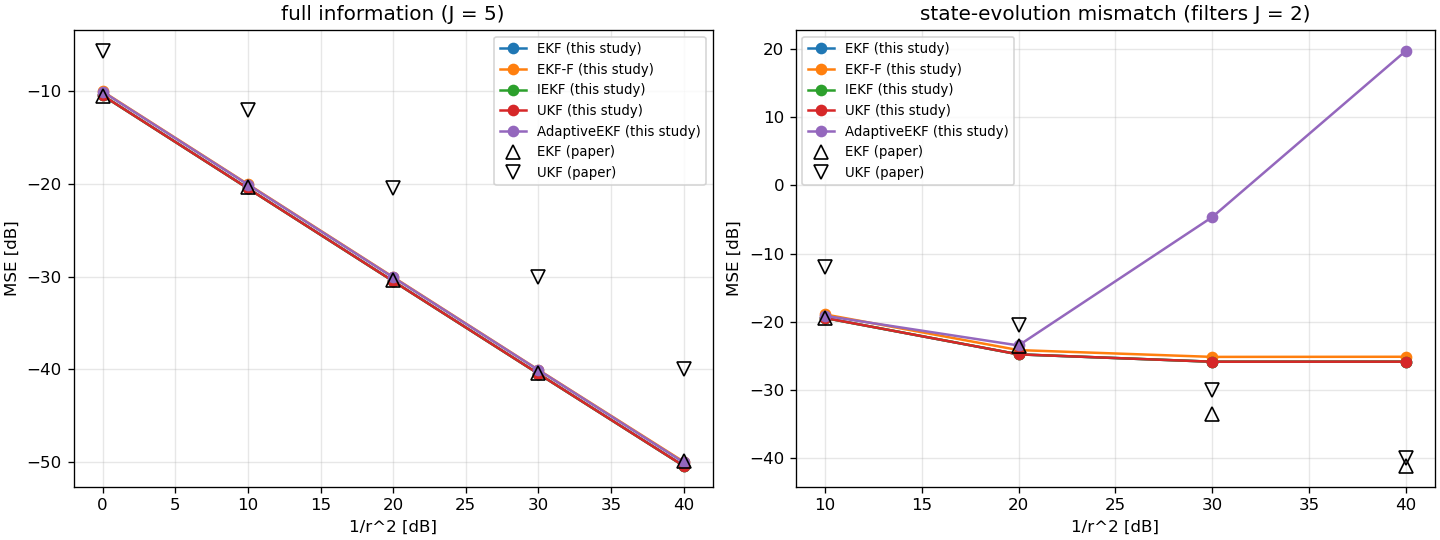
\includegraphics[width=0.9\linewidth]{filter_family/figures/lorenz_mse.png}
\caption{Lorenz attractor: MSE versus $1/r^2$ for the filters of this study, with the paper's EKF and
UKF values as markers; full information (left) and J = 2 mismatch (right). Source:
\path{experiments/filter_family/figures/lorenz_mse.png}.}\label{fig:lorenz}
\end{figure}

\paragraph{Exact Jacobian versus the reference EKF.} The reference code linearises the state
transition with $F(x)$ itself instead of the Jacobian of $F(x)\,x$. \ver{} On the test trajectories
exported from an exploratory run of the reference code, our EKF with that convention (EKF-F)
reproduces the reference EKF (\LorOurEKFF\,dB, spread \LorOurEKFFspread\,dB, against
\LorRefEKF\,dB and \LorRefEKFspread\,dB), which checks the re-implemented model against the code.
\obs{} The EKF with the exact Jacobian has a lower MSE (\LorOurEKF\,dB) and a mean NEES close to 3,
while EKF-F has a higher NEES (Table~\ref{tab:lorenz_knet}).

\begin{table}[htbp]
\centering
\scriptsize
\caption{Exploratory reference run (default Lorenz configuration of the reference code, full information, rotated observation, $1/r^2 = 10$\,dB, T = 100): reference-code results on its test set and the filters of this repository on the same exported trajectories and on an independent realisation. No KalmanNet result exists (training failed). Source: \path{experiments/filter_family/results/lorenz_knet_baseline.csv}.}\label{tab:lorenz_knet}
\resizebox{\linewidth}{!}{%
\begin{tabular}{lllllll}
\toprule
Source & Test data & Method & MSE [dB] & Spread [dB] & NEES & NIS \\
\midrule
reference repository & reference test set & EKF (reference code) & -19.66 & 1.31 & -- & -- \\
reference repository & reference test set & observation noise floor & -10.03 & 0.361 & -- & -- \\
this repository & same test trajectories (exported) & EKF & -20.31 [-20.49, -20.12] & 1.13 & 3.02 & 2.98 \\
this repository & same test trajectories (exported) & EKF-F & -19.66 [-19.87, -19.45] & 1.31 & 4.35 & 3.05 \\
this repository & same test trajectories (exported) & IEKF & -20.31 [-20.49, -20.12] & 1.13 & 3.02 & 2.98 \\
this repository & same test trajectories (exported) & UKF & -20.31 [-20.48, -20.12] & 1.12 & 3.02 & 2.98 \\
this repository & independent realisation (seed 0) & EKF & -20.42 [-20.59, -20.24] & 1.10 & 3.01 & 3.01 \\
this repository & independent realisation (seed 0) & EKF-F & -19.77 [-19.98, -19.55] & 1.33 & 4.34 & 3.08 \\
this repository & independent realisation (seed 0) & IEKF & -20.42 [-20.59, -20.24] & 1.10 & 3.01 & 3.01 \\
this repository & independent realisation (seed 0) & UKF & -20.42 [-20.59, -20.24] & 1.10 & 3.01 & 3.01 \\
\bottomrule
\end{tabular}}
\end{table}


\paragraph{KalmanNet runs (exploratory).} \obs{} The reference KalmanNet code, run with its default
Lorenz configuration (full information) and default hyperparameters, produced a finite training loss
only at the first step (\LorKnetFirstTrain\,dB) and non-finite losses afterwards; the run was stopped
after \LorKnetSteps{} logged steps, no checkpoint was saved and \textbf{no KalmanNet test result
exists}. KalmanNet outputs state estimates only, so NEES and NIS could not be computed for it in any
case. \ver{} A diagnosis on one training batch with the untrained network (Table~\ref{tab:lorenz_diag})
locates the first non-finite value in the forward pass: one trajectory's estimate grows to
\LorDiagState{} at step \LorDiagStep{}, and the Taylor term of order \LorDiagTaylor{} of the reference
state-transition function overflows single precision. \hyp{} The failed training run has the same
mechanism. No compatibility fix for the installed PyTorch (\LorDiagTorch) applies without changing
the model or the training, and an environment with the PyTorch version of the reference code could
not be created with the tools installed; whether that configuration trains there is \openlbl.

\subsection{Supporting evidence}\label{sec:support}

\paragraph{ESKF sensitivity and consistency.} \obs{} With the true parameters the full-state and all
sub-block NEES of the ESKF lie inside their bootstrap intervals around the expected values for three
profiles (Table~\ref{tab:es_consistency}); underestimated $R$ or $P_0$, disabled bias estimation,
long dropouts, ungated outliers, IMU spikes and a low measurement rate are among the settings with
supported effects (Tables~\ref{tab:es_closure}, \ref{tab:es_paired}). \ver{} The reset Jacobian and the
attitude columns of the transition matrix agree with finite differences (tests).

\paragraph{Structural mismatch.} \obs{} Against the true body attitude the attitude NEES under a
5-degree misalignment is far outside its interval; against the true sensor attitude, with the same
error definition and covariance block, it averages \AttRefSensorEarly{} over the first 10\,s and
\AttRefSensorLate{} over 30--60\,s (Table~\ref{tab:es_attref}). \hyp{} The early excess comes from the
initialisation around the body attitude (\openlbl). \obs{} Under a scale factor the change of the gyro-bias error has the
sign of the rate-equivalent error $s\,\bar\omega$ on \texttt{aggressive}, but not on the $z$ axis of
\texttt{turning} (Table~\ref{tab:es_sf_bias}); absorption as a mechanism is \openlbl.

\paragraph{GNSS scenarios S0, S1, S2.} \obs{} With a matched model the full NEES stays near its
expected value inside and outside the outage and the RMS position error grows below the $3\sigma$
bound; with misalignment the error after the outage grows with the angle, and under a 2\,\% scale
factor on \texttt{aggressive} it exceeds $3\sigma$ late in the outage (Tables~\ref{tab:es_gnss},
\ref{tab:es_drift}, Figure~\ref{fig:sfagg}).

\paragraph{Real data.}
\begin{table}[htbp]
\centering
\scriptsize
\caption{Real sequences compared with the synthetic profiles (full characterisation in Table~\ref{tab:ds_summary}). Source: \path{analysis/dataset_char/results/summary.csv}, \path{analysis/dataset_char/results/synthetic_profiles.csv}.}\label{tab:main_ds}
\resizebox{\linewidth}{!}{%
\begin{tabular}{lll}
\toprule
Quantity & KITTI drive 0016 & EuRoC V1\_01\_easy \\
\midrule
Measured IMU rate [Hz] & 100 & 200 \\
Longest static segment [s] & 0 & 0 \\
Noise density, bias instability & not identifiable & not identifiable \\
Speed median / max [m/s] & 13.7 / 15.7 & 0.397 / 1.06 \\
$|\omega|$ median / max [rad/s] & 0.0152 / 0.0899 & 0.231 / 0.938 \\
Fraction of time turning & 0 & 0.844 \\
synthetic \texttt{straight}: speed max, $|\omega|$ max, turning & 4.00, 0, 0 &  \\
synthetic \texttt{turning}: speed max, $|\omega|$ max, turning & 5.92, 0.664, 0.822 &  \\
synthetic \texttt{aggressive}: speed max, $|\omega|$ max, turning & 4.93, 4.10, 1.00 &  \\
\bottomrule
\end{tabular}}
\end{table}

The characterisation relates the synthetic profiles to real motion and identifies what the data
cannot determine; it is not a validation of the filters. \obs{} KITTI drives at nearly constant speed
with angular rates below the turning threshold, closest to \texttt{straight} but several times
faster; EuRoC rotates most of the time at low speed, closest to \texttt{turning} in rotation but much
slower (Table~\ref{tab:main_ds}, Figure~\ref{fig:motion}). \obs{} Neither sequence has a static
segment, so noise densities, bias instability and bias random walk are not identifiable; the KITTI
inertial data come from an integrated GPS/inertial unit whose ground truth is its own navigation
solution, and the EuRoC ground truth is a batch estimate that uses the IMU (Appendix~\ref{app:data}).

%==================================================================================================
\section{Which component to learn, and the interface of the learned estimator}\label{sec:which}
%==================================================================================================

\paragraph{Evidence.} \obs{} With a correct model and the true parameters the linear KF and the ESKF
are consistent; mis-specified covariances degrade the estimates through ratios only
(Proposition~\ref{prop:scale}). \obs{} When the measurement noise is nonstationary, adapting $R$
improves the NLL over a fixed $R$, and the GRU estimate improved it further on bursts, including
held-out bursts; it failed the constant-$R$ control, generalised worse to held-out steps and ramps and
saturated below the largest factor of its training data. \obs{} Structural IMU errors raise the NEES while
leaving the NIS nearly unchanged. \hyp{} An innovation-driven adaptation or learned $R_t$ therefore
would not detect such errors; this has not been tested, because no adaptive or learned ESKF was run
(\openlbl). The evidence supports learning or adapting $R_t$ only for genuinely nonstationary
measurement noise, with calibration gates as part of the acceptance, and not as a remedy for IMU
model errors, which require explicit states or calibration.

\paragraph{Mathematical interface (as implemented)}\label{sec:interface}
for the linear model with $m=1$, $R_{\mathrm{base}}$ the nominal $R$.
\begin{itemize}
\item \emph{Causal inputs.} After the update at step $j$ the feature vector is
\begin{equation}\label{eq:features}
\phi_j=\Big[\,\frac{\nu_j}{\sqrt{R_{\mathrm{base}}}},\ \frac{\nu_j}{\sqrt{S_j}},\ \ln\frac{S_j}{R_{\mathrm{base}}}\,\Big],
\end{equation}
with $\nu_j$ the innovation and $S_j$ its covariance. The GRU uses $h_t=\mathrm{GRU}(\phi_{t-1},h_{t-1})$
with $\phi_0=0$, $h_0=0$ (hidden size 16); the MLP uses
$[\phi_{t-20},\dots,\phi_{t-1}]$, zero-padded, with two tanh layers of 32 units.
$R_{\mathrm{true}}$ is never an input and never a label.
\item \emph{Covariance parameterisation.} $\alpha_t=\mathrm{softplus}(w\tp h_t+b)+\varepsilon$,
$\varepsilon=10^{-3}$, $R_t=\mathrm{diag}(\alpha_t)\,R_{\mathrm{base}}$; since $\alpha_t\ge\varepsilon>0$
and $R_{\mathrm{base}}\succ0$ is diagonal, $R_t\succ0$ by construction. The output bias is
initialised so that $\alpha_t\approx1$.
\item \emph{Entry into the Kalman update.} At step $t$: prediction
$\hat x^-_t=F\hat x_{t-1}$, $P^-_t=FP_{t-1}F\tp+Q$; then $R_t$ from the history up to $t-1$; then
$S_t=HP^-_tH\tp+R_t$, $K_t=P^-_tH\tp S_t^{-1}$, $\hat x_t=\hat x^-_t+K_t\nu_t$ and the Joseph update
$P_t=(I-K_tH)P^-_t(I-K_tH)\tp+K_tR_tK_t\tp$; finally $\phi_t$ is formed.
\item \emph{Training objective.} The mean of the innovation NLL~\eqref{eq:nll} over steps and
trajectories, back-propagated through the full recursion (400 steps, no truncation), Adam with
gradient clipping; the checkpoint with the lowest pooled validation NLL is kept.
\item \emph{Training versus inference.} In training, gradients flow through $R_t$, $S_t$, $K_t$ and
the state recursion; in inference the parameters are fixed and the same causal recursion runs
without gradients. $R_{\mathrm{true}}$ enters only the evaluation metrics (tracking error) and the
true-covariance reference.
\item \emph{GRU versus MLP control.} Same features, parameterisation, loss and budget; the MLP sees
only a fixed 20-step window, so a difference isolates recurrent memory (gate G6).
\end{itemize}

\begin{figure}[htbp]\centering
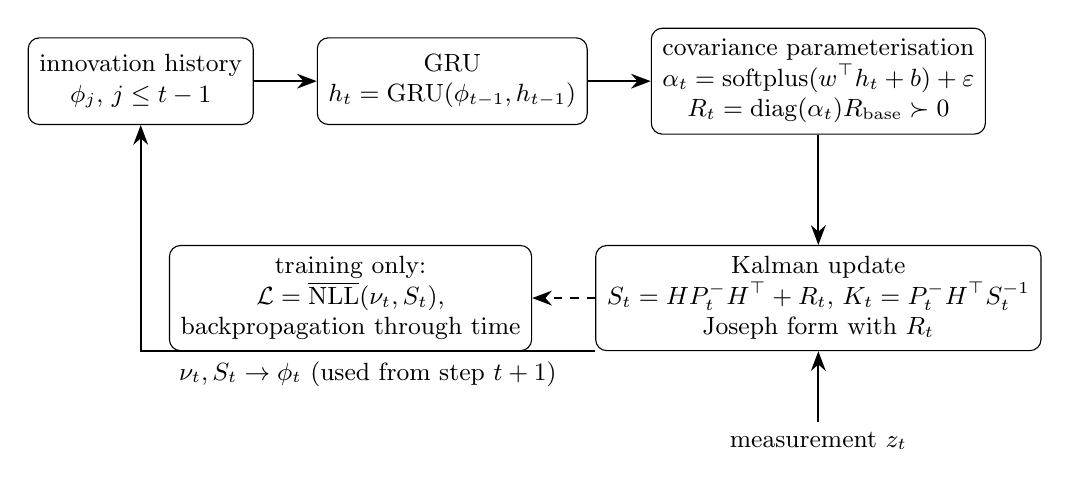
\begin{tikzpicture}[node distance=1.0cm and 0.8cm, every node/.style={font=\small},
  box/.style={draw, rounded corners, align=center, minimum height=1.1cm, inner sep=4pt},
  arr/.style={-{Stealth[length=2.5mm]}, thick}]
\node[box] (hist) {innovation history\\$\phi_j$, $j\le t-1$};
\node[box, right=of hist] (gru) {GRU\\$h_t=\mathrm{GRU}(\phi_{t-1},h_{t-1})$};
\node[box, right=of gru] (par) {covariance parameterisation\\$\alpha_t=\mathrm{softplus}(w\tp h_t+b)+\varepsilon$\\$R_t=\mathrm{diag}(\alpha_t)R_{\mathrm{base}}\succ0$};
\node[box, below=1.4cm of par] (kf) {Kalman update\\$S_t=HP^-_tH\tp+R_t$, $K_t=P^-_tH\tp S_t^{-1}$\\Joseph form with $R_t$};
\node[box, left=of kf] (loss) {training only:\\$\mathcal L=\overline{\mathrm{NLL}}(\nu_t,S_t)$,\\backpropagation through time};
\node[below=0.9cm of kf, align=center] (z) {measurement $z_t$};
\draw[arr] (hist) -- (gru);
\draw[arr] (gru) -- (par);
\draw[arr] (par) -- (kf);
\draw[arr] (z) -- (kf);
\draw[arr, dashed] (kf) -- (loss);
\draw[arr] (kf.south west) -| node[pos=0.25, below]{$\nu_t,S_t\rightarrow\phi_t$ (used from step $t+1$)} (hist.south);
\end{tikzpicture}
\caption{Interface of the learned covariance estimator as implemented (GRU candidate; the MLP
replaces the GRU by a fixed-window network). $R_{\mathrm{true}}$ is neither an input nor a
label.}\label{fig:diagram}
\end{figure}

%==================================================================================================
\section{Limitations and next steps}\label{sec:limits}
%==================================================================================================

\paragraph{Limitations.}
(i) \emph{Model-matched synthetic validation}: the filters are evaluated on data from their own model
family with one property changed at a time. (ii) \emph{Single real sequences}: one KITTI and one
EuRoC sequence, without static segments. (iii) \emph{Small $N$}: between 30 and 200 runs per
setting; intervals are wide for heavy-tailed quantities. (iv) \emph{Non-independent ground truth}:
the KITTI reference is the unit's own navigation solution and the EuRoC estimate uses the IMU.
(v) \emph{Unverified explanations}: statements labelled \hyp{} and Appendix~\ref{app:open}.
(vi) \emph{Linear-model-only prototype}: the learned $R_t$ was trained and evaluated on the linear
model only and is not integrated into the ESKF. (vii) \emph{No KalmanNet comparison}: the reference
KalmanNet code did not train in the available environment, and the reconstruction of the paper's
Lorenz setting contains ambiguities (form of $A(x)$, tuned filter $Q$, UKF settings).

\paragraph{Next steps.}
(1) Run the adaptive and the learned $R_t$ inside the ESKF under misalignment and scale factor, to
test the hypothesis of Section~\ref{sec:which}. (2) Repeat the learned-$R_t$ protocol on the
range-bearing benchmark, and address the bound on $\alpha_t$ in a new pre-registered design, without
changing the existing results. (3) Run the attitude-reference control initialised around the sensor
attitude. (4) Obtain static IMU recordings for an Allan analysis \citep{allan1966} and evaluate on
several sequences per dataset. (5) Resolve the open citation items and the match of the implemented
adaptive rule with the cited estimator. (6) Create an environment with the PyTorch version of the
reference KalmanNet code (an older Python and an environment manager are needed) and repeat the
exploratory run; any change of precision or initialisation would be a separate, pre-registered
amendment.

\bibliographystyle{plainnat}
\bibliography{refs}

%==================================================================================================
\clearpage
\appendix
\section{Detailed equations of all approaches}\label{app:equations}
%==================================================================================================

\paragraph{KF.} $\hat x^-_k=F\hat x_{k-1}$, $P^-_k=FP_{k-1}F\tp+Q$, $S_k=HP^-_kH\tp+R$,
$K_k=P^-_kH\tp S_k^{-1}$, $\hat x_k=\hat x^-_k+K_k(z_k-H\hat x^-_k)$,
$P_k=(I-K_kH)P^-_k(I-K_kH)\tp+K_kRK_k\tp$ \citep{kalman1960}. Cost $O(n^3+m^3)$.

\paragraph{Information filter.} With $Y=P^{-1}$, $y=P^{-1}\hat x$: update
$Y_k=Y^-_k+H\tp R^{-1}H$, $y_k=y^-_k+H\tp R^{-1}z_k$; the prediction requires
$Y^-_k=(FY_{k-1}^{-1}F\tp+Q)^{-1}$ or an equivalent form \citep{barshalom2001}.

\paragraph{Square-root forms.} Propagate $L$ with $P=LL\tp$ (or $UDU\tp$) through orthogonal
transformations of the stacked factors of $FPF\tp+Q$ and of the update, preserving symmetry and
positive definiteness under rounding \citep{bierman1977}.

\paragraph{EKF.} $\hat x^-_k=f(\hat x_{k-1})$, $F_k=\partial f/\partial x|_{\hat x_{k-1}}$,
$P^-_k=F_kP_{k-1}F_k\tp+Q$; $H_k=\partial h/\partial x|_{\hat x^-_k}$, $\nu_k=z_k-h(\hat x^-_k)$ (with
angle wrapping where needed), followed by the Joseph update with $H_k$.

\paragraph{IEKF.} From $x_0=\hat x^-$ iterate $H_i=H(x_i)$,
$r_i=z-h(x_i)-H_i(\hat x^--x_i)$, $K_i=P^-H_i\tp(H_iP^-H_i\tp+R)^{-1}$, $x_{i+1}=\hat x^-+K_ir_i$ until
$\|x_{i+1}-x_i\|\le\mathrm{tol}$; the covariance uses the last $K_i$, $H_i$ \citep{bell1993}. The
reported innovation and $S$ are those at the prior.

\paragraph{ESKF.} Nominal propagation with $\omega_i=\omega_{m,i}-b_g$,
$\phi=\tfrac{\Delta t}{2}(\omega_0+\omega_1)+\tfrac{\Delta t^2}{12}(\omega_0\times\omega_1)$,
$q_1=q_0\otimes\mathrm{Exp}(\phi)$, $a_i=R(q_i)(f_{m,i}-b_a)+g$,
$p_1=p_0+v_0\Delta t+\Delta t^2(a_0/3+a_1/6)$, $v_1=v_0+\tfrac{\Delta t}{2}(a_0+a_1)$. Error dynamics
as in Section~\ref{sec:family} with non-zero blocks $A_{p,v}=I$, $A_{v,\theta}=-R[\tilde f]_\times$,
$A_{v,b_a}=-R$, $A_{\theta,\theta}=-[\tilde\omega]_\times$, $A_{\theta,b_g}=-I$;
$Q_d=\mathrm{diag}(0,\sigma_a^2\Delta t I,\sigma_g^2\Delta t I,\sigma_{bg}^2\Delta t I,\sigma_{ba}^2\Delta t I)$;
optional innovation gate on $\chi^2_3$. Injection $p\mathrel{+}=\delta p$, $v\mathrel{+}=\delta v$,
$q\leftarrow q\otimes\mathrm{Exp}(\delta\theta)$, $b\mathrel{+}=\delta b$, then the reset
$P\leftarrow GPG\tp$ \citep{sola2017}.

\paragraph{UKF.} $\lambda=\alpha^2(n+\kappa)-n$; sigma points $\hat x$, $\hat x\pm\sqrt{n+\lambda}\,L_i$;
weights $W^m_0=\lambda/(n+\lambda)$, $W^c_0=W^m_0+1-\alpha^2+\beta$, $W^m_i=W^c_i=1/(2(n+\lambda))$;
$S=\sum W^c_i(Z_i-\hat z)(Z_i-\hat z)\tp+R$, $P_{xz}=\sum W^c_i(X_i-\hat x)(Z_i-\hat z)\tp$,
$K=P_{xz}S^{-1}$, $P\leftarrow P-KSK\tp$ \citep{julier2004}. The implementation uses $\alpha=1$,
$\beta=2$, $\kappa=0$ and a circular mean for the bearing. Reference for the scaled transform:
\todo{citation needed: scaled unscented transformation}.

\paragraph{CKF.} Points $\hat x\pm\sqrt n\,L_i$, $i=1,\dots,n$, weights $1/(2n)$
\citep{arasaratnam2009}.

\paragraph{Invariant EKF.} For a state on a matrix Lie group $\chi$ and group-affine dynamics, the
right- or left-invariant error $\eta=\hat\chi\chi^{-1}$ (or $\chi^{-1}\hat\chi$) satisfies an
autonomous error equation, whose linearisation $\xi$ with $\eta=\exp(\xi^\wedge)$ is used in the
filter \citep{barrau2017}.

\paragraph{Ensemble KF.} Ensemble $\{x^{(i)}\}$, sample covariance $\hat P$, update with
$K=\hat PH\tp(H\hat PH\tp+R)^{-1}$ applied to each member with perturbed observations
\citep{evensen1994}.

\paragraph{Particle filter.} Propagate $x^{(i)}_k\sim p(x_k|x^{(i)}_{k-1})$, weight
$w^{(i)}\propto w^{(i)}p(z_k|x^{(i)}_k)$, resample when the effective sample size is small
\citep{gordon1993}.

\paragraph{Adaptive estimates.} Residual-based (implemented),
\begin{equation}\label{eq:adaptive}
\hat R_{k+1}=\frac1W\sum_{j=k-W+1}^{k}e_je_j\tp+H(\hat x^+_k)P^+_kH(\hat x^+_k)\tp,\qquad e_j=z_j-h(\hat x^+_j),
\end{equation}
from $\Ex[ee\tp]=R-HP^+H\tp$ for an optimal linear filter; innovation-based (diagnostic only),
$\hat R=\frac1W\sum\nu_j\nu_j\tp-HP^-H\tp$, from $\Ex[\nu\nu\tp]=HP^-H\tp+R$
\citep{mehra1970,mohamed1999}. Whether the implemented rule matches the cited estimator exactly is
\openlbl.

\paragraph{Learned variants.} Learned $R_t$: Section~\ref{sec:interface}. Learned gain: a recurrent
network maps innovation features to $K_t$ \citep{revach2022}. Learned noise covariances through a
differentiable filter: \citep{haarnoja2016}; learned $R_t$ from sensor data in navigation:
\todo{citation needed: learned measurement covariance in visual-inertial or GNSS/INS filtering}.

%==================================================================================================
\section{Proof of the common-scale identity}\label{app:proof}
%==================================================================================================
\begin{proof}[Proof of Proposition~\ref{prop:scale}]
Let $P^{(c)}$ be the covariances of the filter run with $(cQ,cR,cP_0)$ and assume
$P^{(c)}_{k-1}=cP_{k-1}$, which holds for $k-1=0$. Then
$P^{-(c)}_k=F\,cP_{k-1}F\tp+cQ=cP^-_k$ and $S^{(c)}_k=H\,cP^-_kH\tp+cR=cS_k$, so
$K^{(c)}_k=cP^-_kH\tp(cS_k)^{-1}=K_k$. With equal gains and equal initial means, estimates and
innovations coincide at every step. The Joseph update gives
$P^{(c)}_k=(I-K_kH)\,cP^-_k(I-K_kH)\tp+K_k\,cR\,K_k\tp=cP_k$, which completes the induction. Hence
$e\tp(cP)^{-1}e=\mathrm{NEES}/c$ and $\nu\tp(cS)^{-1}\nu=\mathrm{NIS}/c$. The innovation NLL changes by
$\tfrac12(1/c-1)\,\mathrm{NIS}+\tfrac m2\ln c$.
\end{proof}
The identity is tested in \texttt{test\_common\_scale\_invariance} and visible in
Table~\ref{tab:lin_scale}.

%==================================================================================================
\section{Parameter grids}\label{app:grids}
%==================================================================================================
Quoted from the protocol sections of the READMEs.
\begin{itemize}
\item \textbf{Linear KF}: scale $s\in\mathrm{logspace}(-3,3,13)$ of $Q$, $R$ or $P_0$; $N=200$, $T=200$;
ratio study with $T=2000$ (steady state $k\ge1000$) and a $13\times13$ grid of $Q$ and $R$ scales.
\item \textbf{Range-bearing}: $N=100$, 60 steps; $s\in\mathrm{logspace}(-2,2,9)$ for $Q$, $R$, $P_0$;
bearing noise 0.005--0.5\,rad; initial position standard deviation 0.5--40\,m; closest approach
1--100\,m; adaptive window 20.
\item \textbf{ESKF sweeps}: \texttt{turning}, 60\,s, IMU 200\,Hz, position 10\,Hz, $N=30$;
$s\in\mathrm{logspace}(-2,2,7)$ for IMU noise, bias random walk, $R$, $P_0$; bias scale 0--10 with
and without bias estimation; dropout 0--40\,s from 15\,s; outlier probability 0--0.2 with gate off
and on (threshold at probability 0.999); IMU spike probability 0--0.01; profile; measurement rate
1--20\,Hz. Consistency study $N=50$ on three profiles with and without reset.
\item \textbf{Mismatch and GNSS}: misalignment 0, 1, 3, 5\,deg about body $x$; gyroscope scale factor
0, 0.5, 1, 2\,\% on \texttt{turning} and \texttt{aggressive}; S0 (10\,Hz), S1 (outage from 20\,s),
S2 (no position); $N=50$ paired runs.
\item \textbf{Adaptive $R$}: windows 5, 10, 20, 50, 100, 200; constant $R$ on the linear model and
range-bearing ($T=400$ and 60); patterns step ($\times10$ at mid-run), ramp (1 to 10), bursts
($\times25$, four of 10 steps); $N=100$; validation seeds for window selection (amendment A3).
\item \textbf{Learned $R_t$}: training patterns burst 40\,\%, step 20\,\%, ramp 20\,\%, constant 20\,\%;
six configurations per candidate (learning rate $\{10^{-3},3\cdot10^{-3},10^{-2}\}\times$ weight decay
$\{0,10^{-4}\}$); batch 32, 400 iterations; test sets constant, step, ramp, burst and held-out step,
ramp, short and long bursts and sine; recovery threshold a factor of two.
\item \textbf{Real data}: static criterion (1\,s window, $|\omega|$ standard deviation below
0.01\,rad/s, $|f|$ below 0.05\,m/s$^2$, speed below 0.05\,m/s), minimum static length 10\,s, spike
criterion 6 robust scales from an 11-sample running median, turning threshold 0.1\,rad/s.
\end{itemize}

%==================================================================================================
\section{Secondary figures}\label{app:figures}
%==================================================================================================
\begin{figure}[htbp]\centering
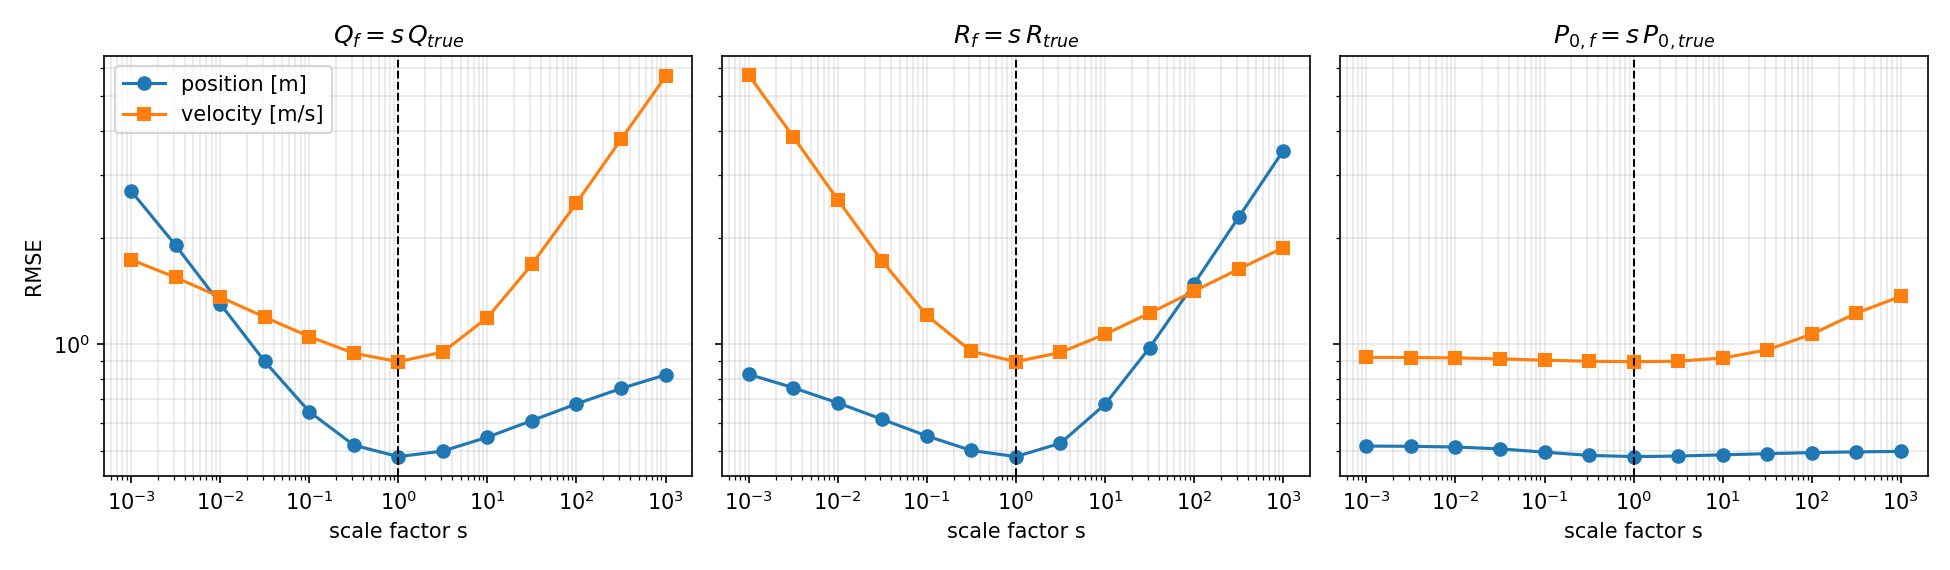
\includegraphics[width=0.7\linewidth]{linear_kf/figures/rmse_vs_s.png}
\caption{Linear KF: RMSE versus the scale factor. Source: \texttt{experiments/linear\_kf/figures/rmse\_vs\_s.png}.}
\end{figure}
\begin{figure}[htbp]\centering
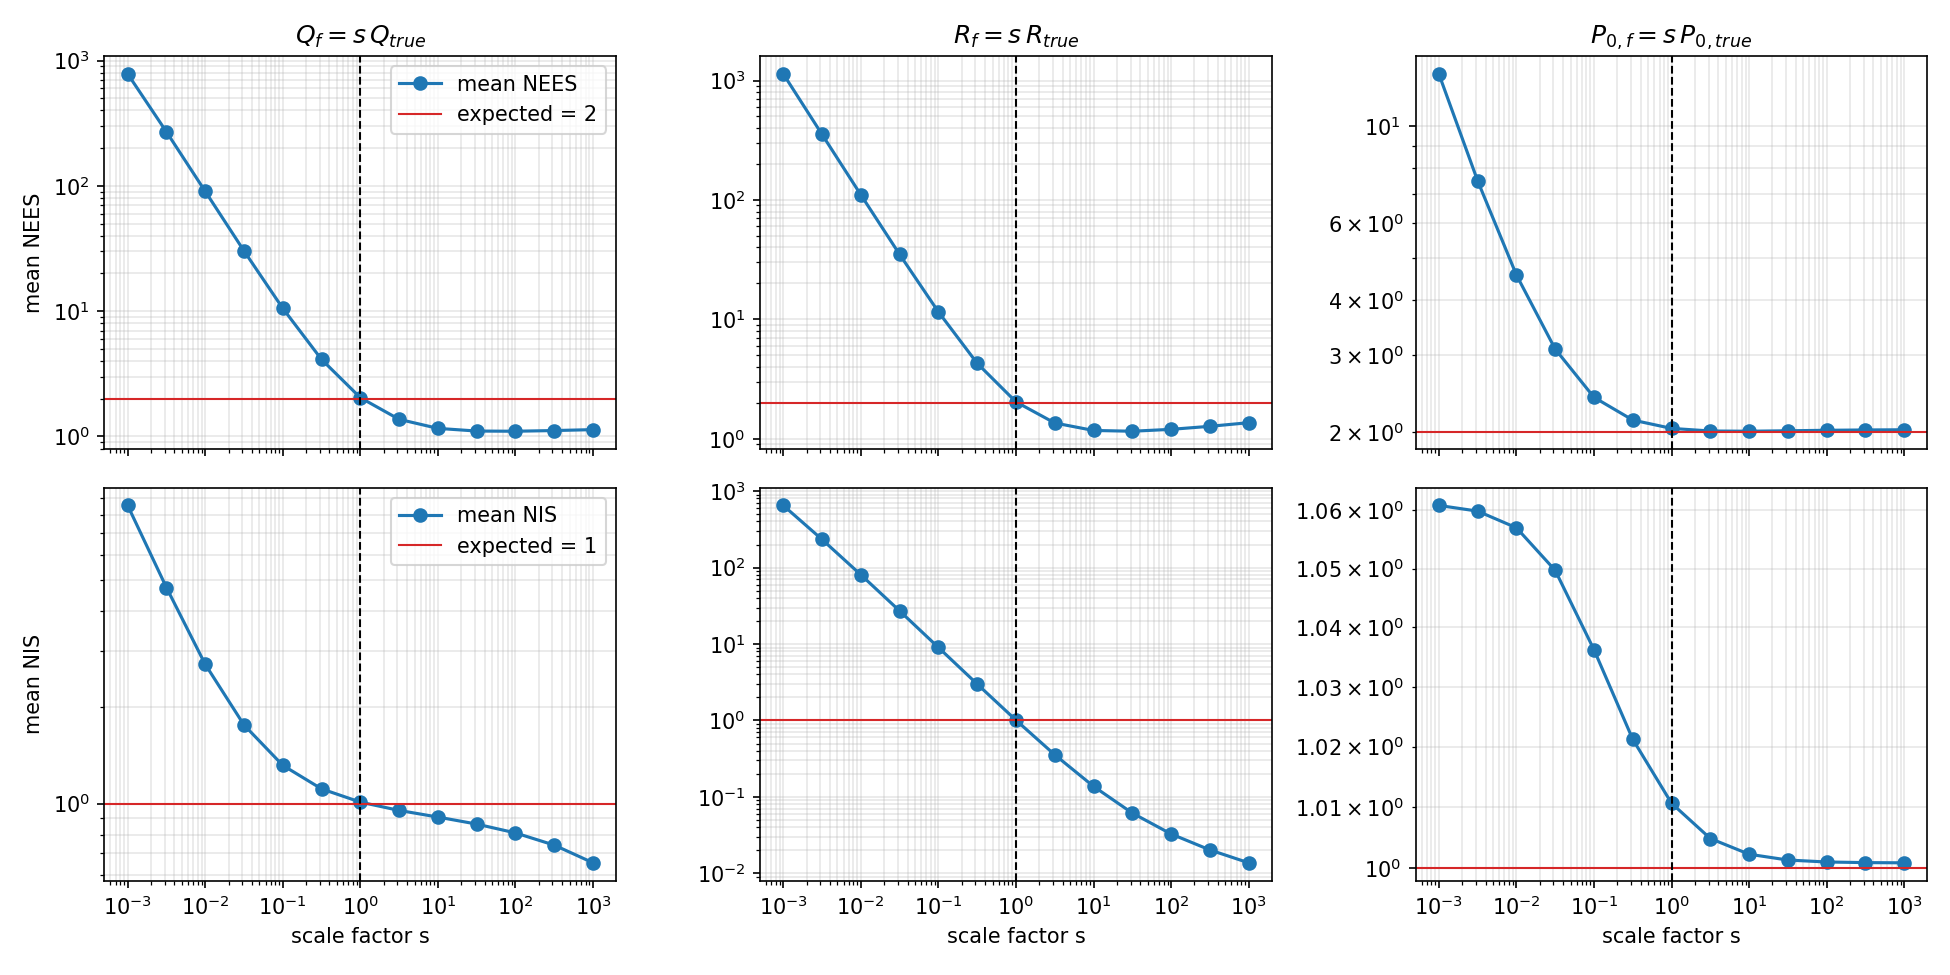
\includegraphics[width=0.7\linewidth]{linear_kf/figures/nees_nis_vs_s.png}
\caption{Linear KF: NEES and NIS versus the scale factor. Source: \texttt{experiments/linear\_kf/figures/nees\_nis\_vs\_s.png}.}
\end{figure}
\begin{figure}[htbp]\centering
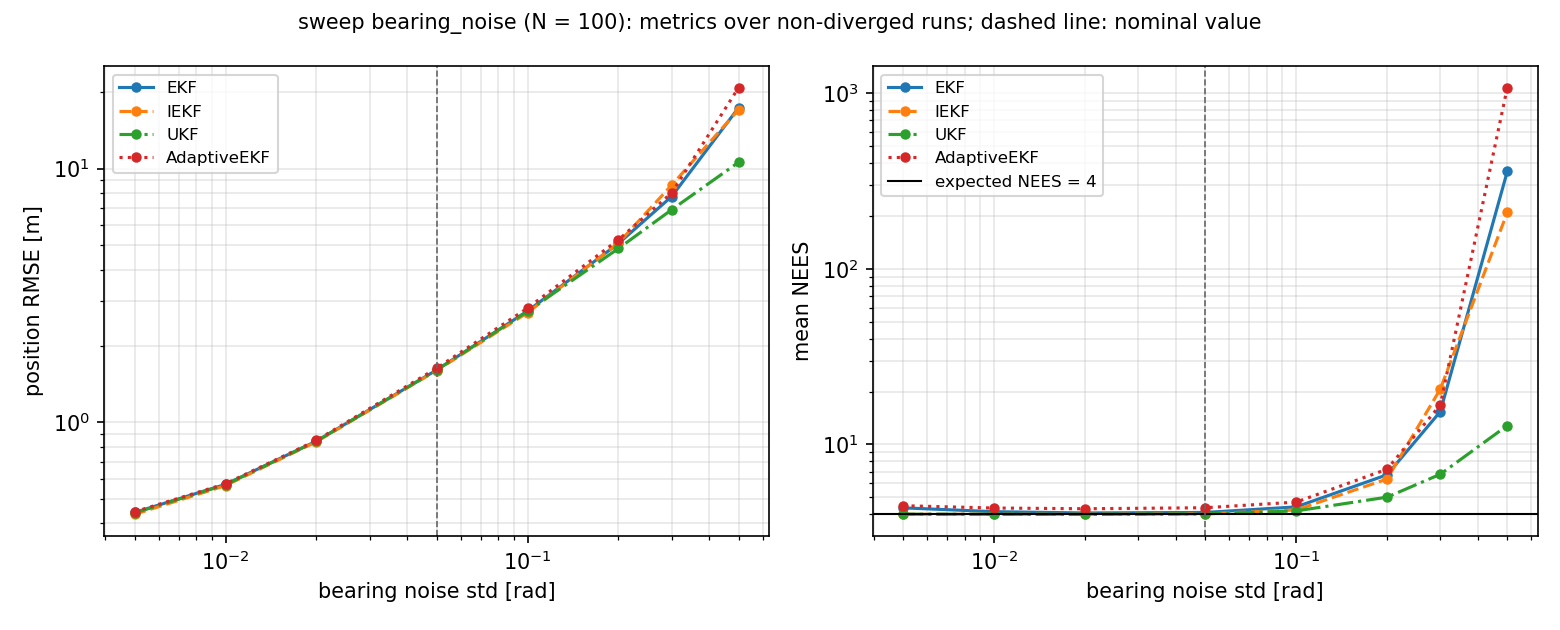
\includegraphics[width=0.75\linewidth]{filter_family/figures/sweep_bearing_noise.png}
\caption{Filter family: RMSE and NEES versus bearing noise. Source: \texttt{experiments/filter\_family/figures/sweep\_bearing\_noise.png}.}
\end{figure}
\begin{figure}[htbp]\centering
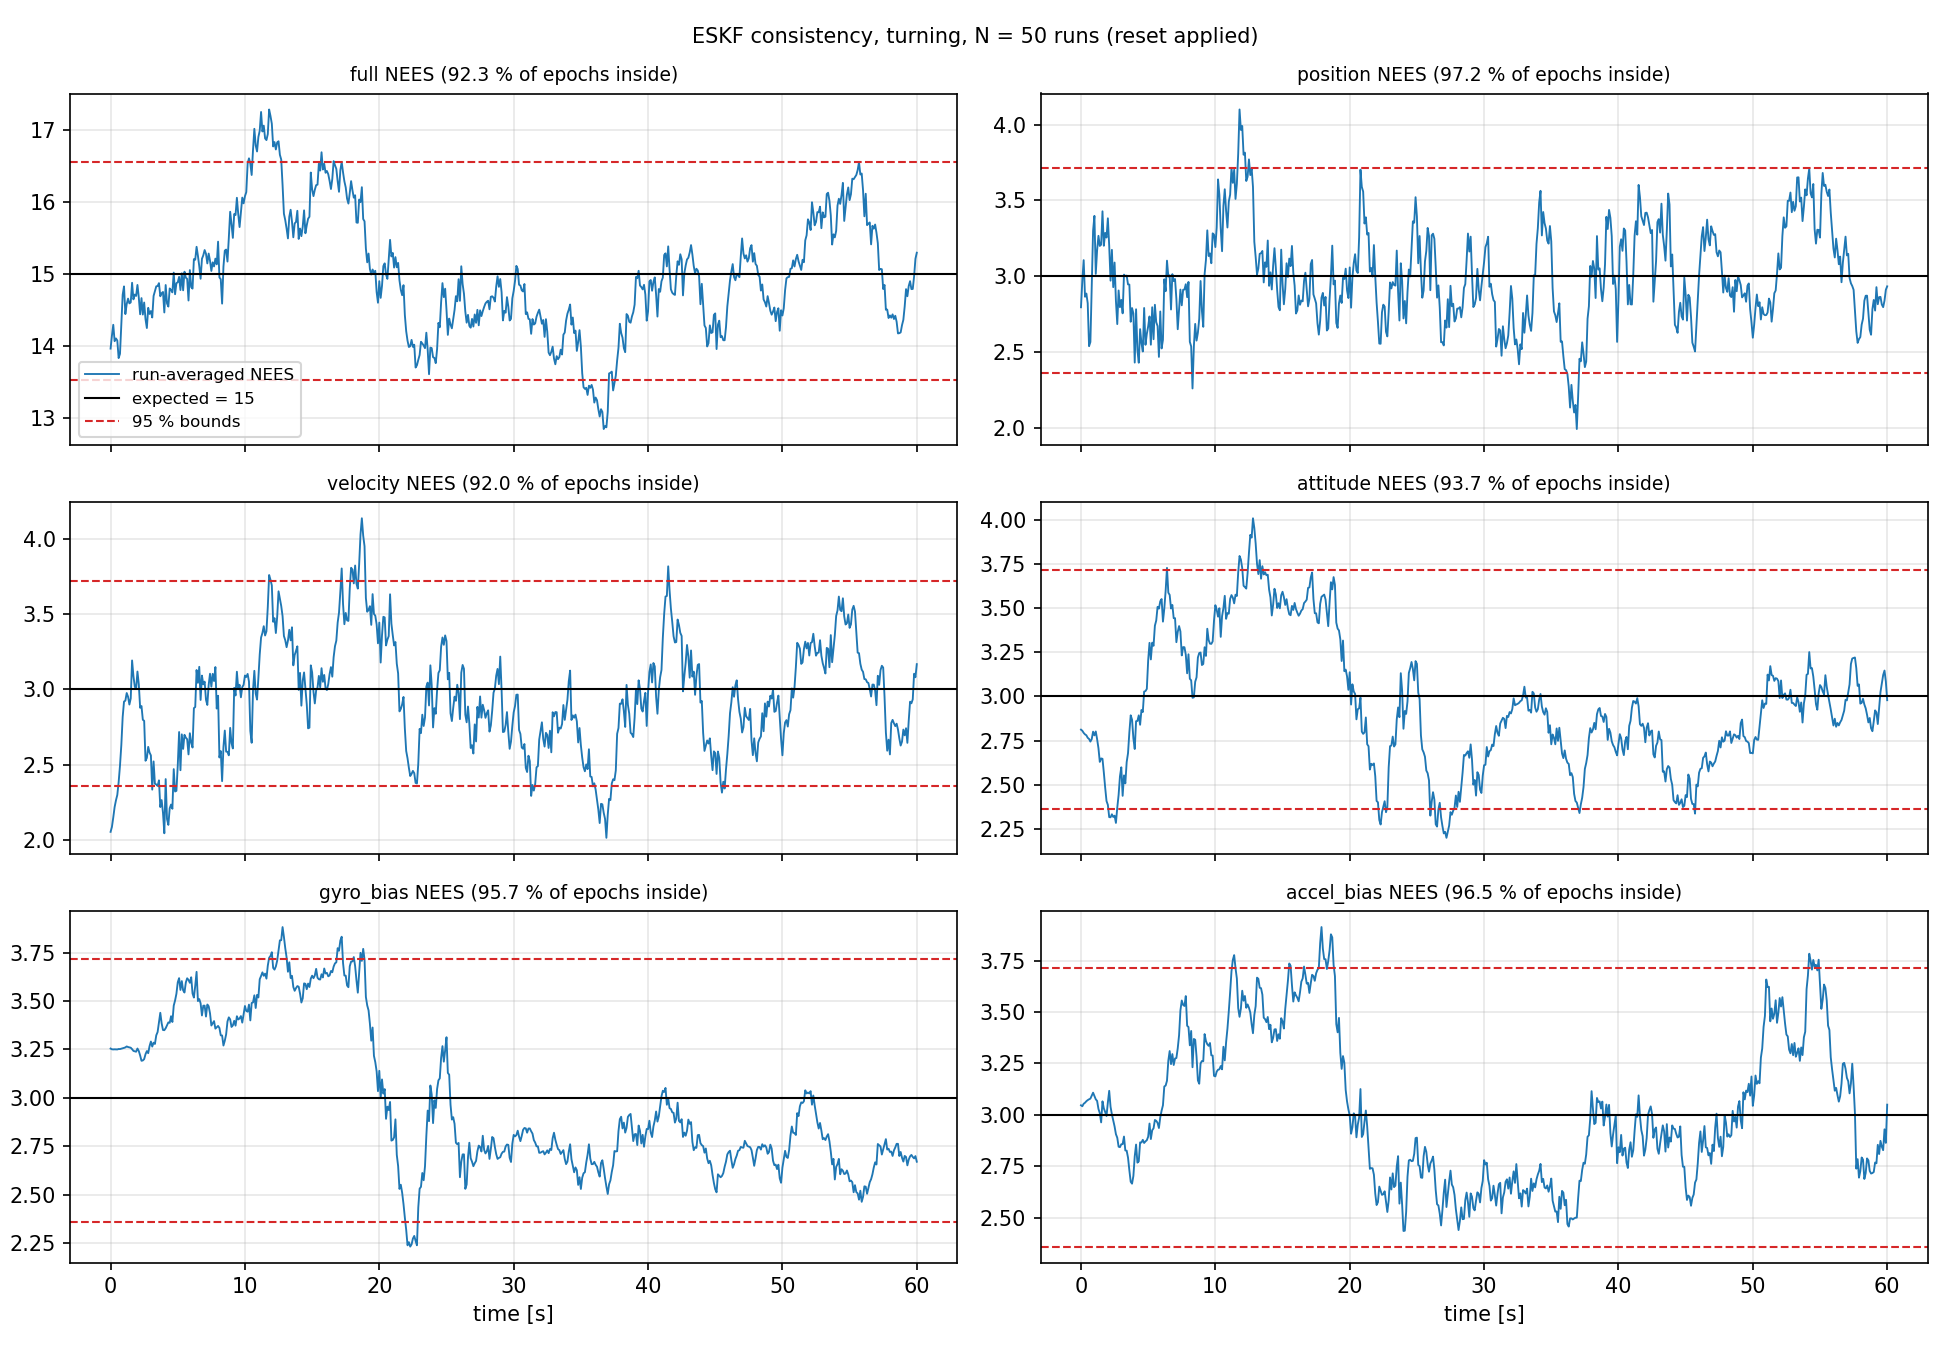
\includegraphics[width=0.8\linewidth]{eskf_sensitivity/figures/consistency_turning.png}
\caption{ESKF, \texttt{turning}: run-averaged NEES with chi-square bounds. Source: \texttt{experiments/eskf\_sensitivity/figures/consistency\_turning.png}.}
\end{figure}
\begin{figure}[htbp]\centering
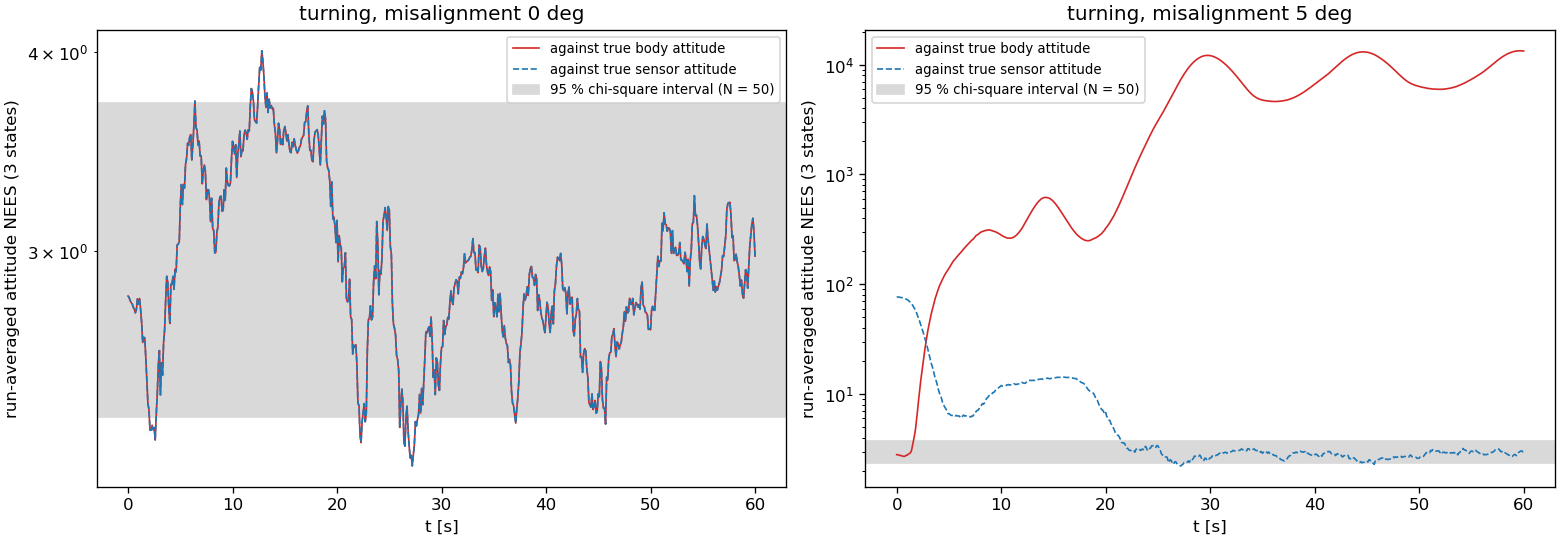
\includegraphics[width=0.8\linewidth]{eskf_sensitivity/figures/attitude_reference.png}
\caption{Attitude NEES against body and sensor attitude. Source: \texttt{experiments/eskf\_sensitivity/figures/attitude\_reference.png}.}
\end{figure}
\begin{figure}[htbp]\centering
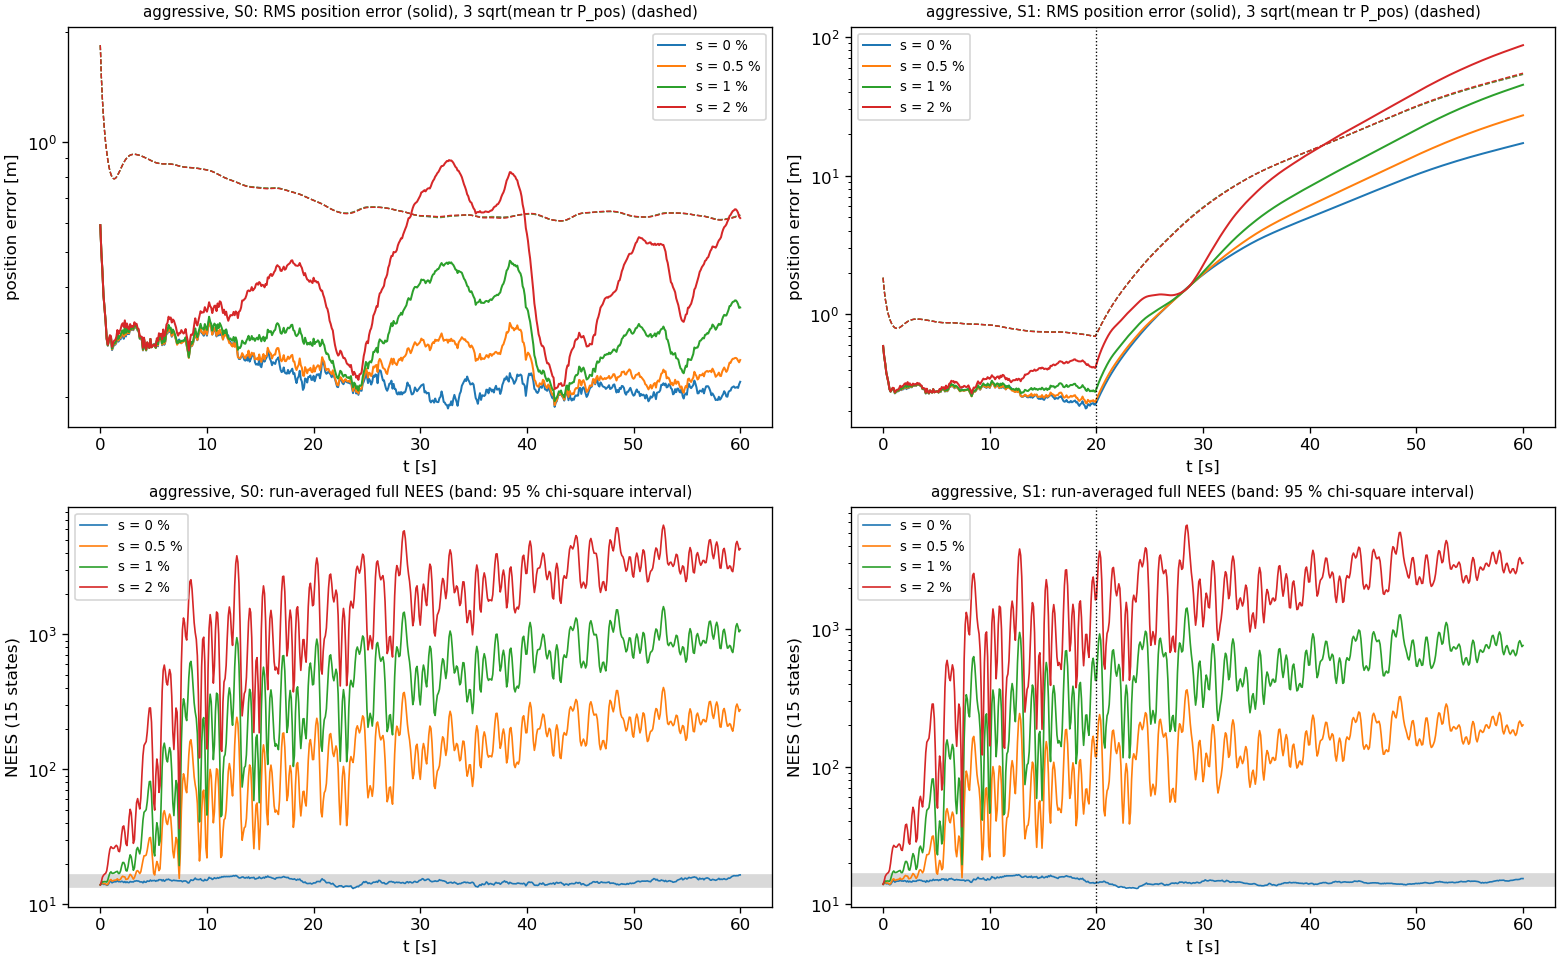
\includegraphics[width=0.85\linewidth]{eskf_sensitivity/figures/scale_factor_aggressive.png}
\caption{Scale factor, \texttt{aggressive}: position error with $3\sigma$ and full NEES for S0 and S1.
Source: \texttt{experiments/eskf\_sensitivity/figures/scale\_factor\_aggressive.png}.}\label{fig:sfagg}
\end{figure}
\begin{figure}[htbp]\centering
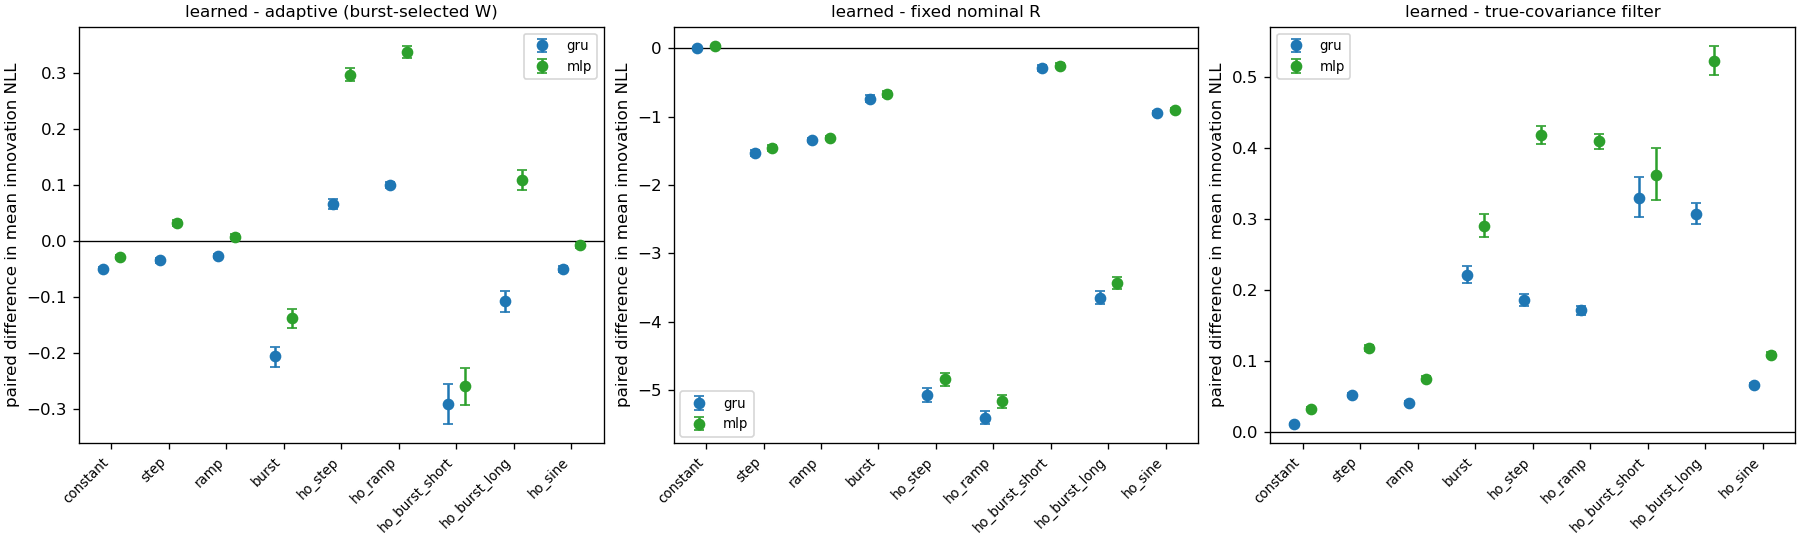
\includegraphics[width=0.85\linewidth]{neural_r/figures/eval_nll_differences.png}
\caption{Paired NLL differences of GRU and MLP against three baselines. Source: \texttt{experiments/neural\_r/figures/eval\_nll\_differences.png}.}
\end{figure}
\begin{figure}[htbp]\centering
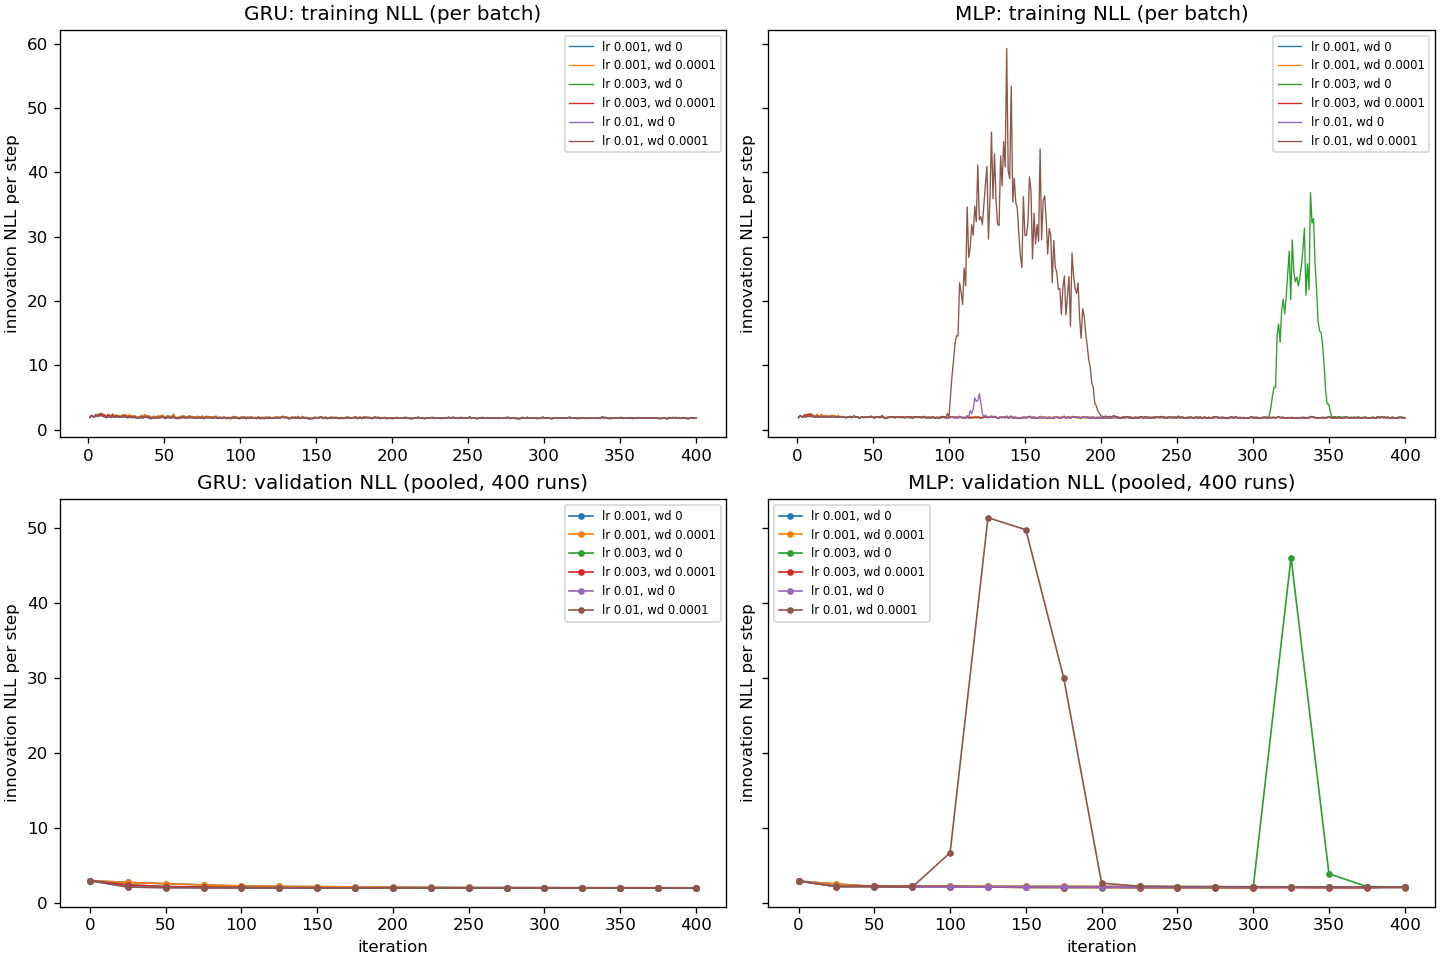
\includegraphics[width=0.8\linewidth]{neural_r/figures/training_curves.png}
\caption{Training and validation NLL of the twelve configurations. Source: \texttt{experiments/neural\_r/figures/training\_curves.png}.}
\end{figure}
\begin{figure}[htbp]\centering
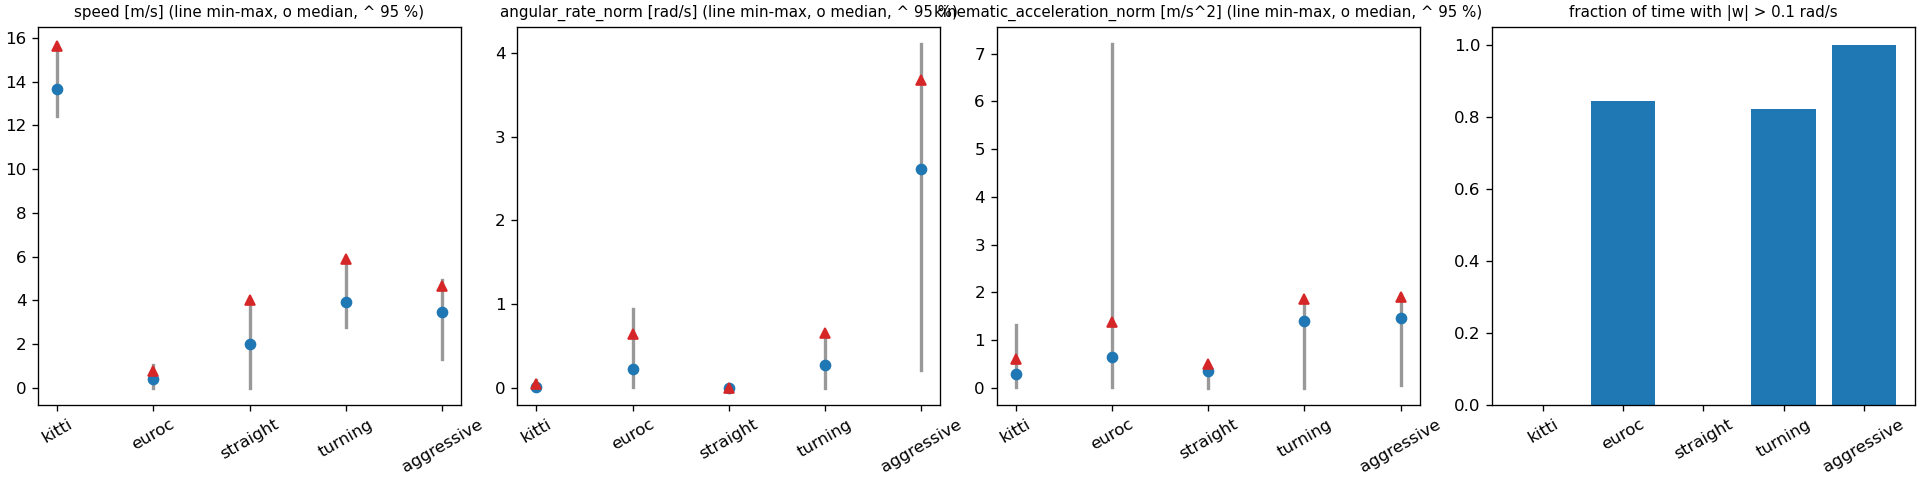
\includegraphics[width=\linewidth]{dataset_char/figures/motion_comparison.png}
\caption{Speed, angular rate, acceleration and turning fraction of the real sequences and synthetic
profiles. Source: \texttt{analysis/dataset\_char/figures/motion\_comparison.png}.}\label{fig:motion}
\end{figure}

%==================================================================================================
\section{Long tables}\label{app:tables}
%==================================================================================================
\subsection*{Linear KF}
\begin{table}[htbp]
\centering
\small
\caption{Linear KF, N = 200 runs, T = 200: one filter quantity scaled, 95\,\% bootstrap intervals over runs. Expected NEES 2, NIS 1. Source: \texttt{experiments/linear\_kf/results/closure\_summary.csv}.}\label{tab:lin_closure}
\resizebox{\linewidth}{!}{%
\begin{tabular}{lllll}
\toprule
Setting & Position RMSE [m] & Velocity RMSE [m/s] & Mean NEES & Mean NIS \\
\midrule
nominal & 0.482 [0.474, 0.490] & 0.893 [0.879, 0.907] & 2.04 [1.99, 2.10] & 1.01 [0.998, 1.02] \\
Q x 0.001 & 2.70 [2.52, 2.88] & 1.73 [1.65, 1.81] & 783 [710, 859] & 8.55 [7.56, 9.61] \\
Q x 1000 & 0.820 [0.814, 0.826] & 5.69 [5.65, 5.73] & 1.13 [1.12, 1.15] & 0.653 [0.643, 0.663] \\
R x 0.001 & 0.823 [0.817, 0.828] & 5.74 [5.70, 5.78] & 1136 [1121, 1153] & 649 [639, 659] \\
R x 1000 & 3.51 [3.31, 3.71] & 1.87 [1.79, 1.95] & 1.37 [1.27, 1.47] & 0.0138 [0.0124, 0.0152] \\
P0 x 0.001 & 0.516 [0.506, 0.527] & 0.919 [0.903, 0.935] & 13.1 [11.1, 15.4] & 1.06 [1.05, 1.08] \\
P0 x 1000 & 0.499 [0.491, 0.507] & 1.37 [1.31, 1.42] & 2.02 [1.97, 2.08] & 1.00 [0.988, 1.01] \\
\bottomrule
\end{tabular}}
\end{table}

\begin{table}[htbp]
\centering
\small
\caption{Common-scale identity on data: configurations that differ by a common factor of all filter covariances give identical RMSE, and NEES and NIS scaled by the inverse factor (T = 200, all steps). The gain-convergence step uses a 1\,\% threshold. Source: \path{experiments/linear_kf/results/open_point.csv}.}\label{tab:lin_scale}
\resizebox{\linewidth}{!}{%
\begin{tabular}{llllllll}
\toprule
Configuration & $Q$ scale & $R$ scale & $P_0$ scale & Pos. RMSE & NEES & NIS & Gain conv. step \\
\midrule
truth & 1.00 & 1.00 & 1.00 & 0.4823 & 2.040 & 1.011 & 22 \\
Q x 0.001 & 0.00100 & 1.00 & 1.00 & 2.704 & 783.4 & 8.554 & 129 \\
R x 1000 & 1.00 & 1000 & 1.00 & 3.512 & 1.365 & 0.01377 & 140 \\
R x 1000, P0 x 1000 & 1.00 & 1000 & 1000 & 2.704 & 0.7834 & 0.008554 & 129 \\
Q x 1000 & 1000 & 1.00 & 1.00 & 0.8199 & 1.134 & 0.6529 & 4 \\
R x 0.001 & 1.00 & 0.00100 & 1.00 & 0.8227 & 1136 & 648.6 & 5 \\
R x 0.001, P0 x 0.001 & 1.00 & 0.00100 & 0.00100 & 0.8199 & 1134 & 652.9 & 4 \\
\bottomrule
\end{tabular}}
\end{table}

\begin{table}[htbp]
\centering
\small
\caption{Linear KF: paired differences (A minus B) on the same runs. Source: \texttt{experiments/linear\_kf/results/closure\_paired.csv}.}\label{tab:lin_paired}
\resizebox{\linewidth}{!}{%
\begin{tabular}{lllll}
\toprule
A & B & Metric & Difference [95\,\% CI] & Supported \\
\midrule
Q x 1000 & R x 0.001 & pos\_rmse & -0.00282 [-0.00333, -0.00233] & True \\
Q x 0.001 & R x 1000 & pos\_rmse & -0.808 [-0.933, -0.688] & True \\
P0 x 0.001 & nominal & pos\_rmse & 0.0342 [0.0268, 0.0421] & True \\
P0 x 1000 & nominal & pos\_rmse & 0.0166 [0.0141, 0.0191] & True \\
\bottomrule
\end{tabular}}
\end{table}

\subsection*{Filter family}
\begin{table}[htbp]
\centering
\small
\caption{Nominal range-bearing comparison (N = 100, 60 steps) with the wall-clock time per predict and update step in pure Python and NumPy (relative comparison only). Source: \path{experiments/filter_family/results/nominal_comparison.csv}.}\label{tab:ff_runtime}
\resizebox{\linewidth}{!}{%
\begin{tabular}{llllll}
\toprule
Filter & Pos. RMSE [m] & NEES & NIS & Time per step [$\mu$s] & Mean IEKF iterations \\
\midrule
EKF & 1.61 & 4.10 & 2.04 & 18.5 & -- \\
IEKF & 1.60 & 4.03 & 2.03 & 125 & 6.79 \\
UKF & 1.61 & 4.03 & 2.02 & 35.3 & -- \\
AdaptiveEKF & 1.63 & 4.36 & 2.23 & 31.7 & -- \\
\bottomrule
\end{tabular}}
\end{table}

{\scriptsize
\begin{longtable}{llllll}
\caption{Range-bearing benchmark, N = 100 runs, 60 steps: divergence count and metrics over non-diverged runs with 95\,\% intervals. Expected NEES 4, NIS 2. Source: \path{experiments/filter_family/results/closure_summary.csv}.}\label{tab:ff_closure}\\
\toprule
Setting & Filter & Div. & Position RMSE [m] & Mean NEES & Mean NIS \\
\midrule
\endfirsthead
\toprule
Setting & Filter & Div. & Position RMSE [m] & Mean NEES & Mean NIS \\
\midrule
\endhead
nominal & EKF & 0 & 1.61 [1.50, 1.72] & 4.10 [3.93, 4.28] & 2.04 [1.99, 2.09] \\
nominal & IEKF & 0 & 1.60 [1.50, 1.71] & 4.03 [3.87, 4.20] & 2.03 [1.99, 2.08] \\
nominal & UKF & 0 & 1.61 [1.50, 1.72] & 4.03 [3.86, 4.20] & 2.02 [1.97, 2.07] \\
nominal & AdaptiveEKF & 0 & 1.63 [1.52, 1.75] & 4.36 [4.17, 4.56] & 2.23 [2.20, 2.26] \\
initial std 40 m & EKF & 0 & 6.90 [5.92, 7.83] & 179 [112, 258] & 8.14 [6.07, 10.4] \\
initial std 40 m & IEKF & 0 & 2.04 [1.87, 2.21] & 4.10 [3.93, 4.29] & 2.04 [1.99, 2.09] \\
initial std 40 m & UKF & 0 & 5.38 [4.49, 6.40] & 4.21 [3.99, 4.44] & 2.04 [1.95, 2.16] \\
initial std 40 m & AdaptiveEKF & 0 & 7.65 [6.44, 8.84] & 181 [113, 261] & 7.95 [5.93, 10.2] \\
bearing noise 0.5 rad & EKF & 0 & 17.4 [12.8, 22.8] & 359 [77.2, 883] & 2.16 [2.08, 2.25] \\
bearing noise 0.5 rad & IEKF & 0 & 17.1 [14.8, 19.4] & 209 [138, 296] & 2.31 [2.22, 2.41] \\
bearing noise 0.5 rad & UKF & 0 & 10.6 [9.08, 12.2] & 12.8 [8.57, 18.4] & 1.47 [1.42, 1.52] \\
bearing noise 0.5 rad & AdaptiveEKF & 0 & 20.9 [13.4, 29.2] & 1078 [84.2, 2796] & 2.13 [2.09, 2.17] \\
R x 100 & EKF & 0 & 5.56 [4.90, 6.25] & 2.41 [2.20, 2.63] & 0.119 [0.110, 0.129] \\
R x 100 & IEKF & 0 & 5.44 [4.82, 6.06] & 2.36 [2.17, 2.57] & 0.119 [0.110, 0.129] \\
R x 100 & UKF & 0 & 5.50 [4.86, 6.15] & 2.40 [2.22, 2.61] & 0.118 [0.108, 0.128] \\
R x 100 & AdaptiveEKF & 0 & 3.80 [3.33, 4.26] & 3.25 [3.08, 3.43] & 1.11 [1.08, 1.14] \\
Q x 0.01 & EKF & 0 & 3.79 [3.28, 4.30] & 151 [138, 164] & 6.21 [5.77, 6.69] \\
Q x 0.01 & IEKF & 0 & 3.80 [3.28, 4.31] & 150 [137, 164] & 6.21 [5.76, 6.69] \\
Q x 0.01 & UKF & 0 & 3.75 [3.25, 4.25] & 149 [136, 162] & 6.15 [5.71, 6.62] \\
Q x 0.01 & AdaptiveEKF & 1 & 7.26 [6.19, 8.30] & 180 [162, 201] & 3.67 [3.55, 3.78] \\
P0 x 100 & EKF & 0 & 1.66 [1.56, 1.77] & 4.11 [3.93, 4.29] & 1.98 [1.93, 2.02] \\
P0 x 100 & IEKF & 0 & 1.65 [1.55, 1.76] & 4.00 [3.84, 4.18] & 1.97 [1.92, 2.02] \\
P0 x 100 & UKF & 0 & 3.47 [3.33, 3.60] & 3.64 [3.49, 3.80] & 1.78 [1.73, 1.82] \\
P0 x 100 & AdaptiveEKF & 0 & 1.69 [1.58, 1.80] & 4.37 [4.18, 4.57] & 2.17 [2.14, 2.20] \\
\bottomrule
\end{longtable}
}

{\scriptsize
\begin{longtable}{llll}
\caption{Range-bearing benchmark, same settings as Table~\ref{tab:ff_closure}: mean NEES (expected 4) and mean NIS (expected 2) with 95\,\% intervals. Source: \path{experiments/filter_family/results/closure_summary.csv}.}\label{tab:ff_closure_cons}\\
\toprule
Setting & Filter & Mean NEES & Mean NIS \\
\midrule
\endfirsthead
\toprule
Setting & Filter & Mean NEES & Mean NIS \\
\midrule
\endhead
nominal & EKF & 4.10 [3.93, 4.28] & 2.04 [1.99, 2.09] \\
nominal & IEKF & 4.03 [3.87, 4.20] & 2.03 [1.99, 2.08] \\
nominal & UKF & 4.03 [3.86, 4.20] & 2.02 [1.97, 2.07] \\
nominal & AdaptiveEKF & 4.36 [4.17, 4.56] & 2.23 [2.20, 2.26] \\
initial std 40 m & EKF & 179 [112, 258] & 8.14 [6.07, 10.4] \\
initial std 40 m & IEKF & 4.10 [3.93, 4.29] & 2.04 [1.99, 2.09] \\
initial std 40 m & UKF & 4.21 [3.99, 4.44] & 2.04 [1.95, 2.16] \\
initial std 40 m & AdaptiveEKF & 181 [113, 261] & 7.95 [5.93, 10.2] \\
bearing noise 0.5 rad & EKF & 359 [77.2, 883] & 2.16 [2.08, 2.25] \\
bearing noise 0.5 rad & IEKF & 209 [138, 296] & 2.31 [2.22, 2.41] \\
bearing noise 0.5 rad & UKF & 12.8 [8.57, 18.4] & 1.47 [1.42, 1.52] \\
bearing noise 0.5 rad & AdaptiveEKF & 1078 [84.2, 2796] & 2.13 [2.09, 2.17] \\
R x 100 & EKF & 2.41 [2.20, 2.63] & 0.119 [0.110, 0.129] \\
R x 100 & IEKF & 2.36 [2.17, 2.57] & 0.119 [0.110, 0.129] \\
R x 100 & UKF & 2.40 [2.22, 2.61] & 0.118 [0.108, 0.128] \\
R x 100 & AdaptiveEKF & 3.25 [3.08, 3.43] & 1.11 [1.08, 1.14] \\
Q x 0.01 & EKF & 151 [138, 164] & 6.21 [5.77, 6.69] \\
Q x 0.01 & IEKF & 150 [137, 164] & 6.21 [5.76, 6.69] \\
Q x 0.01 & UKF & 149 [136, 162] & 6.15 [5.71, 6.62] \\
Q x 0.01 & AdaptiveEKF & 180 [162, 201] & 3.67 [3.55, 3.78] \\
P0 x 100 & EKF & 4.11 [3.93, 4.29] & 1.98 [1.93, 2.02] \\
P0 x 100 & IEKF & 4.00 [3.84, 4.18] & 1.97 [1.92, 2.02] \\
P0 x 100 & UKF & 3.64 [3.49, 3.80] & 1.78 [1.73, 1.82] \\
P0 x 100 & AdaptiveEKF & 4.37 [4.18, 4.57] & 2.17 [2.14, 2.20] \\
\bottomrule
\end{longtable}
}

{\small
\begin{longtable}{llllll}
\caption{Filter family: the 59 supported paired differences (A minus B) out of 72 computed; all others have intervals containing zero. Source: \texttt{experiments/filter\_family/results/closure\_paired.csv}.}\label{tab:ff_paired}\\
\toprule
Setting & A & B & Metric & Difference [95\,\% CI] & Runs \\
\midrule
\endfirsthead
\toprule
Setting & A & B & Metric & Difference [95\,\% CI] & Runs \\
\midrule
\endhead
nominal & EKF & IEKF & mean\_nees & 0.0741 [0.0530, 0.0962] & 100 \\
nominal & EKF & UKF & mean\_nees & 0.0732 [0.0551, 0.0918] & 100 \\
nominal & EKF & AdaptiveEKF & pos\_rmse & -0.0264 [-0.0479, -0.00526] & 100 \\
nominal & EKF & AdaptiveEKF & mean\_nees & -0.261 [-0.331, -0.193] & 100 \\
nominal & IEKF & AdaptiveEKF & pos\_rmse & -0.0337 [-0.0566, -0.0119] & 100 \\
nominal & IEKF & AdaptiveEKF & mean\_nees & -0.335 [-0.409, -0.266] & 100 \\
nominal & UKF & AdaptiveEKF & pos\_rmse & -0.0265 [-0.0479, -0.00539] & 100 \\
nominal & UKF & AdaptiveEKF & mean\_nees & -0.334 [-0.404, -0.266] & 100 \\
initial std 40 m & EKF & IEKF & pos\_rmse & 4.86 [3.89, 5.80] & 100 \\
initial std 40 m & EKF & IEKF & mean\_nees & 175 [108, 254] & 100 \\
initial std 40 m & EKF & UKF & pos\_rmse & 1.52 [0.683, 2.36] & 100 \\
initial std 40 m & EKF & UKF & mean\_nees & 175 [108, 254] & 100 \\
initial std 40 m & EKF & AdaptiveEKF & pos\_rmse & -0.748 [-1.23, -0.338] & 100 \\
initial std 40 m & EKF & AdaptiveEKF & mean\_nees & -1.51 [-2.98, -0.517] & 100 \\
initial std 40 m & IEKF & UKF & pos\_rmse & -3.34 [-4.36, -2.49] & 100 \\
initial std 40 m & IEKF & AdaptiveEKF & pos\_rmse & -5.61 [-6.79, -4.41] & 100 \\
initial std 40 m & IEKF & AdaptiveEKF & mean\_nees & -177 [-256, -109] & 100 \\
initial std 40 m & UKF & AdaptiveEKF & pos\_rmse & -2.27 [-3.35, -1.21] & 100 \\
initial std 40 m & UKF & AdaptiveEKF & mean\_nees & -177 [-256, -109] & 100 \\
bearing noise 0.5 rad & EKF & UKF & pos\_rmse & 6.80 [2.88, 12.1] & 100 \\
bearing noise 0.5 rad & EKF & UKF & mean\_nees & 346 [66.0, 869] & 100 \\
bearing noise 0.5 rad & EKF & AdaptiveEKF & pos\_rmse & -3.47 [-6.76, -0.0776] & 100 \\
bearing noise 0.5 rad & EKF & AdaptiveEKF & mean\_nees & -719 [-1916, -3.25] & 100 \\
bearing noise 0.5 rad & IEKF & UKF & pos\_rmse & 6.48 [4.57, 8.24] & 100 \\
bearing noise 0.5 rad & IEKF & UKF & mean\_nees & 197 [127, 280] & 100 \\
bearing noise 0.5 rad & UKF & AdaptiveEKF & pos\_rmse & -10.3 [-18.6, -3.27] & 100 \\
bearing noise 0.5 rad & UKF & AdaptiveEKF & mean\_nees & -1065 [-2782, -72.6] & 100 \\
R x 100 & EKF & IEKF & pos\_rmse & 0.123 [0.0513, 0.215] & 100 \\
R x 100 & EKF & IEKF & mean\_nees & 0.0445 [0.0271, 0.0654] & 100 \\
R x 100 & EKF & AdaptiveEKF & pos\_rmse & 1.76 [1.36, 2.23] & 100 \\
R x 100 & EKF & AdaptiveEKF & mean\_nees & -0.845 [-1.01, -0.683] & 100 \\
R x 100 & IEKF & UKF & pos\_rmse & -0.0602 [-0.115, -0.00499] & 100 \\
R x 100 & IEKF & UKF & mean\_nees & -0.0434 [-0.0681, -0.0183] & 100 \\
R x 100 & IEKF & AdaptiveEKF & pos\_rmse & 1.64 [1.27, 2.05] & 100 \\
R x 100 & IEKF & AdaptiveEKF & mean\_nees & -0.890 [-1.05, -0.732] & 100 \\
R x 100 & UKF & AdaptiveEKF & pos\_rmse & 1.70 [1.30, 2.14] & 100 \\
R x 100 & UKF & AdaptiveEKF & mean\_nees & -0.846 [-1.00, -0.689] & 100 \\
Q x 0.01 & EKF & IEKF & mean\_nees & 0.697 [0.359, 1.06] & 99 \\
Q x 0.01 & EKF & UKF & pos\_rmse & 0.0429 [0.0206, 0.0664] & 99 \\
Q x 0.01 & EKF & UKF & mean\_nees & 2.06 [1.56, 2.63] & 99 \\
Q x 0.01 & EKF & AdaptiveEKF & pos\_rmse & -3.45 [-4.16, -2.72] & 99 \\
Q x 0.01 & EKF & AdaptiveEKF & mean\_nees & -30.2 [-39.2, -22.3] & 99 \\
Q x 0.01 & IEKF & UKF & pos\_rmse & 0.0462 [0.0218, 0.0695] & 99 \\
Q x 0.01 & IEKF & UKF & mean\_nees & 1.36 [0.936, 1.84] & 99 \\
Q x 0.01 & IEKF & AdaptiveEKF & pos\_rmse & -3.45 [-4.16, -2.72] & 99 \\
Q x 0.01 & IEKF & AdaptiveEKF & mean\_nees & -30.9 [-39.9, -23.0] & 99 \\
Q x 0.01 & UKF & AdaptiveEKF & pos\_rmse & -3.50 [-4.21, -2.76] & 99 \\
Q x 0.01 & UKF & AdaptiveEKF & mean\_nees & -32.3 [-41.5, -24.3] & 99 \\
P0 x 100 & EKF & IEKF & mean\_nees & 0.107 [0.0744, 0.142] & 100 \\
P0 x 100 & EKF & UKF & pos\_rmse & -1.80 [-1.94, -1.68] & 100 \\
P0 x 100 & EKF & UKF & mean\_nees & 0.468 [0.398, 0.541] & 100 \\
P0 x 100 & EKF & AdaptiveEKF & pos\_rmse & -0.0247 [-0.0452, -0.00470] & 100 \\
P0 x 100 & EKF & AdaptiveEKF & mean\_nees & -0.260 [-0.330, -0.194] & 100 \\
P0 x 100 & IEKF & UKF & pos\_rmse & -1.81 [-1.95, -1.69] & 100 \\
P0 x 100 & IEKF & UKF & mean\_nees & 0.362 [0.304, 0.422] & 100 \\
P0 x 100 & IEKF & AdaptiveEKF & pos\_rmse & -0.0345 [-0.0567, -0.0135] & 100 \\
P0 x 100 & IEKF & AdaptiveEKF & mean\_nees & -0.367 [-0.445, -0.296] & 100 \\
P0 x 100 & UKF & AdaptiveEKF & pos\_rmse & 1.78 [1.65, 1.92] & 100 \\
P0 x 100 & UKF & AdaptiveEKF & mean\_nees & -0.728 [-0.824, -0.635] & 100 \\
\bottomrule
\end{longtable}
}

\subsection*{ESKF}
{\scriptsize
\begin{longtable}{llll}
\caption{ESKF sensitivity, profile \texttt{turning} unless varied, N = 30 runs: nominal setting and the end points of every sweep, accuracy with 95\,\% intervals (consistency in Table~\ref{tab:es_closure_cons}). Source: \texttt{experiments/eskf\_sensitivity/results/closure\_summary.csv}.}\label{tab:es_closure}\\
\toprule
Setting & Failed & Pos. RMSE [m] & Att. RMSE [deg] \\
\midrule
\endfirsthead
\toprule
Setting & Failed & Pos. RMSE [m] & Att. RMSE [deg] \\
\midrule
\endhead
nominal & 0 & 0.247 [0.242, 0.252] & 0.919 [0.834, 1.01] \\
q\_imu 0.01 & 0 & 0.248 [0.243, 0.254] & 0.926 [0.841, 1.01] \\
q\_imu 100 & 0 & 0.264 [0.260, 0.269] & 1.04 [0.934, 1.14] \\
q\_bias 0.01 & 0 & 0.301 [0.285, 0.317] & 0.937 [0.858, 1.02] \\
q\_bias 100 & 0 & 0.284 [0.280, 0.289] & 1.07 [0.960, 1.17] \\
r 0.01 & 0 & 0.315 [0.311, 0.319] & 2.49 [2.35, 2.64] \\
r 100 & 0 & 0.735 [0.693, 0.776] & 1.63 [1.37, 1.91] \\
p0 0.01 & 0 & 0.538 [0.504, 0.572] & 1.86 [1.51, 2.21] \\
p0 100 & 0 & 0.279 [0.275, 0.284] & 2.53 [2.34, 2.74] \\
bias\_estimation 0 (enabled) & 0 & 0.224 [0.219, 0.229] & 0.383 [0.346, 0.416] \\
bias\_estimation 0 (disabled) & 0 & 0.878 [0.713, 1.03] & 0.415 [0.377, 0.451] \\
bias\_estimation 10 (enabled) & 0 & 0.271 [0.265, 0.278] & 3.01 [2.66, 3.36] \\
bias\_estimation 10 (disabled) & 0 & 24.8 [20.2, 29.2] & 32.5 [25.9, 39.0] \\
dropout 0 & 0 & 0.247 [0.242, 0.252] & 0.919 [0.834, 1.01] \\
dropout 40 & 0 & 26.8 [23.4, 30.1] & 3.14 [2.59, 3.67] \\
outliers 0 (gate off) & 0 & 0.247 [0.242, 0.252] & 0.919 [0.834, 1.01] \\
outliers 0 (gate on) & 0 & 0.248 [0.243, 0.254] & 0.923 [0.837, 1.01] \\
outliers 0.2 (gate off) & 0 & 0.646 [0.631, 0.660] & 1.79 [1.62, 1.99] \\
outliers 0.2 (gate on) & 0 & 0.274 [0.268, 0.282] & 0.981 [0.896, 1.07] \\
imu\_spikes 0 & 0 & 0.247 [0.242, 0.252] & 0.919 [0.834, 1.01] \\
imu\_spikes 0.01 & 0 & 0.640 [0.576, 0.711] & 2.98 [2.62, 3.35] \\
profile straight & 0 & 0.239 [0.233, 0.245] & 1.51 [1.33, 1.69] \\
profile aggressive & 0 & 0.237 [0.232, 0.242] & 0.746 [0.676, 0.817] \\
meas\_rate 1 & 0 & 0.652 [0.632, 0.674] & 1.34 [1.17, 1.52] \\
meas\_rate 20 & 0 & 0.188 [0.183, 0.193] & 0.840 [0.783, 0.906] \\
\bottomrule
\end{longtable}
}

{\scriptsize
\begin{longtable}{lll}
\caption{ESKF sensitivity, same settings as Table~\ref{tab:es_closure}: mean position NEES and mean NIS with 95\,\% intervals (expected 3 each). Source: \texttt{experiments/eskf\_sensitivity/results/closure\_summary.csv}.}\label{tab:es_closure_cons}\\
\toprule
Setting & Pos. NEES & NIS \\
\midrule
\endfirsthead
\toprule
Setting & Pos. NEES & NIS \\
\midrule
\endhead
nominal & 3.02 [2.90, 3.14] & 2.97 [2.95, 3.00] \\
q\_imu 0.01 & 3.16 [3.02, 3.31] & 2.98 [2.96, 3.01] \\
q\_imu 100 & 2.78 [2.68, 2.87] & 2.95 [2.92, 2.98] \\
q\_bias 0.01 & 7.98 [6.66, 9.45] & 3.13 [3.08, 3.18] \\
q\_bias 100 & 2.68 [2.60, 2.76] & 2.93 [2.90, 2.96] \\
r 0.01 & 266 [258, 273] & 291 [288, 293] \\
r 100 & 0.640 [0.573, 0.706] & 0.0513 [0.0489, 0.0536] \\
p0 0.01 & 32.0 [27.7, 36.4] & 4.01 [3.88, 4.15] \\
p0 100 & 2.98 [2.86, 3.10] & 2.95 [2.92, 2.98] \\
bias\_estimation 0 (enabled) & 2.97 [2.84, 3.11] & 2.97 [2.94, 3.00] \\
bias\_estimation 0 (disabled) & 177 [113, 251] & 6.01 [4.92, 7.26] \\
bias\_estimation 10 (enabled) & 3.14 [2.96, 3.31] & 2.98 [2.95, 3.01] \\
bias\_estimation 10 (disabled) & $1.17\times10^{5}$ [72089, $1.69\times10^{5}$] & 2528 [1681, 3493] \\
dropout 0 & 3.02 [2.90, 3.14] & 2.97 [2.95, 3.00] \\
dropout 40 & 3.19 [2.82, 3.59] & 2.97 [2.91, 3.02] \\
outliers 0 (gate off) & 3.02 [2.90, 3.14] & 2.97 [2.95, 3.00] \\
outliers 0 (gate on) & 3.04 [2.90, 3.17] & 2.96 [2.93, 2.99] \\
outliers 0.2 (gate off) & 20.6 [19.6, 21.6] & 22.3 [21.7, 22.9] \\
outliers 0.2 (gate on) & 3.01 [2.87, 3.16] & 2.98 [2.95, 3.01] \\
imu\_spikes 0 & 3.02 [2.90, 3.14] & 2.97 [2.95, 3.00] \\
imu\_spikes 0.01 & 23.4 [18.8, 29.1] & 4.47 [4.14, 4.88] \\
profile straight & 3.02 [2.89, 3.17] & 2.98 [2.95, 3.01] \\
profile aggressive & 3.02 [2.87, 3.18] & 2.98 [2.95, 3.00] \\
meas\_rate 1 & 2.92 [2.72, 3.14] & 2.95 [2.86, 3.04] \\
meas\_rate 20 & 3.04 [2.89, 3.22] & 2.98 [2.96, 3.00] \\
\bottomrule
\end{longtable}
}

{\small
\begin{longtable}{llll}
\caption{ESKF: paired differences to the nominal setting (same run indices). Source: \path{experiments/eskf_sensitivity/results/closure_paired.csv}.}\label{tab:es_paired}\\
\toprule
Setting & Metric & Minus nominal [95\,\% CI] & Supported \\
\midrule
\endfirsthead
\toprule
Setting & Metric & Minus nominal [95\,\% CI] & Supported \\
\midrule
\endhead
q\_imu 0.01 & pos\_rmse & 0.00133 [$-5.07\times10^{-8}$, 0.00267] & False \\
q\_imu 0.01 & mean\_nees\_pos & 0.145 [0.0989, 0.191] & True \\
q\_imu 100 & pos\_rmse & 0.0174 [0.0149, 0.0198] & True \\
q\_imu 100 & mean\_nees\_pos & -0.241 [-0.302, -0.182] & True \\
q\_bias 0.01 & pos\_rmse & 0.0539 [0.0395, 0.0690] & True \\
q\_bias 0.01 & mean\_nees\_pos & 4.96 [3.67, 6.42] & True \\
q\_bias 100 & pos\_rmse & 0.0372 [0.0338, 0.0406] & True \\
q\_bias 100 & mean\_nees\_pos & -0.337 [-0.429, -0.250] & True \\
r 0.01 & pos\_rmse & 0.0679 [0.0628, 0.0725] & True \\
r 0.01 & mean\_nees\_pos & 263 [255, 270] & True \\
r 100 & pos\_rmse & 0.488 [0.450, 0.526] & True \\
r 100 & mean\_nees\_pos & -2.38 [-2.49, -2.26] & True \\
p0 0.01 & pos\_rmse & 0.291 [0.258, 0.323] & True \\
p0 0.01 & mean\_nees\_pos & 29.0 [24.7, 33.4] & True \\
p0 100 & pos\_rmse & 0.0326 [0.0283, 0.0368] & True \\
p0 100 & mean\_nees\_pos & -0.0386 [-0.119, 0.0494] & False \\
bias\_estimation 0 (enabled) & pos\_rmse & -0.0229 [-0.0260, -0.0197] & True \\
bias\_estimation 0 (enabled) & mean\_nees\_pos & -0.0466 [-0.113, 0.0211] & False \\
bias\_estimation 0 (disabled) & pos\_rmse & 0.631 [0.465, 0.789] & True \\
bias\_estimation 0 (disabled) & mean\_nees\_pos & 174 [110, 248] & True \\
bias\_estimation 10 (enabled) & pos\_rmse & 0.0242 [0.0205, 0.0282] & True \\
bias\_estimation 10 (enabled) & mean\_nees\_pos & 0.118 [0.0228, 0.229] & True \\
bias\_estimation 10 (disabled) & pos\_rmse & 24.6 [19.9, 28.9] & True \\
bias\_estimation 10 (disabled) & mean\_nees\_pos & $1.17\times10^{5}$ [72086, $1.69\times10^{5}$] & True \\
dropout 0 & pos\_rmse & 0 [0, 0] & False \\
dropout 0 & mean\_nees\_pos & 0 [0, 0] & False \\
dropout 40 & pos\_rmse & 26.6 [23.1, 29.9] & True \\
dropout 40 & mean\_nees\_pos & 0.174 [-0.193, 0.548] & False \\
outliers 0 (gate off) & pos\_rmse & 0 [0, 0] & False \\
outliers 0 (gate off) & mean\_nees\_pos & 0 [0, 0] & False \\
outliers 0 (gate on) & pos\_rmse & $9.96\times10^{-4}$ [$7.26\times10^{-5}$, 0.00226] & True \\
outliers 0 (gate on) & mean\_nees\_pos & 0.0180 [-0.00206, 0.0410] & False \\
outliers 0.2 (gate off) & pos\_rmse & 0.399 [0.383, 0.414] & True \\
outliers 0.2 (gate off) & mean\_nees\_pos & 17.6 [16.6, 18.6] & True \\
outliers 0.2 (gate on) & pos\_rmse & 0.0276 [0.0229, 0.0323] & True \\
outliers 0.2 (gate on) & mean\_nees\_pos & -0.00388 [-0.103, 0.0909] & False \\
imu\_spikes 0 & pos\_rmse & 0 [0, 0] & False \\
imu\_spikes 0 & mean\_nees\_pos & 0 [0, 0] & False \\
imu\_spikes 0.01 & pos\_rmse & 0.393 [0.330, 0.463] & True \\
imu\_spikes 0.01 & mean\_nees\_pos & 20.4 [15.8, 26.1] & True \\
profile straight & pos\_rmse & -0.00833 [-0.0119, -0.00470] & True \\
profile straight & mean\_nees\_pos & 0.00221 [-0.0899, 0.0989] & False \\
profile aggressive & pos\_rmse & -0.0102 [-0.0134, -0.00709] & True \\
profile aggressive & mean\_nees\_pos & 0.00424 [-0.0912, 0.0988] & False \\
meas\_rate 1 & pos\_rmse & 0.406 [0.385, 0.427] & True \\
meas\_rate 1 & mean\_nees\_pos & -0.0956 [-0.320, 0.141] & False \\
meas\_rate 20 & pos\_rmse & -0.0593 [-0.0634, -0.0553] & True \\
meas\_rate 20 & mean\_nees\_pos & 0.0250 [-0.119, 0.172] & False \\
\bottomrule
\end{longtable}
}

{\small
\begin{longtable}{llllllll}
\caption{ESKF full-state and sub-block NEES, N = 50 runs, covariance reset on: mean over runs and epochs with 95\,\% bootstrap interval, the 95\,\% chi-square interval of the N-run average at one epoch, and the fractions of epochs inside, above and below it. Source: \path{experiments/eskf_sensitivity/results/consistency_summary.csv}.}\label{tab:es_consistency}\\
\toprule
Profile & Block & Dof & Mean NEES [95\,\% CI] & $\chi^2$ interval & Inside & Above & Below \\
\midrule
\endfirsthead
\toprule
Profile & Block & Dof & Mean NEES [95\,\% CI] & $\chi^2$ interval & Inside & Above & Below \\
\midrule
\endhead
straight & full & 15 & 14.7 [14.0, 15.5] & [13.5, 16.6] & 0.955 & 0 & 0.0449 \\
straight & position & 3 & 3.03 [2.92, 3.15] & [2.36, 3.72] & 0.972 & 0.0166 & 0.0116 \\
straight & velocity & 3 & 3.06 [2.93, 3.18] & [2.36, 3.72] & 0.950 & 0.0183 & 0.0316 \\
straight & attitude & 3 & 3.04 [2.65, 3.48] & [2.36, 3.72] & 0.988 & 0 & 0.0116 \\
straight & gyro\_bias & 3 & 2.92 [2.61, 3.25] & [2.36, 3.72] & 0.983 & 0 & 0.0166 \\
straight & accel\_bias & 3 & 3.01 [2.63, 3.43] & [2.36, 3.72] & 1.00 & 0 & 0 \\
turning & full & 15 & 15.0 [14.3, 15.6] & [13.5, 16.6] & 0.923 & 0.0416 & 0.0349 \\
turning & position & 3 & 2.99 [2.89, 3.10] & [2.36, 3.72] & 0.972 & 0.0116 & 0.0166 \\
turning & velocity & 3 & 2.94 [2.82, 3.06] & [2.36, 3.72] & 0.920 & 0.0200 & 0.0599 \\
turning & attitude & 3 & 2.94 [2.69, 3.20] & [2.36, 3.72] & 0.937 & 0.0216 & 0.0416 \\
turning & gyro\_bias & 3 & 2.99 [2.65, 3.37] & [2.36, 3.72] & 0.957 & 0.0283 & 0.0150 \\
turning & accel\_bias & 3 & 3.03 [2.82, 3.24] & [2.36, 3.72] & 0.965 & 0.0349 & 0 \\
aggressive & full & 15 & 14.8 [14.1, 15.5] & [13.5, 16.6] & 0.987 & 0 & 0.0133 \\
aggressive & position & 3 & 3.02 [2.89, 3.14] & [2.36, 3.72] & 0.980 & 0.0183 & 0.00166 \\
aggressive & velocity & 3 & 3.00 [2.87, 3.13] & [2.36, 3.72] & 0.965 & 0 & 0.0349 \\
aggressive & attitude & 3 & 2.90 [2.51, 3.33] & [2.36, 3.72] & 0.980 & 0.0200 & 0 \\
aggressive & gyro\_bias & 3 & 2.83 [2.40, 3.29] & [2.36, 3.72] & 1.00 & 0 & 0 \\
aggressive & accel\_bias & 3 & 3.02 [2.64, 3.44] & [2.36, 3.72] & 1.00 & 0 & 0 \\
\bottomrule
\end{longtable}
}

\begin{table}[htbp]
\centering
\small
\caption{Fixed misalignment about the body $x$ axis, \texttt{turning}, N = 50 paired runs; NEES computed against the true body attitude. Chi-square intervals: full [13.5, 16.6], 3-dof [2.36, 3.72]. Source: \path{experiments/eskf_sensitivity/results/misalignment_summary.csv}.}\label{tab:es_misalign}
\resizebox{\linewidth}{!}{%
\begin{tabular}{lllllll}
\toprule
Angle [deg] & Pos. RMSE [m] & Att. RMSE [deg] & Full NEES & Att. NEES & Gyro-bias NEES & NIS \\
\midrule
0 & 0.246 [0.242, 0.251] & 0.967 [0.880, 1.06] & 15.0 [14.3, 15.6] & 2.94 [2.69, 3.20] & 2.99 [2.65, 3.37] & 2.98 [2.96, 3.00] \\
1.00 & 0.248 [0.243, 0.252] & 1.39 [1.33, 1.46] & 1570 [1565, 1575] & 203 [201, 205] & 3.10 [2.74, 3.49] & 2.99 [2.96, 3.01] \\
3.00 & 0.264 [0.259, 0.268] & 3.12 [3.09, 3.15] & 14002 [13988, 14016] & 1808 [1803, 1813] & 3.91 [3.45, 4.39] & 3.03 [3.00, 3.05] \\
5.00 & 0.294 [0.289, 0.300] & 5.03 [5.00, 5.05] & 38865 [38842, 38888] & 5020 [5012, 5029] & 5.51 [4.91, 6.13] & 3.11 [3.08, 3.13] \\
\bottomrule
\end{tabular}}
\end{table}

\begin{table}[htbp]
\centering
\small
\caption{Misalignment: paired differences to 0 degrees. Source: \path{experiments/eskf_sensitivity/results/misalignment_paired.csv}.}\label{tab:es_misalign_paired}
\resizebox{\linewidth}{!}{%
\begin{tabular}{llll}
\toprule
Angle [deg] & Metric & Minus 0 deg [95\,\% CI] & Supported \\
\midrule
1.00 & pos\_rmse & 0.00151 [$4.57\times10^{-4}$, 0.00256] & True \\
1.00 & att\_rmse\_deg & 0.422 [0.395, 0.452] & True \\
1.00 & mean\_nis & 0.00437 [0.00289, 0.00585] & True \\
1.00 & nees\_full & 1555 [1550, 1560] & True \\
3.00 & pos\_rmse & 0.0174 [0.0144, 0.0204] & True \\
3.00 & att\_rmse\_deg & 2.15 [2.09, 2.21] & True \\
3.00 & mean\_nis & 0.0436 [0.0391, 0.0481] & True \\
3.00 & nees\_full & 13987 [13973, 14001] & True \\
5.00 & pos\_rmse & 0.0482 [0.0436, 0.0528] & True \\
5.00 & att\_rmse\_deg & 4.06 [3.99, 4.13] & True \\
5.00 & mean\_nis & 0.124 [0.117, 0.132] & True \\
5.00 & nees\_full & 38850 [38827, 38873] & True \\
\bottomrule
\end{tabular}}
\end{table}

\begin{table}[htbp]
\centering
\small
\caption{Attitude NEES against the true body attitude and against the true sensor attitude (same error definition and tangent frame, same covariance block). Source: \texttt{experiments/eskf\_sensitivity/results/attitude\_reference\_summary.csv}.}\label{tab:es_attref}
\resizebox{\linewidth}{!}{%
\begin{tabular}{llllll}
\toprule
Angle [deg] & Reference & Mean att. NEES [95\,\% CI] & $\chi^2$ interval & Epochs inside & Att. RMS error [deg] \\
\midrule
0 & body & 2.94 [2.69, 3.20] & [2.36, 3.72] & 0.937 & 0.967 \\
0 & sensor & 2.94 [2.69, 3.20] & [2.36, 3.72] & 0.937 & 0.967 \\
5.00 & body & 5020 [5012, 5029] & [2.36, 3.72] & 0.0266 & 5.03 \\
5.00 & sensor & 8.10 [7.62, 8.58] & [2.36, 3.72] & 0.621 & 1.52 \\
\bottomrule
\end{tabular}}
\end{table}

\begin{table}[htbp]
\centering
\small
\caption{GNSS availability (\texttt{turning}, N = 50): S0 position at 10\,Hz, S1 outage from 20\,s, S2 no position measurement; S1 also with misalignment. Source: \texttt{experiments/eskf\_sensitivity/results/gnss\_summary.csv}.}\label{tab:es_gnss}
\resizebox{\linewidth}{!}{%
\begin{tabular}{lllll}
\toprule
Case & Final pos. error [m] & Max over runs [m] & Full NEES in outage & Full NEES outside \\
\midrule
S0 & 0.195 [0.174, 0.218] & 0.421 & -- & 15.0 [14.3, 15.6] \\
S1 & 55.2 [47.0, 64.2] & 160 & 14.9 [13.5, 16.5] & 15.5 [14.6, 16.4] \\
S2 & 263 [233, 295] & 523 & 16.1 [14.8, 17.6] & -- [, ] \\
S1 at 1 deg & 56.9 [48.6, 65.9] & 163 & 1247 [1240, 1254] & 1096 [1088, 1105] \\
S1 at 3 deg & 68.3 [59.3, 77.7] & 173 & 11076 [11055, 11097] & 9732 [9706, 9758] \\
S1 at 5 deg & 88.7 [79.3, 98.4] & 189 & 30729 [30688, 30772] & 26990 [26947, 27032] \\
\bottomrule
\end{tabular}}
\end{table}

\begin{table}[htbp]
\centering
\scriptsize
\caption{Drift: RMS position error / $3\sqrt{\overline{\mathrm{tr}\,P_{p}}}$ [m] at elapsed outage time (S2 measured from t = 0). Source: \texttt{experiments/eskf\_sensitivity/results/gnss\_drift.csv}.}\label{tab:es_drift}
\resizebox{\linewidth}{!}{%
\begin{tabular}{lllllllll}
\toprule
Case & 0\,s & 1.00\,s & 2.00\,s & 5.00\,s & 10.0\,s & 20.0\,s & 30.0\,s & 40.0\,s \\
\midrule
S1 & 0.291 / 0.869 & 0.538 / 1.55 & 0.896 / 2.56 & 2.66 / 7.55 & 7.55 / 21.4 & 20.4 / 57.6 & 37.3 / 105 & 63.3 / 177 \\
S2 & 0.873 / 2.60 & 0.878 / 2.66 & 0.962 / 2.97 & 2.43 / 7.34 & 8.62 / 26.6 & 32.4 / 100 & 67.5 / 210 & 121 / 371 \\
S1 at 1 deg & 0.295 / 0.869 & 0.546 / 1.55 & 0.913 / 2.56 & 2.72 / 7.54 & 7.69 / 21.3 & 20.8 / 57.6 & 38.1 / 105 & 64.7 / 176 \\
S1 at 3 deg & 0.324 / 0.869 & 0.630 / 1.55 & 1.08 / 2.56 & 3.26 / 7.54 & 9.19 / 21.3 & 24.8 / 57.4 & 44.8 / 104 & 75.9 / 176 \\
S1 at 5 deg & 0.377 / 0.868 & 0.775 / 1.55 & 1.35 / 2.56 & 4.19 / 7.53 & 11.8 / 21.3 & 31.6 / 57.3 & 56.3 / 104 & 95.1 / 175 \\
\bottomrule
\end{tabular}}
\end{table}

\begin{table}[htbp]
\centering
\scriptsize
\caption{Gyroscope scale-factor error $s$ (filter assumes $s = 0$), N = 50 paired runs. Full-NEES chi-square interval [13.5, 16.6]. Source: \texttt{experiments/eskf\_sensitivity/results/scale\_factor\_summary.csv}.}\label{tab:es_sf}
\resizebox{\linewidth}{!}{%
\begin{tabular}{lllllllll}
\toprule
Profile & Scen. & $s$ [\%] & Pos. RMSE [m] & Att. RMSE [deg] & Full NEES & Inside & Gyro-bias NEES & NIS \\
\midrule
turning & S0 & 0 & 0.246 [0.242, 0.251] & 0.967 [0.880, 1.06] & 15.0 [14.3, 15.6] & 0.923 & 2.99 [2.65, 3.37] & 2.98 [2.96, 3.00] \\
turning & S0 & 0.500 & 0.249 [0.244, 0.253] & 1.29 [1.21, 1.36] & 23.9 [22.9, 25.0] & 0.0915 & 4.86 [4.30, 5.44] & 2.99 [2.97, 3.01] \\
turning & S0 & 1.00 & 0.257 [0.252, 0.263] & 1.86 [1.79, 1.93] & 48.9 [47.2, 50.6] & 0.0715 & 9.86 [8.91, 10.8] & 3.01 [2.99, 3.03] \\
turning & S0 & 2.00 & 0.291 [0.285, 0.298] & 3.20 [3.13, 3.27] & 147 [144, 150] & 0.0566 & 29.2 [27.3, 31.1] & 3.10 [3.08, 3.12] \\
turning & S1 & 0 & 24.3 [20.3, 28.3] & 2.42 [1.96, 2.85] & 15.1 [14.0, 16.3] & 0.958 & 3.20 [2.65, 3.82] & 2.98 [2.94, 3.02] \\
turning & S1 & 0.500 & 24.8 [20.8, 29.0] & 2.69 [2.26, 3.09] & 21.7 [20.4, 23.0] & 0.0915 & 4.06 [3.39, 4.79] & 2.98 [2.94, 3.03] \\
turning & S1 & 1.00 & 26.1 [22.0, 30.3] & 3.48 [3.03, 3.91] & 39.2 [37.3, 41.1] & 0.0715 & 6.36 [5.43, 7.35] & 2.99 [2.95, 3.03] \\
turning & S1 & 2.00 & 30.2 [26.2, 34.5] & 5.68 [5.19, 6.16] & 108 [104, 111] & 0.0566 & 15.3 [13.7, 16.9] & 3.01 [2.97, 3.06] \\
aggressive & S0 & 0 & 0.237 [0.232, 0.242] & 0.777 [0.712, 0.841] & 14.8 [14.1, 15.5] & 0.987 & 2.83 [2.40, 3.29] & 2.98 [2.96, 3.00] \\
aggressive & S0 & 0.500 & 0.258 [0.253, 0.264] & 0.940 [0.877, 1.01] & 145 [142, 148] & 0.0566 & 21.5 [20.5, 22.5] & 3.03 [3.00, 3.05] \\
aggressive & S0 & 1.00 & 0.314 [0.307, 0.320] & 1.37 [1.30, 1.44] & 545 [539, 551] & 0.0150 & 79.1 [77.1, 80.9] & 3.16 [3.14, 3.19] \\
aggressive & S0 & 2.00 & 0.477 [0.470, 0.484] & 2.46 [2.40, 2.53] & 2151 [2139, 2163] & 0.00666 & 315 [311, 319] & 3.71 [3.68, 3.74] \\
aggressive & S1 & 0 & 6.57 [5.98, 7.14] & 1.61 [1.37, 1.84] & 14.6 [13.7, 15.5] & 0.963 & 2.94 [2.40, 3.53] & 2.98 [2.94, 3.02] \\
aggressive & S1 & 0.500 & 9.53 [8.63, 10.4] & 1.83 [1.56, 2.08] & 126 [123, 129] & 0.0566 & 3.70 [3.03, 4.43] & 2.99 [2.95, 3.03] \\
aggressive & S1 & 1.00 & 15.1 [14.1, 16.1] & 2.38 [2.08, 2.67] & 467 [461, 473] & 0.0150 & 6.39 [5.38, 7.45] & 3.03 [2.99, 3.07] \\
aggressive & S1 & 2.00 & 28.6 [27.5, 29.6] & 3.80 [3.48, 4.12] & 1839 [1827, 1851] & 0.00666 & 17.8 [16.0, 19.7] & 3.21 [3.17, 3.25] \\
\bottomrule
\end{tabular}}
\end{table}

\begin{table}[htbp]
\centering
\scriptsize
\caption{Scale factor: paired differences to $s = 0$; $^{\dagger}$ marks the 3 of 60 differences whose interval contains zero. Source: \path{experiments/eskf_sensitivity/results/scale_factor_paired.csv}.}\label{tab:es_sf_paired}
\resizebox{\linewidth}{!}{%
\begin{tabular}{lllllll}
\toprule
Profile & Scen. & $s$ [\%] & Pos. RMSE [m] & Att. RMSE [deg] & Full NEES & NIS \\
\midrule
turning & S0 & 0.500 & 0.00245 [0.00101, 0.00389] & 0.322 [0.272, 0.370] & 8.97 [8.21, 9.74] & 0.00806 [0.00605, 0.0101] \\
turning & S0 & 1.00 & 0.0112 [0.00845, 0.0140] & 0.894 [0.818, 0.966] & 33.9 [32.4, 35.5] & 0.0301 [0.0261, 0.0342] \\
turning & S0 & 2.00 & 0.0452 [0.0402, 0.0501] & 2.23 [2.14, 2.33] & 132 [129, 135] & 0.117 [0.108, 0.125] \\
turning & S1 & 0.500 & 0.516 [-0.342, 1.30]$^{\dagger}$ & 0.270 [-0.0163, 0.554]$^{\dagger}$ & 6.53 [5.75, 7.33] & 0.00316 [0.00163, 0.00467] \\
turning & S1 & 1.00 & 1.80 [0.202, 3.23] & 1.06 [0.578, 1.52] & 24.1 [22.5, 25.7] & 0.00954 [0.00649, 0.0126] \\
turning & S1 & 2.00 & 5.93 [3.27, 8.29] & 3.26 [2.60, 3.87] & 92.5 [89.1, 95.8] & 0.0319 [0.0259, 0.0380] \\
aggressive & S0 & 0.500 & 0.0213 [0.0181, 0.0244] & 0.164 [0.114, 0.213] & 130 [127, 133] & 0.0441 [0.0400, 0.0485] \\
aggressive & S0 & 1.00 & 0.0769 [0.0715, 0.0821] & 0.594 [0.520, 0.665] & 530 [524, 536] & 0.179 [0.171, 0.188] \\
aggressive & S0 & 2.00 & 0.240 [0.233, 0.247] & 1.69 [1.60, 1.77] & 2137 [2124, 2149] & 0.730 [0.713, 0.747] \\
aggressive & S1 & 0.500 & 2.96 [2.22, 3.64] & 0.220 [0.0330, 0.393] & 111 [108, 114] & 0.0101 [0.00585, 0.0144] \\
aggressive & S1 & 1.00 & 8.54 [7.58, 9.43] & 0.769 [0.474, 1.03] & 453 [446, 459] & 0.0514 [0.0429, 0.0598] \\
aggressive & S1 & 2.00 & 22.0 [20.9, 23.0] & 2.20 [1.82, 2.53] & 1824 [1812, 1836] & 0.228 [0.211, 0.245] \\
\bottomrule
\end{tabular}}
\end{table}

{\scriptsize
\begin{longtable}{llllllll}
\caption{Scale factor: change of the gyro-bias error relative to $s = 0$ and its ratio to the rate-equivalent $s\,\overline{\omega}$ over the preceding 10\,s (rows with a non-zero rate-equivalent only). Source: \path{experiments/eskf_sensitivity/results/scale_factor_bias.csv}.}\label{tab:es_sf_bias}\\
\toprule
Profile & Scen. & $s$ [\%] & Time & Axis & $s\,\overline{\omega}$ [rad/s] & Bias-error change [rad/s] & Ratio \\
\midrule
\endfirsthead
\toprule
Profile & Scen. & $s$ [\%] & Time & Axis & $s\,\overline{\omega}$ [rad/s] & Bias-error change [rad/s] & Ratio \\
\midrule
\endhead
turning & S0 & 0.500 & t60 & z & 0.00157 & $-1.16\times10^{-4}$ [$-1.17\times10^{-4}$, $-1.15\times10^{-4}$] & -0.0738 \\
turning & S0 & 1.00 & t60 & z & 0.00314 & $-2.32\times10^{-4}$ [$-2.34\times10^{-4}$, $-2.30\times10^{-4}$] & -0.0738 \\
turning & S0 & 2.00 & t60 & z & 0.00628 & $-4.64\times10^{-4}$ [$-4.68\times10^{-4}$, $-4.61\times10^{-4}$] & -0.0739 \\
turning & S1 & 0.500 & t60 & z & 0.00157 & $-8.35\times10^{-4}$ [$-8.40\times10^{-4}$, $-8.31\times10^{-4}$] & -0.532 \\
turning & S1 & 1.00 & t60 & z & 0.00314 & -0.00167 [-0.00168, -0.00166] & -0.531 \\
turning & S1 & 2.00 & t60 & z & 0.00628 & -0.00332 [-0.00334, -0.00330] & -0.529 \\
aggressive & S0 & 0.500 & t60 & x & $1.96\times10^{-4}$ & $8.66\times10^{-4}$ [$8.52\times10^{-4}$, $8.79\times10^{-4}$] & 4.41 \\
aggressive & S0 & 0.500 & t60 & y & $-1.80\times10^{-4}$ & -0.00164 [-0.00165, -0.00164] & 9.15 \\
aggressive & S0 & 0.500 & t60 & z & 0.00132 & 0.00200 [0.00200, 0.00200] & 1.52 \\
aggressive & S0 & 1.00 & t60 & x & $3.93\times10^{-4}$ & 0.00172 [0.00169, 0.00175] & 4.37 \\
aggressive & S0 & 1.00 & t60 & y & $-3.59\times10^{-4}$ & -0.00339 [-0.00341, -0.00338] & 9.45 \\
aggressive & S0 & 1.00 & t60 & z & 0.00263 & 0.00402 [0.00401, 0.00402] & 1.52 \\
aggressive & S0 & 2.00 & t60 & x & $7.86\times10^{-4}$ & 0.00338 [0.00332, 0.00344] & 4.30 \\
aggressive & S0 & 2.00 & t60 & y & $-7.18\times10^{-4}$ & -0.00719 [-0.00722, -0.00716] & 10.0 \\
aggressive & S0 & 2.00 & t60 & z & 0.00527 & 0.00811 [0.00811, 0.00812] & 1.54 \\
aggressive & S1 & 0.500 & t20 & x & $1.96\times10^{-4}$ & $1.72\times10^{-4}$ [$1.68\times10^{-4}$, $1.77\times10^{-4}$] & 0.878 \\
aggressive & S1 & 0.500 & t20 & y & $-1.80\times10^{-4}$ & $-1.04\times10^{-4}$ [$-1.08\times10^{-4}$, $-1.00\times10^{-4}$] & 0.579 \\
aggressive & S1 & 0.500 & t20 & z & 0.00132 & 0.00120 [0.00119, 0.00120] & 0.911 \\
aggressive & S1 & 0.500 & t60 & x & $1.96\times10^{-4}$ & $1.72\times10^{-4}$ [$1.68\times10^{-4}$, $1.77\times10^{-4}$] & 0.878 \\
aggressive & S1 & 0.500 & t60 & y & $-1.80\times10^{-4}$ & $-1.04\times10^{-4}$ [$-1.08\times10^{-4}$, $-1.00\times10^{-4}$] & 0.579 \\
aggressive & S1 & 0.500 & t60 & z & 0.00132 & 0.00120 [0.00119, 0.00120] & 0.911 \\
aggressive & S1 & 1.00 & t20 & x & $3.93\times10^{-4}$ & $3.58\times10^{-4}$ [$3.49\times10^{-4}$, $3.68\times10^{-4}$] & 0.912 \\
aggressive & S1 & 1.00 & t20 & y & $-3.59\times10^{-4}$ & $-2.03\times10^{-4}$ [$-2.10\times10^{-4}$, $-1.96\times10^{-4}$] & 0.566 \\
aggressive & S1 & 1.00 & t20 & z & 0.00263 & 0.00242 [0.00241, 0.00243] & 0.917 \\
aggressive & S1 & 1.00 & t60 & x & $3.93\times10^{-4}$ & $3.58\times10^{-4}$ [$3.49\times10^{-4}$, $3.68\times10^{-4}$] & 0.912 \\
aggressive & S1 & 1.00 & t60 & y & $-3.59\times10^{-4}$ & $-2.03\times10^{-4}$ [$-2.10\times10^{-4}$, $-1.96\times10^{-4}$] & 0.566 \\
aggressive & S1 & 1.00 & t60 & z & 0.00263 & 0.00242 [0.00241, 0.00243] & 0.917 \\
aggressive & S1 & 2.00 & t20 & x & $7.86\times10^{-4}$ & $7.70\times10^{-4}$ [$7.51\times10^{-4}$, $7.88\times10^{-4}$] & 0.980 \\
aggressive & S1 & 2.00 & t20 & y & $-7.18\times10^{-4}$ & $-3.86\times10^{-4}$ [$-4.01\times10^{-4}$, $-3.71\times10^{-4}$] & 0.538 \\
aggressive & S1 & 2.00 & t20 & z & 0.00527 & 0.00490 [0.00488, 0.00492] & 0.930 \\
aggressive & S1 & 2.00 & t60 & x & $7.86\times10^{-4}$ & $7.70\times10^{-4}$ [$7.51\times10^{-4}$, $7.88\times10^{-4}$] & 0.980 \\
aggressive & S1 & 2.00 & t60 & y & $-7.18\times10^{-4}$ & $-3.86\times10^{-4}$ [$-4.01\times10^{-4}$, $-3.71\times10^{-4}$] & 0.538 \\
aggressive & S1 & 2.00 & t60 & z & 0.00527 & 0.00490 [0.00488, 0.00492] & 0.930 \\
\bottomrule
\end{longtable}
}

\subsection*{Adaptive $R$}
{\small
\begin{longtable}{llllll}
\caption{Adaptive-R filter under constant true R, N = 100: steady-state segment (T = 400) and all steps (T = 60). Expected NEES 2 (linear) and 4 (range-bearing). Source: \path{experiments/filter_family/results/adaptive_r_summary.csv}.}\label{tab:ar_summary}\\
\toprule
Config. & Segment & Variant & Pos. RMSE & Mean NEES & Mean NIS \\
\midrule
\endfirsthead
\toprule
Config. & Segment & Variant & Pos. RMSE & Mean NEES & Mean NIS \\
\midrule
\endhead
linear\_T400 & steady & off & 0.471 [0.459, 0.483] & 1.99 [1.91, 2.07] & 1.01 [0.995, 1.03] \\
linear\_T400 & steady & W5 & 0.522 [0.509, 0.536] & 2.92 [2.78, 3.05] & 1.49 [1.47, 1.51] \\
linear\_T400 & steady & W10 & 0.490 [0.478, 0.501] & 2.33 [2.25, 2.43] & 1.23 [1.22, 1.24] \\
linear\_T400 & steady & W20 & 0.477 [0.465, 0.489] & 2.12 [2.04, 2.21] & 1.11 [1.10, 1.12] \\
linear\_T400 & steady & W50 & 0.473 [0.461, 0.485] & 2.02 [1.94, 2.11] & 1.04 [1.03, 1.05] \\
linear\_T400 & steady & W100 & 0.472 [0.460, 0.483] & 1.99 [1.91, 2.08] & 1.01 [1.00, 1.03] \\
linear\_T400 & steady & W200 & 0.471 [0.460, 0.483] & 1.98 [1.90, 2.07] & 1.01 [0.993, 1.03] \\
rb\_T400 & steady & off & 9.04 [8.30, 9.79] & 4.24 [4.09, 4.39] & 2.00 [1.98, 2.03] \\
rb\_T400 & steady & W5 & 11.2 [10.4, 12.0] & 8.36 [7.93, 8.83] & 3.73 [3.69, 3.77] \\
rb\_T400 & steady & W10 & 9.71 [8.95, 10.5] & 5.57 [5.36, 5.79] & 2.74 [2.72, 2.76] \\
rb\_T400 & steady & W20 & 9.16 [8.47, 9.86] & 4.72 [4.57, 4.88] & 2.34 [2.32, 2.35] \\
rb\_T400 & steady & W50 & 9.09 [8.34, 9.84] & 4.41 [4.26, 4.57] & 2.13 [2.12, 2.15] \\
rb\_T400 & steady & W100 & 9.02 [8.28, 9.77] & 4.33 [4.18, 4.49] & 2.08 [2.06, 2.10] \\
rb\_T400 & steady & W200 & 9.01 [8.28, 9.76] & 4.30 [4.15, 4.45] & 2.07 [2.04, 2.09] \\
rb\_T60 & all & off & 1.61 [1.50, 1.72] & 4.10 [3.93, 4.28] & 2.04 [1.99, 2.09] \\
rb\_T60 & all & W5 & 1.82 [1.66, 2.01] & 6.44 [6.09, 6.84] & 3.42 [3.35, 3.49] \\
rb\_T60 & all & W10 & 1.68 [1.55, 1.81] & 4.94 [4.70, 5.20] & 2.60 [2.57, 2.64] \\
rb\_T60 & all & W20 & 1.63 [1.52, 1.75] & 4.36 [4.17, 4.56] & 2.23 [2.20, 2.26] \\
rb\_T60 & all & W50 & 1.61 [1.50, 1.71] & 4.12 [3.96, 4.30] & 2.05 [2.01, 2.10] \\
rb\_T60 & all & W100 & 1.61 [1.50, 1.72] & 4.10 [3.93, 4.28] & 2.04 [1.99, 2.09] \\
rb\_T60 & all & W200 & 1.61 [1.50, 1.72] & 4.10 [3.93, 4.28] & 2.04 [1.99, 2.09] \\
\bottomrule
\end{longtable}
}

{\scriptsize
\begin{longtable}{lllll}
\caption{Control runs for the over-confidence of the adaptive filter (steady state, constant true R): exact decomposition of the excess mean NEES into feedback, own-data correlation and fluctuation, and the replay of a closed-loop R sequence of another run. Source: \texttt{experiments/neural\_r/results/diag\_decomposition.csv}.}\label{tab:ar_decomp}\\
\toprule
Model & W & Term & NEES difference [95\,\% CI] & Supported \\
\midrule
\endfirsthead
\toprule
Model & W & Term & NEES difference [95\,\% CI] & Supported \\
\midrule
\endhead
linear & 5 & total: closed - off & 0.926 [0.837, 1.02] & True \\
linear & 5 & feedback: closed - open\_replay & 0.475 [0.418, 0.538] & True \\
linear & 5 & own-data correlation: open\_replay - indep\_open\_replay & 0.0516 [-0.0199, 0.122] & False \\
linear & 5 & fluctuation: indep\_open\_replay - off & 0.399 [0.345, 0.453] & True \\
linear & 5 & closed-loop statistics: indep\_closed\_replay - off & 0.794 [0.694, 0.898] & True \\
linear & 20 & total: closed - off & 0.130 [0.102, 0.159] & True \\
linear & 20 & feedback: closed - open\_replay & 0.0618 [0.0517, 0.0727] & True \\
linear & 20 & own-data correlation: open\_replay - indep\_open\_replay & 0.00779 [-0.0225, 0.0387] & False \\
linear & 20 & fluctuation: indep\_open\_replay - off & 0.0606 [0.0413, 0.0802] & True \\
linear & 20 & closed-loop statistics: indep\_closed\_replay - off & 0.123 [0.0937, 0.153] & True \\
linear & 100 & total: closed - off & 0.00200 [-0.0178, 0.0225] & False \\
linear & 100 & feedback: closed - open\_replay & 0.00415 [-0.00142, 0.0101] & False \\
linear & 100 & own-data correlation: open\_replay - indep\_open\_replay & 0.00358 [-0.0179, 0.0253] & False \\
linear & 100 & fluctuation: indep\_open\_replay - off & -0.00573 [-0.0213, 0.0101] & False \\
linear & 100 & closed-loop statistics: indep\_closed\_replay - off & -0.00127 [-0.0229, 0.0209] & False \\
rb & 5 & total: closed - off & 4.12 [3.73, 4.55] & True \\
rb & 5 & feedback: closed - open\_replay & 2.38 [2.10, 2.71] & True \\
rb & 5 & own-data correlation: open\_replay - indep\_open\_replay & 0.170 [-0.0633, 0.402] & False \\
rb & 5 & fluctuation: indep\_open\_replay - off & 1.57 [1.40, 1.74] & True \\
rb & 5 & closed-loop statistics: indep\_closed\_replay - off & 3.73 [3.41, 4.08] & True \\
rb & 20 & total: closed - off & 0.482 [0.416, 0.550] & True \\
rb & 20 & feedback: closed - open\_replay & 0.252 [0.223, 0.281] & True \\
rb & 20 & own-data correlation: open\_replay - indep\_open\_replay & -0.0564 [-0.156, 0.0351] & False \\
rb & 20 & fluctuation: indep\_open\_replay - off & 0.287 [0.215, 0.367] & True \\
rb & 20 & closed-loop statistics: indep\_closed\_replay - off & 0.554 [0.459, 0.661] & True \\
rb & 100 & total: closed - off & 0.0926 [0.0569, 0.130] & True \\
rb & 100 & feedback: closed - open\_replay & 0.0440 [0.0290, 0.0596] & True \\
rb & 100 & own-data correlation: open\_replay - indep\_open\_replay & $-9.14\times10^{-4}$ [-0.0339, 0.0325] & False \\
rb & 100 & fluctuation: indep\_open\_replay - off & 0.0495 [0.0287, 0.0708] & True \\
rb & 100 & closed-loop statistics: indep\_closed\_replay - off & 0.0933 [0.0617, 0.126] & True \\
\bottomrule
\end{longtable}
}

\begin{table}[htbp]
\centering
\small
\caption{Spread of the R estimate: mean over runs of the standard deviation over steady-state steps of $\ln \hat R_{ii}$, closed loop and open loop. Source: \path{experiments/neural_r/results/diag_spread.csv}.}\label{tab:ar_spread}
\resizebox{\linewidth}{!}{%
\begin{tabular}{lllll}
\toprule
Model & W & Estimate & Element & Mean sd of $\ln \hat R$ [95\,\% CI] \\
\midrule
linear & 5 & closed & 1 & 0.658 [0.644, 0.673] \\
linear & 5 & open\_replay & 1 & 0.478 [0.470, 0.486] \\
linear & 20 & closed & 1 & 0.315 [0.301, 0.329] \\
linear & 20 & open\_replay & 1 & 0.239 [0.230, 0.248] \\
linear & 100 & closed & 1 & 0.100 [0.0927, 0.109] \\
linear & 100 & open\_replay & 1 & 0.0813 [0.0754, 0.0876] \\
rb & 5 & closed & 1 & 0.611 [0.592, 0.629] \\
rb & 5 & closed & 2 & 0.678 [0.661, 0.694] \\
rb & 5 & open\_replay & 1 & 0.305 [0.299, 0.311] \\
rb & 5 & open\_replay & 2 & 0.593 [0.581, 0.605] \\
rb & 20 & closed & 1 & 0.283 [0.270, 0.296] \\
rb & 20 & closed & 2 & 0.293 [0.282, 0.304] \\
rb & 20 & open\_replay & 1 & 0.152 [0.146, 0.158] \\
rb & 20 & open\_replay & 2 & 0.267 [0.257, 0.277] \\
rb & 100 & closed & 1 & 0.0890 [0.0811, 0.0970] \\
rb & 100 & closed & 2 & 0.0928 [0.0872, 0.0987] \\
rb & 100 & open\_replay & 1 & 0.0514 [0.0474, 0.0556] \\
rb & 100 & open\_replay & 2 & 0.0860 [0.0809, 0.0913] \\
\bottomrule
\end{tabular}}
\end{table}

\begin{table}[htbp]
\centering
\small
\caption{Positive semidefiniteness: negative-eigenvalue counts of the implemented post-fit estimate and of the innovation-form estimate evaluated as a diagnostic. Source: \texttt{experiments/filter\_family/results/adaptive\_r\_psd.csv}.}\label{tab:ar_psd}
\resizebox{\linewidth}{!}{%
\begin{tabular}{llllll}
\toprule
Config. & Variant & Updates with estimate & Post-fit negative & Innovation-form negative & Fraction \\
\midrule
linear\_T400 & W5 & 39500 & 0 & 1053 & 0.0266 \\
linear\_T400 & W10 & 39000 & 0 & 55 & 0.00141 \\
linear\_T400 & W20 & 38000 & 0 & 0 & 0 \\
linear\_T400 & W50 & 35000 & 0 & 0 & 0 \\
linear\_T400 & W100 & 30000 & 0 & 0 & 0 \\
linear\_T400 & W200 & 20000 & 0 & 0 & 0 \\
rb\_T400 & W5 & 39500 & 0 & 8442 & 0.213 \\
rb\_T400 & W10 & 39000 & 0 & 2003 & 0.0512 \\
rb\_T400 & W20 & 38000 & 0 & 142 & 0.00373 \\
rb\_T400 & W50 & 35000 & 0 & 7 & $1.99\times10^{-4}$ \\
rb\_T400 & W100 & 30000 & 0 & 9 & $2.99\times10^{-4}$ \\
rb\_T400 & W200 & 20000 & 0 & 0 & 0 \\
rb\_T60 & W5 & 5500 & 0 & 1612 & 0.288 \\
rb\_T60 & W10 & 5000 & 0 & 320 & 0.0627 \\
rb\_T60 & W20 & 4000 & 0 & 47 & 0.0115 \\
rb\_T60 & W50 & 1000 & 0 & 2 & 0.00182 \\
rb\_T60 & W100 & 0 & 0 & 0 & -- \\
rb\_T60 & W200 & 0 & 0 & 0 & -- \\
\bottomrule
\end{tabular}}
\end{table}

\begin{table}[htbp]
\centering
\small
\caption{Time-varying measurement noise: mean innovation NLL (lower is better) per filter and pattern, N = 100. \texttt{adaptive\_selected} uses the window chosen on validation runs. Source: \texttt{experiments/filter\_family/results/tv\_r\_summary.csv}.}\label{tab:tv_nll}
\resizebox{\linewidth}{!}{%
\begin{tabular}{lllllll}
\toprule
Filter & lin. step & lin. ramp & lin. burst & rb step & rb ramp & rb burst \\
\midrule
fixed\_nominal & 3.68 & 3.67 & 2.66 & 3.63 & 3.62 & 1.77 \\
fixed\_average\_hindsight & 2.36 & 2.36 & 2.12 & 1.12 & 1.11 & 0.683 \\
true\_covariance & 2.10 & 2.29 & 1.71 & 0.617 & 0.983 & -0.146 \\
adaptive\_W5 & 2.27 & 2.45 & 2.17 & 1.30 & 1.61 & 1.28 \\
adaptive\_W10 & 2.18 & 2.36 & 2.13 & 0.913 & 1.22 & 0.956 \\
adaptive\_W20 & 2.16 & 2.32 & 2.20 & 0.801 & 1.09 & 0.990 \\
adaptive\_W50 & 2.18 & 2.31 & 2.32 & 0.802 & 1.05 & 1.16 \\
adaptive\_W100 & 2.22 & 2.35 & 2.33 & 0.893 & 1.13 & 1.15 \\
adaptive\_W200 & 2.33 & 2.59 & 2.41 & 1.10 & 1.57 & 1.27 \\
adaptive\_selected & 2.16 & 2.31 & 2.13 & 0.801 & 1.05 & 0.956 \\
\bottomrule
\end{tabular}}
\end{table}

\begin{table}[htbp]
\centering
\scriptsize
\caption{Time-varying measurement noise: position RMSE / mean NEES per filter and pattern. Source: \path{experiments/filter_family/results/tv_r_summary.csv}.}\label{tab:tv_rmse}
\resizebox{\linewidth}{!}{%
\begin{tabular}{lllllll}
\toprule
Filter & lin. step & lin. ramp & lin. burst & rb step & rb ramp & rb burst \\
\midrule
fixed\_nominal & 1.000 / 6.59 & 0.999 / 6.59 & 0.787 / 4.38 & 18.1 / 19.9 & 16.9 / 18.0 & 12.6 / 12.6 \\
fixed\_average\_hindsight & 0.914 / 2.02 & 0.913 / 2.02 & 0.753 / 2.01 & 15.8 / 4.97 & 14.9 / 4.75 & 11.4 / 4.76 \\
true\_covariance & 0.870 / 2.03 & 0.900 / 2.03 & 0.535 / 2.02 & 15.4 / 4.64 & 14.9 / 4.65 & 7.25 / 4.15 \\
adaptive\_W5 & 1.03 / 3.19 & 1.04 / 3.17 & 1.36 / 4.81 & 20.7 / 11.4 & 19.9 / 10.9 & 18.3 / 30.8 \\
adaptive\_W10 & 0.931 / 2.51 & 0.943 / 2.44 & 1.12 / 3.75 & 17.7 / 7.01 & 16.7 / 6.61 & 15.6 / 14.1 \\
adaptive\_W20 & 0.898 / 2.30 & 0.915 / 2.25 & 0.964 / 3.31 & 16.0 / 5.69 & 15.3 / 5.46 & 14.7 / 9.61 \\
adaptive\_W50 & 0.888 / 2.32 & 0.906 / 2.28 & 0.841 / 3.05 & 16.1 / 5.66 & 15.0 / 5.39 & 14.7 / 8.58 \\
adaptive\_W100 & 0.891 / 2.50 & 0.905 / 2.54 & 0.791 / 2.94 & 16.1 / 6.27 & 14.9 / 6.00 & 13.0 / 7.77 \\
adaptive\_W200 & 0.904 / 2.92 & 0.924 / 3.47 & 0.780 / 3.25 & 16.3 / 7.60 & 15.2 / 8.38 & 12.1 / 8.51 \\
adaptive\_selected & 0.898 / 2.30 & 0.906 / 2.28 & 1.12 / 3.75 & 16.0 / 5.69 & 15.0 / 5.39 & 15.6 / 14.1 \\
\bottomrule
\end{tabular}}
\end{table}

\begin{table}[htbp]
\centering
\small
\caption{Window selected on validation runs (seed 1000, burst seed 1001) by mean innovation NLL. Source: \path{experiments/filter_family/results/tv_r_window_selection.csv}.}\label{tab:tv_sel}
\resizebox{\linewidth}{!}{%
\begin{tabular}{llll}
\toprule
Model & Pattern & Selected W & Validation NLL [95\,\% CI] \\
\midrule
linear & step & 20 & 2.159 [2.151, 2.167] \\
linear & ramp & 50 & 2.312 [2.304, 2.321] \\
linear & burst & 10 & 2.146 [2.114, 2.181] \\
rb & step & 20 & 0.7931 [0.7802, 0.8061] \\
rb & ramp & 50 & 1.044 [1.033, 1.056] \\
rb & burst & 10 & 0.9150 [0.8674, 0.9661] \\
\bottomrule
\end{tabular}}
\end{table}

\begin{table}[htbp]
\centering
\scriptsize
\caption{Identifiability of the adaptive R estimate (rule of amendment A5): number of (window, element) cases per verdict. Source: \texttt{experiments/filter\_family/results/tv\_r\_identifiability.csv}.}\label{tab:tv_ident}
\resizebox{\linewidth}{!}{%
\begin{tabular}{lllllll}
\toprule
Model & Pattern & Cases & Follows $R_{\mathrm{true}}$ & Follows $HPH^\top$ & Not separated & Windows following $R_{\mathrm{true}}$ \\
\midrule
linear & constant & 6 & 0 & 0 & 6 & -- \\
linear & step & 6 & 5 & 0 & 1 & 5, 10, 20, 50, 100 \\
linear & ramp & 6 & 6 & 0 & 0 & 5, 10, 20, 50, 100, 200 \\
linear & burst & 6 & 3 & 0 & 3 & 5, 10, 20 \\
rb & constant & 12 & 0 & 0 & 12 & -- \\
rb & step & 12 & 10 & 0 & 2 & 5/e1, 5/e2, 10/e1, 10/e2, 20/e1, 20/e2, 50/e1, 50/e2, 100/e1, 100/e2 \\
rb & ramp & 12 & 12 & 0 & 0 & 5/e1, 5/e2, 10/e1, 10/e2, 20/e1, 20/e2, 50/e1, 50/e2, 100/e1, 100/e2, 200/e1, 200/e2 \\
rb & burst & 12 & 7 & 0 & 5 & 5/e1, 5/e2, 10/e1, 10/e2, 20/e1, 20/e2, 50/e2 \\
\bottomrule
\end{tabular}}
\end{table}

\subsection*{Learned $R_t$: frozen primary experiment}
\begin{table}[htbp]
\centering
\small
\caption{Learned R: the six configurations per candidate (equal budget), best pooled validation NLL and iteration, training time and selection. Source: \path{experiments/neural_r/results/training_summary.csv}.}\label{tab:nr_train}
\resizebox{\linewidth}{!}{%
\begin{tabular}{lllllll}
\toprule
Configuration & Status & Best val. NLL & Iteration & Time [s] & Parameters & Selected \\
\midrule
gru\_lr0.001\_wd0 & completed & 2.0441 & 400 & 109 & 1025 & False \\
gru\_lr0.001\_wd0.0001 & completed & 2.0449 & 400 & 86.4 & 1025 & False \\
gru\_lr0.003\_wd0 & completed & 2.0046 & 400 & 112 & 1025 & False \\
gru\_lr0.003\_wd0.0001 & completed & 2.0056 & 400 & 86.5 & 1025 & False \\
gru\_lr0.01\_wd0 & completed & 1.9938 & 400 & 87.2 & 1025 & True \\
gru\_lr0.01\_wd0.0001 & completed & 1.9944 & 400 & 112 & 1025 & False \\
mlp\_lr0.001\_wd0 & completed & 2.0778 & 400 & 85.9 & 3041 & False \\
mlp\_lr0.001\_wd0.0001 & completed & 2.0783 & 400 & 85.2 & 3041 & False \\
mlp\_lr0.003\_wd0 & completed & 2.0438 & 300 & 84.7 & 3041 & False \\
mlp\_lr0.003\_wd0.0001 & completed & 2.0418 & 375 & 84.5 & 3041 & True \\
mlp\_lr0.01\_wd0 & completed & 2.0958 & 375 & 111 & 3041 & False \\
mlp\_lr0.01\_wd0.0001 & completed & 2.1379 & 75 & 85.4 & 3041 & False \\
\bottomrule
\end{tabular}}
\end{table}

\begin{table}[htbp]
\centering
\scriptsize
\caption{Gates fixed before training and their outcomes. Source: \texttt{experiments/neural\_r/results/neural\_r\_gates.csv}.}\label{tab:nr_gates}
\resizebox{\linewidth}{!}{%
\begin{tabular}{lllp{0.62\linewidth}}
\toprule
Gate & Model & Outcome & Detail \\
\midrule
G1 & gru & passed & ho\_burst\_short: -0.2905 [-0.3276, -0.2561]; ho\_burst\_long: -0.1065 [-0.1260, -0.0888] \\
G2 & gru & passed (reported) & 45 cases farther from the expected value than a baseline (listed in neural\_r\_g2\_cases.csv) \\
G3 & gru & failed & pos\_rmse: +0.0030 [+0.0016, +0.0043]; mean\_nees: -0.1239 [-0.1368, -0.1107]; mean\_nis: -0.1198 [-0.1292, -0.1103] \\
G4 & gru & evaluated & R tracking error per test set in neural\_r\_summary.csv and paired differences in neural\_r\_paired.csv \\
G5 & gru & evaluated & burst: 11.24 steps (censored 0.05); ho\_burst\_short: 12.45 steps (censored 0.03); ho\_burst\_long: 11.54 steps (censored 0.07) \\
G1 & mlp & failed & ho\_burst\_short: -0.2588 [-0.2922, -0.2270]; ho\_burst\_long: +0.1089 [+0.0906, +0.1263] \\
G2 & mlp & passed (reported) & 57 cases farther from the expected value than a baseline (listed in neural\_r\_g2\_cases.csv) \\
G3 & mlp & failed & pos\_rmse: +0.0141 [+0.0115, +0.0167]; mean\_nees: -0.1208 [-0.1388, -0.1027]; mean\_nis: -0.1710 [-0.1802, -0.1618] \\
G4 & mlp & evaluated & R tracking error per test set in neural\_r\_summary.csv and paired differences in neural\_r\_paired.csv \\
G5 & mlp & evaluated & burst: 15.94 steps (censored 0.07); ho\_burst\_short: 11.19 steps (censored 0.02); ho\_burst\_long: 22.96 steps (censored 0.17) \\
G6 & gru vs mlp & evaluated & memory contributes (GRU - MLP NLL interval below zero) on: constant, step, ramp, burst, ho\_step, ho\_ramp, ho\_burst\_short, ho\_burst\_long, ho\_sine \\
\bottomrule
\end{tabular}}
\end{table}

\begin{table}[htbp]
\centering
\scriptsize
\caption{Learned R evaluation (linear model, N = 100 per set): mean innovation NLL per test set and filter. \texttt{ho\_} marks held-out sets. Source: \texttt{experiments/neural\_r/results/neural\_r\_summary.csv}.}\label{tab:nr_nll}
\resizebox{\linewidth}{!}{%
\begin{tabular}{llllllll}
\toprule
Test set & fixed nom. & fixed avg. (hindsight) & true cov. & adaptive W10 (burst sel.) & adaptive W20 (pooled sel.) & GRU & MLP \\
\midrule
constant & 1.55 & 1.55 & 1.55 & 1.61 & 1.58 & 1.56 & 1.58 \\
step & 3.68 & 2.36 & 2.10 & 2.18 & 2.16 & 2.15 & 2.22 \\
ramp & 3.67 & 2.36 & 2.29 & 2.36 & 2.32 & 2.33 & 2.36 \\
burst & 2.66 & 2.12 & 1.71 & 2.13 & 2.20 & 1.93 & 2.00 \\
ho\_step & 7.86 & 2.82 & 2.60 & 2.72 & 2.71 & 2.78 & 3.02 \\
ho\_ramp & 8.32 & 2.85 & 2.74 & 2.81 & 2.78 & 2.91 & 3.15 \\
ho\_burst\_short & 2.22 & 1.97 & 1.60 & 2.22 & 2.19 & 1.93 & 1.96 \\
ho\_burst\_long & 6.13 & 2.68 & 2.17 & 2.58 & 2.72 & 2.48 & 2.69 \\
ho\_sine & 3.11 & 2.24 & 2.10 & 2.22 & 2.29 & 2.17 & 2.21 \\
\bottomrule
\end{tabular}}
\end{table}

\begin{table}[htbp]
\centering
\scriptsize
\caption{Paired differences in mean innovation NLL (negative favours the first filter). Source: \texttt{experiments/neural\_r/results/neural\_r\_paired.csv}.}\label{tab:nr_paired}
\resizebox{\linewidth}{!}{%
\begin{tabular}{llll}
\toprule
Test set & GRU $-$ adaptive W10 & MLP $-$ adaptive W10 & GRU $-$ MLP \\
\midrule
constant & -0.0492 [-0.0524, -0.0462] & -0.0281 [-0.0316, -0.0247] & -0.0211 [-0.0226, -0.0196] \\
step & -0.0344 [-0.0387, -0.0303] & 0.0329 [0.0274, 0.0383] & -0.0672 [-0.0709, -0.0637] \\
ramp & -0.0266 [-0.0302, -0.0231] & 0.00754 [0.00284, 0.0121] & -0.0342 [-0.0375, -0.0308] \\
burst & -0.206 [-0.225, -0.188] & -0.137 [-0.156, -0.121] & -0.0687 [-0.0766, -0.0612] \\
ho\_step & 0.0659 [0.0571, 0.0746] & 0.298 [0.286, 0.309] & -0.232 [-0.239, -0.225] \\
ho\_ramp & 0.100 [0.0942, 0.106] & 0.338 [0.328, 0.349] & -0.238 [-0.244, -0.232] \\
ho\_burst\_short & -0.291 [-0.328, -0.256] & -0.259 [-0.292, -0.227] & -0.0318 [-0.0452, -0.0192] \\
ho\_burst\_long & -0.106 [-0.126, -0.0888] & 0.109 [0.0906, 0.126] & -0.215 [-0.224, -0.207] \\
ho\_sine & -0.0503 [-0.0555, -0.0452] & -0.00768 [-0.0132, -0.00246] & -0.0426 [-0.0458, -0.0396] \\
\bottomrule
\end{tabular}}
\end{table}

\begin{table}[htbp]
\centering
\small
\caption{Number of test sets on which the learned model is worse with a supported paired difference (higher RMSE, NLL, tracking error or recovery time) / number of test sets evaluated. Source: \path{experiments/neural_r/results/neural_r_paired.csv}.}\label{tab:nr_worse}
\resizebox{\linewidth}{!}{%
\begin{tabular}{llllll}
\toprule
Model & Baseline & Pos. RMSE & NLL & Tracking & Recovery \\
\midrule
GRU & fixed\_nominal & 2 / 9 & 1 / 9 & 3 / 9 & 3 / 3 \\
GRU & fixed\_average\_hindsight & 7 / 9 & 2 / 9 & 2 / 9 & 0 / 3 \\
GRU & true\_covariance & 9 / 9 & 9 / 9 & 9 / 9 & 3 / 3 \\
GRU & adaptive\_burst\_sel & 0 / 9 & 2 / 9 & 3 / 9 & 0 / 3 \\
GRU & adaptive\_pooled\_sel & 3 / 9 & 3 / 9 & 3 / 9 & 0 / 3 \\
MLP & fixed\_nominal & 2 / 9 & 1 / 9 & 3 / 9 & 3 / 3 \\
MLP & fixed\_average\_hindsight & 7 / 9 & 5 / 9 & 3 / 9 & 0 / 3 \\
MLP & true\_covariance & 9 / 9 & 9 / 9 & 9 / 9 & 3 / 3 \\
MLP & adaptive\_burst\_sel & 1 / 9 & 5 / 9 & 6 / 9 & 1 / 3 \\
MLP & adaptive\_pooled\_sel & 5 / 9 & 5 / 9 & 6 / 9 & 1 / 3 \\
\bottomrule
\end{tabular}}
\end{table}

\begin{table}[htbp]
\centering
\scriptsize
\caption{Learned R evaluation (linear model, N = 100 per set): mean NEES (expected 2) per test set and filter. \texttt{ho\_} marks held-out sets. Source: \texttt{experiments/neural\_r/results/neural\_r\_summary.csv}.}\label{tab:nr_nees}
\resizebox{\linewidth}{!}{%
\begin{tabular}{llllllll}
\toprule
Test set & fixed nom. & fixed avg. (hindsight) & true cov. & adaptive W10 (burst sel.) & adaptive W20 (pooled sel.) & GRU & MLP \\
\midrule
constant & 2.01 & 2.01 & 2.01 & 2.34 & 2.14 & 1.89 & 1.89 \\
step & 6.59 & 2.02 & 2.03 & 2.51 & 2.30 & 2.25 & 2.60 \\
ramp & 6.59 & 2.02 & 2.03 & 2.44 & 2.25 & 2.25 & 2.60 \\
burst & 4.38 & 2.01 & 2.02 & 3.75 & 3.31 & 2.37 & 2.58 \\
ho\_step & 15.7 & 1.99 & 1.96 & 2.66 & 2.39 & 2.99 & 3.83 \\
ho\_ramp & 16.7 & 2.04 & 2.05 & 2.55 & 2.36 & 3.09 & 3.97 \\
ho\_burst\_short & 3.50 & 1.99 & 1.98 & 5.13 & 4.13 & 2.78 & 3.01 \\
ho\_burst\_long & 12.2 & 2.07 & 1.97 & 3.97 & 3.65 & 2.98 & 3.64 \\
ho\_sine & 5.38 & 1.99 & 1.97 & 2.50 & 2.54 & 2.08 & 2.45 \\
\bottomrule
\end{tabular}}
\end{table}

\begin{table}[htbp]
\centering
\scriptsize
\caption{Learned R evaluation (linear model, N = 100 per set): position RMSE per test set and filter. \texttt{ho\_} marks held-out sets. Source: \path{experiments/neural_r/results/neural_r_summary.csv}.}\label{tab:nr_rmse}
\resizebox{\linewidth}{!}{%
\begin{tabular}{llllllll}
\toprule
Test set & fixed nom. & fixed avg. (hindsight) & true cov. & adaptive W10 (burst sel.) & adaptive W20 (pooled sel.) & GRU & MLP \\
\midrule
constant & 0.473 & 0.473 & 0.473 & 0.489 & 0.478 & 0.476 & 0.487 \\
step & 1.000 & 0.914 & 0.870 & 0.931 & 0.898 & 0.907 & 0.914 \\
ramp & 0.999 & 0.913 & 0.900 & 0.943 & 0.915 & 0.931 & 0.930 \\
burst & 0.787 & 0.753 & 0.535 & 1.12 & 0.964 & 0.778 & 0.771 \\
ho\_step & 1.59 & 1.31 & 1.25 & 1.39 & 1.31 & 1.34 & 1.37 \\
ho\_ramp & 1.64 & 1.36 & 1.33 & 1.39 & 1.35 & 1.39 & 1.42 \\
ho\_burst\_short & 0.691 & 0.670 & 0.478 & 1.69 & 1.21 & 0.849 & 0.812 \\
ho\_burst\_long & 1.40 & 1.20 & 0.975 & 1.53 & 1.37 & 1.20 & 1.23 \\
ho\_sine & 0.897 & 0.833 & 0.804 & 0.863 & 0.853 & 0.845 & 0.851 \\
\bottomrule
\end{tabular}}
\end{table}

\begin{table}[htbp]
\centering
\scriptsize
\caption{Learned R evaluation (linear model, N = 100 per set): R tracking error, mean $|\ln(R/R_{\mathrm{true}})|$ per test set and filter. \texttt{ho\_} marks held-out sets. Source: \texttt{experiments/neural\_r/results/neural\_r\_summary.csv}.}\label{tab:nr_track}
\resizebox{\linewidth}{!}{%
\begin{tabular}{llllllll}
\toprule
Test set & fixed nom. & fixed avg. (hindsight) & true cov. & adaptive W10 (burst sel.) & adaptive W20 (pooled sel.) & GRU & MLP \\
\midrule
constant & 0 & 0 & 0 & 0.373 & 0.252 & 0.186 & 0.335 \\
step & 1.15 & 1.15 & 0 & 0.393 & 0.290 & 0.265 & 0.523 \\
ramp & 1.56 & 0.477 & 0 & 0.384 & 0.276 & 0.318 & 0.419 \\
burst & 0.322 & 1.30 & 0 & 0.790 & 0.858 & 0.618 & 0.666 \\
ho\_step & 2.20 & 0.925 & 0 & 0.433 & 0.367 & 0.659 & 0.944 \\
ho\_ramp & 2.52 & 0.591 & 0 & 0.384 & 0.300 & 0.616 & 0.942 \\
ho\_burst\_short & 0.117 & 0.967 & 0 & 0.851 & 0.775 & 0.584 & 0.552 \\
ho\_burst\_long & 1.29 & 1.76 & 0 & 0.722 & 0.899 & 0.797 & 1.01 \\
ho\_sine & 1.15 & 0.759 & 0 & 0.485 & 0.626 & 0.435 & 0.523 \\
\bottomrule
\end{tabular}}
\end{table}

{\scriptsize
\begin{longtable}{llll}
\caption{Recovery time after a burst (steps until the R used is within a factor of two of $R_{\mathrm{true}}$), censored at the next burst. Source: \texttt{experiments/neural\_r/results/neural\_r\_summary.csv}.}\label{tab:nr_recovery}\\
\toprule
Test set & Filter & Recovery time [95\,\% CI] & Censored fraction \\
\midrule
\endfirsthead
\toprule
Test set & Filter & Recovery time [95\,\% CI] & Censored fraction \\
\midrule
\endhead
burst & fixed\_nominal & 1.00 [1.00, 1.00] & 0 \\
burst & fixed\_average\_hindsight & 78.3 [77.1, 79.7] & 1.00 \\
burst & true\_covariance & 1.00 [1.00, 1.00] & 0 \\
burst & adaptive\_burst\_sel & 16.9 [16.3, 17.5] & 0.0800 \\
burst & adaptive\_pooled\_sel & 23.8 [23.0, 24.6] & 0.107 \\
burst & gru & 11.2 [10.9, 11.6] & 0.0475 \\
burst & mlp & 15.9 [15.1, 16.8] & 0.0650 \\
ho\_burst\_short & fixed\_nominal & 1.00 [1.00, 1.00] & 0 \\
ho\_burst\_short & fixed\_average\_hindsight & 85.5 [84.2, 86.8] & 1.00 \\
ho\_burst\_short & true\_covariance & 1.00 [1.00, 1.00] & 0 \\
ho\_burst\_short & adaptive\_burst\_sel & 20.3 [19.1, 21.6] & 0.0677 \\
ho\_burst\_short & adaptive\_pooled\_sel & 24.2 [22.7, 25.6] & 0.0777 \\
ho\_burst\_short & gru & 12.4 [12.0, 12.9] & 0.0251 \\
ho\_burst\_short & mlp & 11.2 [10.6, 11.8] & 0.0201 \\
ho\_burst\_long & fixed\_nominal & 1.00 [1.00, 1.00] & 0 \\
ho\_burst\_long & fixed\_average\_hindsight & 52.7 [51.9, 53.6] & 1.00 \\
ho\_burst\_long & true\_covariance & 1.00 [1.00, 1.00] & 0 \\
ho\_burst\_long & adaptive\_burst\_sel & 13.7 [13.3, 14.1] & 0.0925 \\
ho\_burst\_long & adaptive\_pooled\_sel & 21.8 [21.2, 22.3] & 0.175 \\
ho\_burst\_long & gru & 11.5 [11.2, 11.9] & 0.0725 \\
ho\_burst\_long & mlp & 23.0 [22.3, 23.6] & 0.172 \\
\bottomrule
\end{longtable}
}

\subsection*{Learned $R_t$: post-result amendment 1 (saturation inspection)}
\begin{table}[htbp]
\centering
\small
\caption{Architectural upper bound of $\alpha_t$ ($\mathrm{softplus}(\sum|W| + b) + \varepsilon$ with inputs in $(-1, 1)$) and the largest value attained on the inspected data. Source: \texttt{experiments/neural\_r/results/saturation\_bound.csv}.}\label{tab:nr_bound}
\resizebox{\linewidth}{!}{%
\begin{tabular}{llllll}
\toprule
Model & Configuration & $\sum|W| + b$ & Bound on $\alpha$ & Attained max & Attained / bound [\%] \\
\midrule
GRU & gru\_lr0.01\_wd0 & 12.67 & 12.68 & 12.66 & 99.85 \\
MLP & mlp\_lr0.003\_wd0.0001 & 8.804 & 8.805 & 8.598 & 97.64 \\
\bottomrule
\end{tabular}}
\end{table}

\begin{table}[htbp]
\centering
\small
\caption{$\alpha_t$ versus the true factor $c$ on settled steps ($c$ at its level for at least 10 steps), factors of at least 10. Source: \path{experiments/neural_r/results/saturation_alpha_vs_factor.csv}.}\label{tab:nr_alpha}
\resizebox{\linewidth}{!}{%
\begin{tabular}{lllllll}
\toprule
Model & Set & True $c$ & Steps & Median $\alpha$ & 95\,\% $\alpha$ & Max $\alpha$ \\
\midrule
GRU & step & 10.0 & 19000 & 8.39 & 11.3 & 12.5 \\
GRU & ho\_step & 20.0 & 27000 & 9.89 & 12.1 & 12.6 \\
GRU & ho\_burst\_long & 25.0 & 12000 & 10.2 & 12.3 & 12.6 \\
GRU & training\_batches\_0\_9 & 10.0 & 2804 & 8.29 & 11.3 & 12.3 \\
GRU & training\_batches\_0\_9 & 25.0 & 640 & 10.3 & 12.2 & 12.6 \\
MLP & step & 10.0 & 19000 & 5.17 & 7.27 & 8.38 \\
MLP & ho\_step & 20.0 & 27000 & 6.42 & 7.96 & 8.55 \\
MLP & ho\_burst\_long & 25.0 & 12000 & 6.78 & 8.09 & 8.59 \\
MLP & training\_batches\_0\_9 & 10.0 & 2804 & 5.02 & 7.17 & 8.27 \\
MLP & training\_batches\_0\_9 & 25.0 & 640 & 6.88 & 8.09 & 8.50 \\
\bottomrule
\end{tabular}}
\end{table}

\begin{table}[htbp]
\centering
\small
\caption{Training-curve slopes of the selected configurations over the last 50 iterations. Source: \path{experiments/neural_r/results/saturation_curve_slopes.csv}.}\label{tab:nr_slopes}
\resizebox{\linewidth}{!}{%
\begin{tabular}{lllllll}
\toprule
Model & Configuration & Train slope / iteration & Val. slope / iteration & Val. 350 & Val. 375 & Val. 400 \\
\midrule
GRU & gru\_lr0.01\_wd0 & $7.55\times10^{-5}$ $\pm$ $4.44\times10^{-4}$ & $-4.18\times10^{-5}$ & 1.9959 & 1.9943 & 1.9938 \\
MLP & mlp\_lr0.003\_wd0.0001 & $2.19\times10^{-4}$ $\pm$ $5.30\times10^{-4}$ & 0.00286 & 2.0484 & 2.0418 & 2.1914 \\
\bottomrule
\end{tabular}}
\end{table}

\subsection*{Lorenz benchmark}
{\scriptsize
\begin{longtable}{lllllll}
\caption{Lorenz attractor, all filters of this study: failed runs, MSE [dB], mean NEES (expected 3) and mean NIS (expected 3) with 95\,\% intervals. Source: \path{experiments/filter_family/results/lorenz_summary.csv}.}\label{tab:lorenz_summary}\\
\toprule
Setting & $1/r^2$ [dB] & Filter & Failed & MSE [dB] & Mean NEES & Mean NIS \\
\midrule
\endfirsthead
\toprule
Setting & $1/r^2$ [dB] & Filter & Failed & MSE [dB] & Mean NEES & Mean NIS \\
\midrule
\endhead
full & 0 & EKF & 0 & -10.44 [-10.50, -10.38] & 3.02 [2.98, 3.05] & 3.00 [2.99, 3.01] \\
full & 0 & EKF-F & 0 & -10.01 [-10.07, -9.946] & 3.98 [3.93, 4.04] & 3.05 [3.04, 3.06] \\
full & 0 & IEKF & 0 & -10.44 [-10.50, -10.38] & 3.02 [2.98, 3.05] & 3.00 [2.99, 3.01] \\
full & 0 & UKF & 0 & -10.44 [-10.50, -10.38] & 3.02 [2.98, 3.05] & 3.00 [2.99, 3.01] \\
full & 0 & AdaptiveEKF & 0 & -10.04 [-10.10, -9.988] & 3.54 [3.50, 3.57] & 3.73 [3.73, 3.74] \\
full & 10.0 & EKF & 0 & -20.47 [-20.51, -20.42] & 3.00 [2.97, 3.02] & 3.00 [2.99, 3.01] \\
full & 10.0 & EKF-F & 0 & -20.02 [-20.07, -19.97] & 3.97 [3.93, 4.01] & 3.05 [3.04, 3.06] \\
full & 10.0 & IEKF & 0 & -20.47 [-20.51, -20.42] & 3.00 [2.97, 3.02] & 3.00 [2.99, 3.01] \\
full & 10.0 & UKF & 0 & -20.47 [-20.51, -20.42] & 3.00 [2.97, 3.02] & 3.00 [2.99, 3.01] \\
full & 10.0 & AdaptiveEKF & 0 & -20.06 [-20.11, -20.01] & 3.51 [3.47, 3.54] & 3.73 [3.73, 3.74] \\
full & 20.0 & EKF & 0 & -30.48 [-30.53, -30.43] & 2.98 [2.95, 3.01] & 3.00 [2.99, 3.01] \\
full & 20.0 & EKF-F & 0 & -30.04 [-30.10, -29.98] & 3.95 [3.90, 4.00] & 3.05 [3.04, 3.06] \\
full & 20.0 & IEKF & 0 & -30.48 [-30.53, -30.43] & 2.98 [2.95, 3.01] & 3.00 [2.99, 3.01] \\
full & 20.0 & UKF & 0 & -30.48 [-30.53, -30.43] & 2.98 [2.95, 3.01] & 3.00 [2.99, 3.01] \\
full & 20.0 & AdaptiveEKF & 0 & -30.08 [-30.12, -30.03] & 3.49 [3.46, 3.52] & 3.73 [3.72, 3.73] \\
full & 30.0 & EKF & 0 & -40.47 [-40.52, -40.42] & 2.99 [2.97, 3.02] & 3.00 [2.99, 3.01] \\
full & 30.0 & EKF-F & 0 & -40.05 [-40.11, -39.99] & 3.94 [3.90, 3.99] & 3.05 [3.04, 3.06] \\
full & 30.0 & IEKF & 0 & -40.47 [-40.52, -40.42] & 2.99 [2.97, 3.02] & 3.00 [2.99, 3.01] \\
full & 30.0 & UKF & 0 & -40.47 [-40.52, -40.42] & 2.99 [2.97, 3.02] & 3.00 [2.99, 3.01] \\
full & 30.0 & AdaptiveEKF & 0 & -40.07 [-40.12, -40.02] & 3.50 [3.47, 3.53] & 3.73 [3.72, 3.73] \\
full & 40.0 & EKF & 0 & -50.41 [-50.47, -50.36] & 3.00 [2.98, 3.03] & 3.01 [3.00, 3.02] \\
full & 40.0 & EKF-F & 0 & -49.96 [-50.02, -49.90] & 3.99 [3.95, 4.04] & 3.06 [3.05, 3.07] \\
full & 40.0 & IEKF & 0 & -50.41 [-50.47, -50.36] & 3.00 [2.98, 3.03] & 3.01 [3.00, 3.02] \\
full & 40.0 & UKF & 0 & -50.41 [-50.47, -50.36] & 3.00 [2.98, 3.03] & 3.01 [3.00, 3.02] \\
full & 40.0 & AdaptiveEKF & 0 & -50.04 [-50.09, -49.98] & 3.50 [3.47, 3.53] & 3.73 [3.73, 3.74] \\
mismatch\_J2 & 10.0 & EKF & 0 & -19.45 [-19.50, -19.39] & 4.39 [4.34, 4.44] & 3.08 [3.07, 3.09] \\
mismatch\_J2 & 10.0 & EKF-F & 0 & -18.93 [-18.99, -18.87] & 5.84 [5.76, 5.92] & 3.15 [3.13, 3.16] \\
mismatch\_J2 & 10.0 & IEKF & 0 & -19.45 [-19.50, -19.39] & 4.39 [4.34, 4.44] & 3.08 [3.07, 3.09] \\
mismatch\_J2 & 10.0 & UKF & 0 & -19.45 [-19.50, -19.39] & 4.39 [4.34, 4.44] & 3.08 [3.07, 3.09] \\
mismatch\_J2 & 10.0 & AdaptiveEKF & 0 & -19.14 [-19.19, -19.08] & 4.85 [4.80, 4.90] & 3.74 [3.73, 3.74] \\
mismatch\_J2 & 20.0 & EKF & 0 & -24.79 [-24.87, -24.71] & 17.2 [16.9, 17.5] & 3.78 [3.76, 3.80] \\
mismatch\_J2 & 20.0 & EKF-F & 0 & -24.16 [-24.25, -24.08] & 22.5 [22.1, 22.9] & 3.95 [3.93, 3.98] \\
mismatch\_J2 & 20.0 & IEKF & 0 & -24.79 [-24.87, -24.71] & 17.2 [16.9, 17.5] & 3.78 [3.76, 3.80] \\
mismatch\_J2 & 20.0 & UKF & 0 & -24.79 [-24.87, -24.71] & 17.2 [16.9, 17.5] & 3.78 [3.76, 3.80] \\
mismatch\_J2 & 20.0 & AdaptiveEKF & 0 & -23.49 [-23.59, -23.38] & 19.8 [19.4, 20.2] & 3.87 [3.86, 3.88] \\
mismatch\_J2 & 30.0 & EKF & 0 & -25.87 [-25.98, -25.76] & 149 [146, 152] & 11.1 [10.9, 11.3] \\
mismatch\_J2 & 30.0 & EKF-F & 0 & -25.16 [-25.28, -25.04] & 196 [191, 201] & 12.5 [12.2, 12.7] \\
mismatch\_J2 & 30.0 & IEKF & 0 & -25.87 [-25.98, -25.76] & 149 [146, 152] & 11.1 [10.9, 11.3] \\
mismatch\_J2 & 30.0 & UKF & 0 & -25.87 [-25.98, -25.76] & 149 [146, 152] & 11.1 [10.9, 11.3] \\
mismatch\_J2 & 30.0 & AdaptiveEKF & 0 & -4.654 [-19.76, 0.02438] & 4817 [219, 14009] & 4.89 [4.86, 4.94] \\
mismatch\_J2 & 40.0 & EKF & 0 & -25.86 [-25.95, -25.77] & 1506 [1478, 1534] & 87.0 [85.3, 88.8] \\
mismatch\_J2 & 40.0 & EKF-F & 0 & -25.14 [-25.24, -25.05] & 1985 [1946, 2026] & 101 [98.4, 103] \\
mismatch\_J2 & 40.0 & IEKF & 0 & -25.86 [-25.95, -25.77] & 1506 [1478, 1534] & 87.0 [85.3, 88.8] \\
mismatch\_J2 & 40.0 & UKF & 0 & -25.86 [-25.95, -25.77] & 1506 [1478, 1534] & 87.0 [85.3, 88.8] \\
mismatch\_J2 & 40.0 & AdaptiveEKF & 0 & 19.74 [19.48, 19.99] & $1.01\times10^{7}$ [$9.43\times10^{6}$, $1.07\times10^{7}$] & 11.2 [11.1, 11.3] \\
\bottomrule
\end{longtable}
}

\begin{table}[htbp]
\centering
\scriptsize
\caption{Exploratory diagnosis of the non-finite KalmanNet loss (one training batch of the default configuration, untrained network). Source: \path{experiments/filter_family/results/lorenz_knet_nan_diagnosis.csv}.}\label{tab:lorenz_diag}
\resizebox{\linewidth}{!}{%
\begin{tabular}{lp{0.55\linewidth}}
\toprule
Quantity & Value \\
\midrule
training data finite & True \\
first step with a non-finite value (0-based) & 73 \\
non-finite quantities at that step & m1x\_prior;m1y;KGain;m1x\_posterior \\
affected batch rows & 24 \\
first sub-modules with non-finite output & FC7;GRU\_S;FC2;FC3;FC4 \\
max abs state of the affected row at the previous step & $7.658\times10^{17}$ \\
float32 maximum & $3.403\times10^{38}$ \\
first non-finite Taylor term (order j) & 5 \\
operation & torch.matrix\_power(A*delta\_t, j) in f (Simulations/Lorenz\_Atractor/parameters.py:90) \\
batch loss finite (anomaly run) & False \\
anomaly detection message & Function 'MseLossBackward0' returned nan values in its 0th output. \\
PyTorch version & 2.15.0+cpu \\
\bottomrule
\end{tabular}}
\end{table}

\subsection*{Real data}
\begin{table}[htbp]
\centering
\small
\caption{Real-data characterisation (one sequence each; protocol in \texttt{analysis/dataset\_char/README.md}). Density bounds come from sample-to-sample differences over moving data and are upper bounds, not noise densities. Source: \path{analysis/dataset_char/results/summary.csv}.}\label{tab:ds_summary}
\resizebox{\linewidth}{!}{%
\begin{tabular}{lll}
\toprule
Quantity & KITTI 2011\_09\_30\_drive\_0016 & EuRoC V1\_01\_easy \\
\midrule
Samples & 2967 & 29120 \\
Duration [s] & 29.7 & 146 \\
Nominal IMU rate [Hz] & OPEN & 200 \\
Measured rate [Hz] & 100 & 200 \\
dt std [s] & $8.13\times10^{-5}$ & $1.11\times10^{-7}$ \\
dt max [s] & 0.0103 & 0.00500 \\
Missing samples & 0 & 0 \\
Duplicate rows & 0 & 0 \\
Gyro quantisation step x [rad/s] & $7.49\times10^{-11}$ & $6.98\times10^{-4}$ \\
Accel quantisation step x [m/s$^2$] & $2.67\times10^{-8}$ & 0.00817 \\
Median $|f|$ [m/s$^2$] & 9.82 & 9.81 \\
Longest static segment [s] & 0 & 0 \\
Smallest 1\,s std of $|f|$ [m/s$^2$] & 0.0709 & 0.108 \\
Gyro density bound x [rad/s/$\sqrt{\mathrm{Hz}}$] & $1.63\times10^{-4}$ & 0.00115 \\
Gyro density bound y & $2.58\times10^{-4}$ & 0.00389 \\
Gyro density bound z & $5.07\times10^{-5}$ & 0.00198 \\
Accel density bound x [m/s$^2$/$\sqrt{\mathrm{Hz}}$] & 0.00326 & 0.0988 \\
Accel density bound y & 0.00547 & 0.0402 \\
Accel density bound z & 0.00578 & 0.0792 \\
White-noise density (gyro) & not identifiable & not identifiable \\
Bias instability (gyro) & not identifiable & not identifiable \\
Spikes gyro x & 135 & 48.0 \\
Spikes accel x & 28.0 & 7.00 \\
Speed median [m/s] & 13.7 & 0.397 \\
Speed max [m/s] & 15.7 & 1.06 \\
$|\omega|$ median [rad/s] & 0.0152 & 0.231 \\
$|\omega|$ max [rad/s] & 0.0899 & 0.938 \\
Fraction turning & 0 & 0.844 \\
\bottomrule
\end{tabular}}
\end{table}

\begin{table}[htbp]
\centering
\small
\caption{Generator defaults compared with the measured values (generator unchanged). Ratios are measured value divided by the generator value. Source: \path{report/generated/generator_defaults.csv}, \path{analysis/dataset_char/results/summary.csv}.}\label{tab:ds_generator}
\resizebox{\linewidth}{!}{%
\begin{tabular}{lp{0.12\linewidth}p{0.3\linewidth}p{0.3\linewidth}}
\toprule
Parameter & Generator & KITTI & EuRoC \\
\midrule
IMU rate [Hz] & 200 & 100 (0.500$\times$) & 200 (1.00$\times$) \\
Gyro noise density [rad/s/$\sqrt{\mathrm{Hz}}$] & $2.00\times10^{-4}$ & not identifiable; bound $5.1\times10^{-5}$--$2.6\times10^{-4}$ (0.253--1.29$\times$) & not identifiable; bound 0.0011--0.0039 (5.74--19.5$\times$) \\
Accel noise density [m/s$^2$/$\sqrt{\mathrm{Hz}}$] & 0.00200 & not identifiable; bound 0.0033--0.0058 (1.63--2.89$\times$) & not identifiable; bound 0.040--0.099 (20.1--49.4$\times$) \\
Gyro bias random walk & $2.00\times10^{-5}$ & not identifiable & not identifiable \\
Accel bias random walk & 0.00300 & not identifiable & not identifiable \\
\bottomrule
\end{tabular}}
\end{table}


%==================================================================================================
\section{Reproducibility}\label{app:repro}
%==================================================================================================
All commands run from the repository root; the learned-$R$ scripts need PyTorch, listed in
\path{experiments/neural_r/requirements.txt}.
\begin{verbatim}
python -m pytest
python -m experiments.linear_kf.sweep
python -m experiments.linear_kf.ratio_study
python -m experiments.linear_kf.closure
python -m experiments.filter_family.run
python -m experiments.filter_family.sweep
python -m experiments.filter_family.closure
python -m experiments.filter_family.adaptive_r
python -m experiments.filter_family.time_varying_r
python -m experiments.eskf_sensitivity.run
OMP_NUM_THREADS=1 \
    python -m experiments.eskf_sensitivity.sweep
OMP_NUM_THREADS=1 \
    python -m experiments.eskf_sensitivity.closure
OMP_NUM_THREADS=1 \
    python -m experiments.eskf_sensitivity.consistency
OMP_NUM_THREADS=1 \
    python -m experiments.eskf_sensitivity.misalignment
OMP_NUM_THREADS=1 \
    python -m experiments.eskf_sensitivity.clarify
OMP_NUM_THREADS=1 \
    python -m experiments.eskf_sensitivity.attitude_reference
OMP_NUM_THREADS=1 \
    python -m experiments.eskf_sensitivity.scale_factor
python -m experiments.neural_r.diagnostics
python -m experiments.neural_r.train
python -m experiments.neural_r.evaluate
python -m experiments.neural_r.inspect_saturation
python -m analysis.dataset_char.characterise
OMP_NUM_THREADS=1 \
    python -m experiments.filter_family.lorenz
python -m experiments.filter_family.lorenz_knet_baseline <folder>
python -m experiments.filter_family.lorenz_knet_diagnosis <clone>
python report/make_tables.py
python report/check_tex.py
python report/package.py
\end{verbatim}
Commits of the working branch that produced the results (newest first):
\begin{itemize}\small
\item \texttt{522b519} docs(report): add LaTeX report with appendices and correct generator parameter provenance
\item \texttt{07a6b14} feat(dataset\_char): characterise KITTI and EuRoC IMU data and compare with the synthetic generator
\item \texttt{3b92729} feat: add learned-R saturation inspection, attitude NEES reference and gyro scale-factor study
\item \texttt{77c077c} feat(neural\_r): add learned measurement covariance prototype with adaptive-R diagnostics
\item \texttt{d3e7cb2} feat(filter\_family): add adaptive-R diagnosis, time-varying R benchmark and neural R protocol
\item \texttt{6bcd6e8} feat: add IMU misalignment study, GNSS availability scenarios and consistency clarifications
\item \texttt{062c392} feat: add bootstrap confidence intervals and ESKF full-state consistency study
\item \texttt{6f68fb6} feat(eskf\_sensitivity): add one-parameter-at-a-time ESKF sensitivity sweeps
\item \texttt{9584dd7} feat(filter\_family): add one-parameter-at-a-time sensitivity sweeps
\item \texttt{8e4cc4b} feat(filter\_family): add KF, EKF, IEKF, UKF and adaptive filter with equivalence tests
\item \texttt{70f57dd} feat(eskf\_sensitivity): add error-state Kalman filter with validation tests
\item \texttt{b95e466} feat(synthetic): add synthetic IMU and position measurement generator
\item \texttt{495a70d} feat(linear\_kf): add common-scale invariance test and Q-R ratio study
\item \texttt{9261929} feat(linear\_kf): add linear Kalman filter mis-tuning study
\end{itemize}


%==================================================================================================
\section{Dataset provenance}\label{app:data}
%==================================================================================================
\textbf{KITTI} \citep{geiger2013}: one sequence, \texttt{2011\_09\_30\_drive\_0016\_extract}, with the
\texttt{oxts} folder only (data files, \texttt{timestamps.txt}, \texttt{dataformat.txt}) and three
calibration files. The inertial fields are part of the records of an integrated GPS/inertial unit
that also contain position, attitude, velocity, satellite count and GPS modes; whether they are raw or
processed, the model of the unit and the nominal rate are not stated (\openlbl). The ground truth is
the unit's own navigation solution. \texttt{dataformat.txt} labels the $z$ acceleration as
\texttt{ay} and describes \texttt{pos\_accuracy} as a velocity accuracy; fields are read by position.

\textbf{EuRoC} \citep{burri2016}: \texttt{V1\_01\_easy} with \texttt{imu0}, \texttt{vicon0} and
\texttt{state\_groundtruth\_estimate0}. The IMU is described in \texttt{imu0/sensor.yaml} as a sensor
(ADIS16448), with stated noise and random-walk parameters; its outputs are quantised. The ground
truth is described as a nonlinear least-squares batch solution over the Vicon pose and the IMU
measurements and contains estimated biases; it is therefore not independent of the IMU. The
generator's accelerometer noise and random-walk defaults equal the values in that file and its
gyroscope defaults are close to them (\texttt{synthetic/README.md}).

\textbf{Lorenz benchmark}: reference repository \path{github.com/KalmanNet/KalmanNet_TSP}, commit
\texttt{828a2cf529bc84f43b37d543d916fe5858054457}, no licence; cloned outside this repository; no
source file or data file copied; the exploratory runs used a small patch (device, full-information
switch, enabled reference EKF, seeds, export of the test trajectories as plain arrays, loading of
the model saved in the same run) kept outside the repository and described in
\path{experiments/filter_family/README.md}.

Neither sequence contains a static segment under the stated criterion; no Allan deviation was
computed and the noise parameters are not identifiable. The raw data were read from their local
locations and are not part of the repository.

%==================================================================================================
\section{Open items}\label{app:open}
%==================================================================================================
\begin{longtable}{p{0.1\linewidth}p{0.55\linewidth}p{0.28\linewidth}}
\toprule
Section & Item & Needed to resolve\\
\midrule\endhead
\ref{sec:family}, \ref{app:equations} & Whether the implemented residual-based rule matches the estimator of the cited adaptive
INS/GPS paper exactly; volume and pages of that reference. & Check against the paper.\\
\ref{sec:family}, \ref{app:equations} & References for the scaled unscented transform, learned $Q$ and learned $R_t$ in navigation. & Literature check.\\
\ref{app:tables} & Cause of the UKF disadvantage at $P_0\times100$ on the range-bearing benchmark. & Control run with a smaller sigma-point spread.\\
\ref{sec:support} & Cause of the early sensor-referenced attitude NEES excess at 5 degrees. & Run initialised around the sensor attitude.\\
\ref{sec:support} & Whether the gyro-bias states absorb the scale-factor error as a mechanism. & Augmented scale-factor state or observability analysis.\\
\ref{sec:negative} & Why the learned $\alpha_t$ settled at its architectural bound. & New pre-registered design (output scaling, longer budget).\\
\ref{sec:negative} & Architecture, features and loss beyond the frozen prototype. & New design document.\\
\ref{app:data} & Raw or processed KITTI inertial fields; model of the unit; nominal rate. & Dataset or unit documentation.\\
\ref{app:data} & Internal processing of the EuRoC sensor; cause of its vibration level. & Sensor documentation, static recording.\\
\ref{app:data} & Cause of the KITTI mismatch between finite-difference position and reported velocity. & Ellipsoidal conversion, timing analysis.\\
\ref{sec:which} & Whether innovation-based adaptation detects structural IMU mismatch. & Adaptive or learned ESKF under misalignment and scale factor.\\
\ref{sec:lorenz} & Which placement of $A(x)$ (paper or code) produced the published Lorenz values. & Statement of the reference authors or older code versions.\\
\ref{sec:lorenz} & Filter $Q$ used by the paper's tuned model-based filters; UKF parameters; test-set size and seeds. & Not reported; would need the reference authors.\\
\ref{sec:lorenz} & Causes of the disagreement for the UKF and under the J = 2 mismatch. & Runs with the paper's tuned $Q$, if available.\\
\ref{sec:lorenz} & Whether the reference KalmanNet configuration trains with its own PyTorch version. & Environment with an older Python and that PyTorch version.\\
\bottomrule
\end{longtable}

\end{document}
